\documentclass[twoside]{book}

% Packages required by doxygen
\usepackage{fixltx2e}
\usepackage{calc}
\usepackage{doxygen}
\usepackage[export]{adjustbox} % also loads graphicx
\usepackage{graphicx}
\usepackage[utf8]{inputenc}
\usepackage{makeidx}
\usepackage{multicol}
\usepackage{multirow}
\PassOptionsToPackage{warn}{textcomp}
\usepackage{textcomp}
\usepackage[nointegrals]{wasysym}
\usepackage[table]{xcolor}

% NLS support packages
platex
% Font selection
\usepackage[T1]{fontenc}
\usepackage[scaled=.90]{helvet}
\usepackage{courier}
\usepackage{amssymb}
\usepackage{sectsty}
\renewcommand{\familydefault}{\sfdefault}
\allsectionsfont{%
  \fontseries{bc}\selectfont%
  \color{darkgray}%
}
\renewcommand{\DoxyLabelFont}{%
  \fontseries{bc}\selectfont%
  \color{darkgray}%
}
\newcommand{\+}{\discretionary{\mbox{\scriptsize$\hookleftarrow$}}{}{}}

% Page & text layout
\usepackage{geometry}
\geometry{%
  a4paper,%
  top=2.5cm,%
  bottom=2.5cm,%
  left=2.5cm,%
  right=2.5cm%
}
\tolerance=750
\hfuzz=15pt
\hbadness=750
\setlength{\emergencystretch}{15pt}
\setlength{\parindent}{0cm}
\setlength{\parskip}{3ex plus 2ex minus 2ex}
\makeatletter
\renewcommand{\paragraph}{%
  \@startsection{paragraph}{4}{0ex}{-1.0ex}{1.0ex}{%
    \normalfont\normalsize\bfseries\SS@parafont%
  }%
}
\renewcommand{\subparagraph}{%
  \@startsection{subparagraph}{5}{0ex}{-1.0ex}{1.0ex}{%
    \normalfont\normalsize\bfseries\SS@subparafont%
  }%
}
\makeatother

% Headers & footers
\usepackage{fancyhdr}
\pagestyle{fancyplain}
\fancyhead[LE]{\fancyplain{}{\bfseries\thepage}}
\fancyhead[CE]{\fancyplain{}{}}
\fancyhead[RE]{\fancyplain{}{\bfseries\leftmark}}
\fancyhead[LO]{\fancyplain{}{\bfseries\rightmark}}
\fancyhead[CO]{\fancyplain{}{}}
\fancyhead[RO]{\fancyplain{}{\bfseries\thepage}}
\fancyfoot[LE]{\fancyplain{}{}}
\fancyfoot[CE]{\fancyplain{}{}}
\fancyfoot[RE]{\fancyplain{}{\bfseries\scriptsize Generated by Doxygen }}
\fancyfoot[LO]{\fancyplain{}{\bfseries\scriptsize Generated by Doxygen }}
\fancyfoot[CO]{\fancyplain{}{}}
\fancyfoot[RO]{\fancyplain{}{}}
\renewcommand{\footrulewidth}{0.4pt}
\renewcommand{\chaptermark}[1]{%
  \markboth{#1}{}%
}
\renewcommand{\sectionmark}[1]{%
  \markright{\thesection\ #1}%
}

% Indices & bibliography
\usepackage{natbib}
\usepackage[titles]{tocloft}
\setcounter{tocdepth}{3}
\setcounter{secnumdepth}{5}
\makeindex

% Hyperlinks (required, but should be loaded last)
\usepackage{ifpdf}
\ifpdf
  \usepackage[pdftex,pagebackref=true]{hyperref}
\else
  \usepackage[ps2pdf,pagebackref=true]{hyperref}
\fi
\hypersetup{%
  colorlinks=true,%
  linkcolor=blue,%
  citecolor=blue,%
  unicode%
}

% Custom commands
\newcommand{\clearemptydoublepage}{%
  \newpage{\pagestyle{empty}\cleardoublepage}%
}

\usepackage{caption}
\captionsetup{labelsep=space,justification=centering,font={bf},singlelinecheck=off,skip=4pt,position=top}

%===== C O N T E N T S =====

\begin{document}

% Titlepage & ToC
\hypersetup{pageanchor=false,
             bookmarksnumbered=true,
             pdfencoding=unicode
            }
\pagenumbering{roman}
\begin{titlepage}
\vspace*{7cm}
\begin{center}%
{\Large Tenyu\+R\+PG }\\
\vspace*{1cm}
{\large Generated by Doxygen 1.8.11}\\
\end{center}
\end{titlepage}
\clearemptydoublepage
\tableofcontents
\clearemptydoublepage
\pagenumbering{arabic}
\hypersetup{pageanchor=true}

%--- Begin generated contents ---
\chapter{天佑\+Project -\/system-\/}
\label{md_Classes_README}
\hypertarget{md_Classes_README}{}
制作中の長編\+R\+P\+G「天佑」のプログラムソースコードです。

\subsection*{「天佑\+Project」について}

2014年春から10名ほどのメンバーとともに、2年後の完成を目指して制作している長編\+R\+P\+Gです。 システムのプログラムは現在すべて私\+N\+U\+N\+Uが担当し、一からコードを書いています。

現在はフィールドとイベント関連システムがほぼ完成し、戦闘システムを制作中です。 シナリオエディターやマップエディターの制作も私が担当しています。

\subsection*{プログラムの特徴}

最大の特徴は、$\ast$$\ast$プログラムと作品の分離$\ast$$\ast$及び$\ast$$\ast$作品設計自由度の高さ$\ast$$\ast$です。 そのための手段として$\ast$$\ast$独自コマンド方式$\ast$$\ast$による処理管理を組み込んでいます。

このプログラムでは\+R\+P\+Gのための枠組みのみを提供し、作品制作者(天佑プロジェクトの場合はシナリオライター)がこの枠組み上で独自の\+R\+P\+Gを作っていきます。

具体的には、マップ・各種グラフィック・イベント・会話・戦闘データ等をすべて外部読み込みにしています。 ゲーム処理は、外部読み込みファイル「.\+rpgファイル」上で「@コマンド」で表され、 作品制作者は@コマンドを組み合わせることで、自分の世界観を自由に表現することが出来ます。 (詳しくは\+Releaseフォルダ内の.\+rpgファイルをご覧ください。.\+rpgファイルの実体は只のテキストです)

\paragraph*{外部読み込みファイルの記述例}

例:\+N\+PC\char`\"{}sister\char`\"{}の作成と会話設定をしたいとき

system.\+rpg(一部・例) 
\begin{DoxyCode}
1 @Load\_Pic(tenyu\_data/pic/npc00.png, npc\_sis, NPC)  \(\backslash\)画像読み込み
2 @Set\_EventObj(0, 0, NPC, npc\_sis, sister)  \(\backslash\)NPCの作成と位置の指定
3 
4 \(\backslash\)@Load\_Pic(読み込む画像, 画像タグ(自由指定), 画像の種別)
5 \(\backslash\)@Set\_EventObj(X, Y, イベントオブジェクトの種別, 画像タグ名, 名前(自由指定))
\end{DoxyCode}
 scenario.\+rpg(一部・例) 
\begin{DoxyCode}
1 @NPC\_BEGIN(sister)  \(\backslash\)system.rpgで作成したNPCに話しかけると自動的に会話が始まりこのブロック内のイベントが実行される
2   @Anten(500)  \(\backslash\)500msかけて画面を暗転
3   @Meiten(500)  \(\backslash\)500msかけて画面を明転
4   @TName\_Now(left, 妹)  \(\backslash\)発言者ラベルの作成
5   @Jump(sister)  \(\backslash\)NPCがジャンプ
6   お兄ちゃん、おかえり!
7   @NextPage  /ページ送り
8   @TName\_Now(right, 僕)
9   ああ、ただいま
10   @NextPage  /ページ送り
11   @TName\_Now(left, 妹)
12   お母さんも待ってるよ、先に家に入ってるから早く来てね!
13   @NextPage  /ページ送り
14   @Anten(500)
15   @Visible\_Set(sister, false)  /NPCの退場=画面が暗転している間に姿を消す
16   @Meiten(500)  
17 @NPC\_END
\end{DoxyCode}


\subsection*{ソースコードについて}

各ヘッダファイルとその中で定義されているクラスについての簡単な説明を以下に書きます。 ソースコード本体にもほぼ同様のコメントが記載してあります。

ファイル数の多いコードですので、解読の一助となれば幸いです。 



\subparagraph*{\hyperlink{_define_8h_source}{Define.\+h}}

すべてのcppで読み込まれます。 グローバルな定数・型・関数を置いています。 defineマクロでビルドモード(製品版/プログラマデバッグ版など)を管理しています。

\subparagraph*{\hyperlink{nunu_lib_8h_source}{nunu\+Lib.\+h}}

自作ライブラリです。 char型を扱う練習のため最近までstd\+::stringを封印していたため、charやchar$\ast$に関する関数が多くあります。 エラー/デバッグログ出力用関数は自分の使い勝手の為にこだわりました。

\subparagraph*{\hyperlink{_mrt_8h_source}{Mrt.\+h}}

タイトル画面のデザインとシステムを分離するための仕組みです。 将来的に他メンバーとプログラミングを分担する可能性を考えて試験的に作りました。 いまのところ特に使用していません。

\subparagraph*{\hyperlink{mrt_lib_8h_source}{mrt\+Lib.\+h}}

将来的に他メンバーとプログラミグぐを分担する可能性を考えて、他メンバーが自作ライブラリを置くところとして試験的に作りました。 いまのところ特に使用していません。

\subparagraph*{\hyperlink{_menu_8h_source}{Menu.\+h}}

汎用メニュークラス\+C\+Menuを定義しています。 階層構造を持つメニューを作るときに継承させて使います。 現在は戦闘の行動選択メニューで使用中。 



\subparagraph*{Main/\+Main.\+h}

ゲーム開始時の基点として、タイトル画面からの遷移を管理します。

\subparagraph*{Main/\+Cmd\+List.\+h}

このプログラムの肝です。 独自の@コマンドを文字列として格納します。 @コマンドは外部読みこみで主に使用しますが、システム内でも処理をスムーズにするために時々使われます。

\subparagraph*{Main/\+Cmd\+Manager.\+h}

このプログラムの肝です。 Cmd\+Listから@コマンドを読み取り順に処理します。 使用される状況に合わせて、戦闘用\+Cmd\+Manager、初期設定用\+Cmd\+Managerなどがあります。

\subparagraph*{Main/\+Text\+Box.\+h}

テキストボックスを表示して文字列を描画します。 イベントごとに文字列を受け取り、キー操作に合わせて順に表示していきます。

\subparagraph*{Main/\+Text\+Wrap.\+h}

テキストボックスの亜種です。 画面全体を使って文字を表示します。

\subparagraph*{Main/\+Talk\+Name.\+h}

テキストボックスの上に表示される発言者のラベルです。 C\+Text\+Boxが包含して使っています。

\subparagraph*{Main/\+Screen\+Changer.\+h}

ゲーム内各所で使う、様々な画面の切り替え効果を使いやすくするためのクラスです。 現在は戦闘開始時に使われています。

\subparagraph*{Main/\+World\+Manager.\+h}

後述の\+Field.\+hの\+C\+Fieldクラスと\+Battle.\+hの\+C\+Battleクラスに継承させて使われています。 共通の処理を、多態性を使って扱うために作りました。 



\subparagraph*{Field/\+Field.\+h}

プレイヤーの移動・マップの表示・イベントの開始など、 タイトルと戦闘以外のゲーム内のほぼすべてのプレイヤー活動を掌握します。 様々なクラスの実体を所持(包含)しています。

\subparagraph*{Field/\+Map.\+h}

マップデータやマップチップの読み込み・保持や、マップの描写を行います。

\subparagraph*{Field/\+Eve\+Obj.\+h}

フィールド上で調べる対象となる物体、\+N\+P\+C、目に見えない踏むイベントスイッチなどはすべて、 「イベントオブジェクト」として\+C\+Eve\+Objクラスのインスタンスとして扱われます。

\subparagraph*{Field/\+Eve\+Manger.\+h}

イベントオブジェクトの配列を持ちあらゆる管理を行います。 各イベントオブジェクトからメッセージを取り出したり、座標を代入したりする処理は、 すべてイベントマネージャーを介して行われます。

\subparagraph*{Field/\+Load.\+h}

.rpgファイルの読込みなどを管理します。 読み込んだ内容は\+C\+Mapや\+C\+Eve\+Managerに渡されます。 



\subparagraph*{Battle/\+Battle.\+h}

戦闘全般を掌握します。 様々なクラスの実体を所持(包含)しています。

\subparagraph*{Battle/\+Actor.\+h}

戦闘に参加するキャラクターを敵味方共通管理するためのクラス。 戦闘で使われる各種ステータス値や処理関数を持ちます。 C\+Playerと\+C\+Enemyが継承します。

\subparagraph*{Battle/\+Species.\+h}

C\+Speciesと、その子クラス\+C\+Player\+Speciesと\+C\+Enemy\+Speciesを定義しています。 プレイヤーキャラやエネミーの種類ごとにインスタンス化され、戦闘に関するステータスを持ちます。 戦闘開始時に\+Playerや\+Enemyに、ステータスを渡します。

\subparagraph*{Battle/\+Species\+Manager.\+h}

プレイヤーキャラ情報(\+C\+Player\+Species)とエネミー情報(\+C\+Enemy\+Species)をそれぞれ配列として管理します。 C\+Player\+Speciesや\+C\+Enemy\+Speciesの各インスタンスへはこのマネージャーを介してアクセスします。

\subparagraph*{Battle/\+Player.\+h}

戦闘に参加するプレイヤーキャラのクラスです。 C\+Actorと\+C\+Player\+Speceisを継承します。

\subparagraph*{Battle/\+Enemy.\+h}

戦闘に参加するエネミーのクラスです。 C\+Actorと\+C\+Enemy\+Speceisを継承します。

\subparagraph*{Battle/\+Enemy\+Plan\+Manager.\+h}

エネミーの\+A\+Iを管理します。

\subparagraph*{Battle/\+Battle\+Calculator.\+h}

戦闘に関する各種計算を受け持ちます。 将来的に戦闘計算は複雑化することが予想されるので、計算関数だけ分離していく予定です。

\subparagraph*{Battle/\+B\+Img\+Bank.\+h}

戦闘に使用する各種画像を管理します。

\subparagraph*{Battle/\+Trick\+Manager.\+h}

戦闘で使用される技の情報を管理します。

\subsection*{おまけ}

\paragraph*{序幕}

物語の舞台は、海に浮かぶ島、ソラリシア。 この島では八百万の土着宗教が息づき、多くの民族が静かに暮らしている。

少年は今日も、輝く星々を屋根の上から見ていた。 星の民、風上冬仁。まだ世界を知らない、未来の英雄。 

 この島ではかつて、無数の少数民族が部落をつくってひっそりと暮らしていた。 彼らはそれぞれ独自の生活様式と宗教を持ち、自然とともに生活を送っていた。 そのなかで平原の民だけは、いくつかの部落を束ねることで一つの国家を生み出した。 ソラリシア帝国と名乗り“太平の教え”を掲げるその国はいつしか暴走を始める。 平和布教の御旗のもとに、帝国は他の民の暮らす部落に介入を開始したのだ。 進んだ科学技術と強大な軍事力を背景に事実上の侵攻を始めた帝国に対し、 多くの民はなすすべを持たなかったが、帝国と戦うことを選んだ者たちもいた。

それから20年。帝国による異教徒弾圧が続く中、 いままた一人の星の民の少年が、父親を奪った帝国への憎悪を燃やし戦いに身を投じる。 やがて多くの出会いの中で戦いの真の意味を見つけた彼は、 家族を守るため、国を変えるため、仲間を率いて立ち上がることを決意する。 20年前に散った、あの英雄のように。

\begin{center}\+\_\+失われた自由を、取り戻せ。\+\_\+ {\itshape 満天の星空を、取り戻せ。}\end{center}  
\chapter{Hierarchical Index}
\section{Class Hierarchy}
This inheritance list is sorted roughly, but not completely, alphabetically\+:\begin{DoxyCompactList}
\item Application\begin{DoxyCompactList}
\item \contentsline{section}{App\+Delegate}{\pageref{class_app_delegate}}{}
\end{DoxyCompactList}
\item \contentsline{section}{C\+Battle\+Calculator}{\pageref{class_c_battle_calculator}}{}
\item \contentsline{section}{C\+Cmd\+List}{\pageref{class_c_cmd_list}}{}
\item \contentsline{section}{C\+Cmd\+Manager}{\pageref{class_c_cmd_manager}}{}
\begin{DoxyCompactList}
\item \contentsline{section}{C\+Battle\+Cmd\+Manager}{\pageref{class_c_battle_cmd_manager}}{}
\item \contentsline{section}{C\+Battle\+First\+Set\+Cmd\+Manager}{\pageref{class_c_battle_first_set_cmd_manager}}{}
\item \contentsline{section}{C\+Field\+Cmd\+Manager}{\pageref{class_c_field_cmd_manager}}{}
\item \contentsline{section}{C\+First\+Set\+Cmd\+Manager}{\pageref{class_c_first_set_cmd_manager}}{}
\end{DoxyCompactList}
\item \contentsline{section}{C\+Enemy\+AI}{\pageref{class_c_enemy_a_i}}{}
\item \contentsline{section}{C\+Enemy\+Planner}{\pageref{class_c_enemy_planner}}{}
\begin{DoxyCompactList}
\item \contentsline{section}{C\+Enemy\+Planner\+\_\+\+D\+E\+F\+A\+U\+LT}{\pageref{class_c_enemy_planner___d_e_f_a_u_l_t}}{}
\item \contentsline{section}{C\+Enemy\+Planner\+\_\+\+M\+Y\+HP}{\pageref{class_c_enemy_planner___m_y_h_p}}{}
\item \contentsline{section}{C\+Enemy\+Planner\+\_\+\+P\+L\+A\+Y\+E\+R\+N\+UM}{\pageref{class_c_enemy_planner___p_l_a_y_e_r_n_u_m}}{}
\end{DoxyCompactList}
\item \contentsline{section}{C\+Enemy\+Species\+Manager}{\pageref{class_c_enemy_species_manager}}{}
\item \contentsline{section}{C\+Enemy\+Targetter}{\pageref{class_c_enemy_targetter}}{}
\begin{DoxyCompactList}
\item \contentsline{section}{C\+Enemy\+Targetter\+\_\+\+D\+E\+F\+A\+U\+LT}{\pageref{class_c_enemy_targetter___d_e_f_a_u_l_t}}{}
\item \contentsline{section}{C\+Enemy\+Targetter\+\_\+\+R\+E\+V\+E\+R\+SE}{\pageref{class_c_enemy_targetter___r_e_v_e_r_s_e}}{}
\end{DoxyCompactList}
\item \contentsline{section}{C\+Eve\+Manager}{\pageref{class_c_eve_manager}}{}
\item \contentsline{section}{C\+Eve\+Obj}{\pageref{class_c_eve_obj}}{}
\item \contentsline{section}{C\+Flag\+Set}{\pageref{class_c_flag_set}}{}
\item \contentsline{section}{char256}{\pageref{structchar256}}{}
\item \contentsline{section}{C\+Img\+Bank}{\pageref{class_c_img_bank}}{}
\begin{DoxyCompactList}
\item \contentsline{section}{C\+B\+Img\+Bank}{\pageref{class_c_b_img_bank}}{}
\end{DoxyCompactList}
\item \contentsline{section}{C\+Item}{\pageref{class_c_item}}{}
\begin{DoxyCompactList}
\item \contentsline{section}{C\+Effect\+Item}{\pageref{class_c_effect_item}}{}
\begin{DoxyCompactList}
\item \contentsline{section}{C\+Accessory\+Item}{\pageref{class_c_accessory_item}}{}
\item \contentsline{section}{C\+Consumption\+Item}{\pageref{class_c_consumption_item}}{}
\end{DoxyCompactList}
\item \contentsline{section}{C\+Key\+Item}{\pageref{class_c_key_item}}{}
\item \contentsline{section}{C\+Material\+Item}{\pageref{class_c_material_item}}{}
\end{DoxyCompactList}
\item \contentsline{section}{C\+Item\+Manager}{\pageref{class_c_item_manager}}{}
\item \contentsline{section}{nunu\+Lib\+Key\+:\+:C\+Key\+Manager}{\pageref{classnunu_lib_key_1_1_c_key_manager}}{}
\item \contentsline{section}{C\+Load}{\pageref{class_c_load}}{}
\item \contentsline{section}{C\+Log\+Window}{\pageref{class_c_log_window}}{}
\begin{DoxyCompactList}
\item \contentsline{section}{C\+Battle\+Log}{\pageref{class_c_battle_log}}{}
\item \contentsline{section}{C\+Field\+Log}{\pageref{class_c_field_log}}{}
\end{DoxyCompactList}
\item \contentsline{section}{C\+Main}{\pageref{class_c_main}}{}
\item \contentsline{section}{C\+Map}{\pageref{class_c_map}}{}
\item \contentsline{section}{C\+Menu}{\pageref{class_c_menu}}{}
\begin{DoxyCompactList}
\item \contentsline{section}{C\+Battle\+Menu}{\pageref{class_c_battle_menu}}{}
\item \contentsline{section}{C\+Field\+Menu}{\pageref{class_c_field_menu}}{}
\end{DoxyCompactList}
\item \contentsline{section}{C\+Menu\+Node}{\pageref{class_c_menu_node}}{}
\item \contentsline{section}{C\+Music\+Manager}{\pageref{class_c_music_manager}}{}
\item \contentsline{section}{C\+Player\+Species\+Manager}{\pageref{class_c_player_species_manager}}{}
\item \contentsline{section}{C\+Rect}{\pageref{class_c_rect}}{}
\item \contentsline{section}{C\+Screen\+Changer}{\pageref{class_c_screen_changer}}{}
\item \contentsline{section}{C\+Shop\+Manager}{\pageref{class_c_shop_manager}}{}
\begin{DoxyCompactList}
\item \contentsline{section}{C\+Alchemist\+Manager}{\pageref{class_c_alchemist_manager}}{}
\end{DoxyCompactList}
\item \contentsline{section}{C\+Shop\+Menu}{\pageref{class_c_shop_menu}}{}
\begin{DoxyCompactList}
\item \contentsline{section}{C\+Alchemist\+Menu}{\pageref{class_c_alchemist_menu}}{}
\end{DoxyCompactList}
\item \contentsline{section}{C\+Species}{\pageref{class_c_species}}{}
\begin{DoxyCompactList}
\item \contentsline{section}{C\+Actor}{\pageref{class_c_actor}}{}
\begin{DoxyCompactList}
\item \contentsline{section}{C\+Enemy}{\pageref{class_c_enemy}}{}
\item \contentsline{section}{C\+Player}{\pageref{class_c_player}}{}
\end{DoxyCompactList}
\item \contentsline{section}{C\+Enemy\+Species}{\pageref{class_c_enemy_species}}{}
\begin{DoxyCompactList}
\item \contentsline{section}{C\+Enemy}{\pageref{class_c_enemy}}{}
\end{DoxyCompactList}
\item \contentsline{section}{C\+Player\+Species}{\pageref{class_c_player_species}}{}
\begin{DoxyCompactList}
\item \contentsline{section}{C\+Player}{\pageref{class_c_player}}{}
\end{DoxyCompactList}
\end{DoxyCompactList}
\item \contentsline{section}{C\+Talk\+Name}{\pageref{class_c_talk_name}}{}
\item \contentsline{section}{C\+Battle\+:\+:C\+Target\+Marker}{\pageref{class_c_battle_1_1_c_target_marker}}{}
\item \contentsline{section}{C\+Text\+Box}{\pageref{class_c_text_box}}{}
\begin{DoxyCompactList}
\item \contentsline{section}{C\+Text\+Wrap}{\pageref{class_c_text_wrap}}{}
\end{DoxyCompactList}
\item \contentsline{section}{C\+Trick\+Damage\+Effect}{\pageref{class_c_trick_damage_effect}}{}
\begin{DoxyCompactList}
\item \contentsline{section}{C\+Trick\+Damage\+Effect\+\_\+\+B\+O\+MB}{\pageref{class_c_trick_damage_effect___b_o_m_b}}{}
\item \contentsline{section}{C\+Trick\+Damage\+Effect\+\_\+\+P\+R\+O\+TO}{\pageref{class_c_trick_damage_effect___p_r_o_t_o}}{}
\end{DoxyCompactList}
\item \contentsline{section}{C\+Trick\+Manager}{\pageref{class_c_trick_manager}}{}
\item \contentsline{section}{C\+Vector}{\pageref{class_c_vector}}{}
\item \contentsline{section}{C\+World\+Manager}{\pageref{class_c_world_manager}}{}
\begin{DoxyCompactList}
\item \contentsline{section}{C\+Battle}{\pageref{class_c_battle}}{}
\item \contentsline{section}{C\+Field}{\pageref{class_c_field}}{}
\end{DoxyCompactList}
\item \contentsline{section}{flag\+\_\+tag}{\pageref{structflag__tag}}{}
\item Layer\begin{DoxyCompactList}
\item \contentsline{section}{Hello\+World}{\pageref{class_hello_world}}{}
\end{DoxyCompactList}
\item \contentsline{section}{C\+Enemy\+Species\+Manager\+:\+:encount\+\_\+tag\+:\+:party\+\_\+tag}{\pageref{struct_c_enemy_species_manager_1_1encount__tag_1_1party__tag}}{}
\item \contentsline{section}{playdata\+\_\+tag}{\pageref{structplaydata__tag}}{}
\item \contentsline{section}{C\+Text\+Box\+:\+:ruby\+\_\+tag}{\pageref{struct_c_text_box_1_1ruby__tag}}{}
\item \contentsline{section}{side\+Effect\+\_\+tag}{\pageref{structside_effect__tag}}{}
\item \contentsline{section}{status\+Changer\+\_\+tag}{\pageref{structstatus_changer__tag}}{}
\item \contentsline{section}{trick\+\_\+tag}{\pageref{structtrick__tag}}{}
\end{DoxyCompactList}

\chapter{Class Index}
\section{Class List}
Here are the classes, structs, unions and interfaces with brief descriptions\+:\begin{DoxyCompactList}
\item\contentsline{section}{\hyperlink{class_app_delegate}{App\+Delegate} \\*The cocos2d Application }{\pageref{class_app_delegate}}{}
\item\contentsline{section}{\hyperlink{class_c_accessory_item}{C\+Accessory\+Item} }{\pageref{class_c_accessory_item}}{}
\item\contentsline{section}{\hyperlink{class_c_actor}{C\+Actor} }{\pageref{class_c_actor}}{}
\item\contentsline{section}{\hyperlink{class_c_alchemist_manager}{C\+Alchemist\+Manager} }{\pageref{class_c_alchemist_manager}}{}
\item\contentsline{section}{\hyperlink{class_c_alchemist_menu}{C\+Alchemist\+Menu} }{\pageref{class_c_alchemist_menu}}{}
\item\contentsline{section}{\hyperlink{class_c_battle}{C\+Battle} }{\pageref{class_c_battle}}{}
\item\contentsline{section}{\hyperlink{class_c_battle_calculator}{C\+Battle\+Calculator} }{\pageref{class_c_battle_calculator}}{}
\item\contentsline{section}{\hyperlink{class_c_battle_cmd_manager}{C\+Battle\+Cmd\+Manager} }{\pageref{class_c_battle_cmd_manager}}{}
\item\contentsline{section}{\hyperlink{class_c_battle_first_set_cmd_manager}{C\+Battle\+First\+Set\+Cmd\+Manager} }{\pageref{class_c_battle_first_set_cmd_manager}}{}
\item\contentsline{section}{\hyperlink{class_c_battle_log}{C\+Battle\+Log} }{\pageref{class_c_battle_log}}{}
\item\contentsline{section}{\hyperlink{class_c_battle_menu}{C\+Battle\+Menu} }{\pageref{class_c_battle_menu}}{}
\item\contentsline{section}{\hyperlink{class_c_b_img_bank}{C\+B\+Img\+Bank} }{\pageref{class_c_b_img_bank}}{}
\item\contentsline{section}{\hyperlink{class_c_cmd_list}{C\+Cmd\+List} }{\pageref{class_c_cmd_list}}{}
\item\contentsline{section}{\hyperlink{class_c_cmd_manager}{C\+Cmd\+Manager} }{\pageref{class_c_cmd_manager}}{}
\item\contentsline{section}{\hyperlink{class_c_consumption_item}{C\+Consumption\+Item} }{\pageref{class_c_consumption_item}}{}
\item\contentsline{section}{\hyperlink{class_c_effect_item}{C\+Effect\+Item} }{\pageref{class_c_effect_item}}{}
\item\contentsline{section}{\hyperlink{class_c_enemy}{C\+Enemy} }{\pageref{class_c_enemy}}{}
\item\contentsline{section}{\hyperlink{class_c_enemy_a_i}{C\+Enemy\+AI} }{\pageref{class_c_enemy_a_i}}{}
\item\contentsline{section}{\hyperlink{class_c_enemy_planner}{C\+Enemy\+Planner} }{\pageref{class_c_enemy_planner}}{}
\item\contentsline{section}{\hyperlink{class_c_enemy_planner___d_e_f_a_u_l_t}{C\+Enemy\+Planner\+\_\+\+D\+E\+F\+A\+U\+LT} }{\pageref{class_c_enemy_planner___d_e_f_a_u_l_t}}{}
\item\contentsline{section}{\hyperlink{class_c_enemy_planner___m_y_h_p}{C\+Enemy\+Planner\+\_\+\+M\+Y\+HP} }{\pageref{class_c_enemy_planner___m_y_h_p}}{}
\item\contentsline{section}{\hyperlink{class_c_enemy_planner___p_l_a_y_e_r_n_u_m}{C\+Enemy\+Planner\+\_\+\+P\+L\+A\+Y\+E\+R\+N\+UM} }{\pageref{class_c_enemy_planner___p_l_a_y_e_r_n_u_m}}{}
\item\contentsline{section}{\hyperlink{class_c_enemy_species}{C\+Enemy\+Species} }{\pageref{class_c_enemy_species}}{}
\item\contentsline{section}{\hyperlink{class_c_enemy_species_manager}{C\+Enemy\+Species\+Manager} }{\pageref{class_c_enemy_species_manager}}{}
\item\contentsline{section}{\hyperlink{class_c_enemy_targetter}{C\+Enemy\+Targetter} }{\pageref{class_c_enemy_targetter}}{}
\item\contentsline{section}{\hyperlink{class_c_enemy_targetter___d_e_f_a_u_l_t}{C\+Enemy\+Targetter\+\_\+\+D\+E\+F\+A\+U\+LT} }{\pageref{class_c_enemy_targetter___d_e_f_a_u_l_t}}{}
\item\contentsline{section}{\hyperlink{class_c_enemy_targetter___r_e_v_e_r_s_e}{C\+Enemy\+Targetter\+\_\+\+R\+E\+V\+E\+R\+SE} }{\pageref{class_c_enemy_targetter___r_e_v_e_r_s_e}}{}
\item\contentsline{section}{\hyperlink{class_c_eve_manager}{C\+Eve\+Manager} }{\pageref{class_c_eve_manager}}{}
\item\contentsline{section}{\hyperlink{class_c_eve_obj}{C\+Eve\+Obj} }{\pageref{class_c_eve_obj}}{}
\item\contentsline{section}{\hyperlink{class_c_field}{C\+Field} }{\pageref{class_c_field}}{}
\item\contentsline{section}{\hyperlink{class_c_field_cmd_manager}{C\+Field\+Cmd\+Manager} }{\pageref{class_c_field_cmd_manager}}{}
\item\contentsline{section}{\hyperlink{class_c_field_log}{C\+Field\+Log} }{\pageref{class_c_field_log}}{}
\item\contentsline{section}{\hyperlink{class_c_field_menu}{C\+Field\+Menu} }{\pageref{class_c_field_menu}}{}
\item\contentsline{section}{\hyperlink{class_c_first_set_cmd_manager}{C\+First\+Set\+Cmd\+Manager} }{\pageref{class_c_first_set_cmd_manager}}{}
\item\contentsline{section}{\hyperlink{class_c_flag_set}{C\+Flag\+Set} }{\pageref{class_c_flag_set}}{}
\item\contentsline{section}{\hyperlink{structchar256}{char256} }{\pageref{structchar256}}{}
\item\contentsline{section}{\hyperlink{class_c_img_bank}{C\+Img\+Bank} }{\pageref{class_c_img_bank}}{}
\item\contentsline{section}{\hyperlink{class_c_item}{C\+Item} }{\pageref{class_c_item}}{}
\item\contentsline{section}{\hyperlink{class_c_item_manager}{C\+Item\+Manager} }{\pageref{class_c_item_manager}}{}
\item\contentsline{section}{\hyperlink{class_c_key_item}{C\+Key\+Item} }{\pageref{class_c_key_item}}{}
\item\contentsline{section}{\hyperlink{classnunu_lib_key_1_1_c_key_manager}{nunu\+Lib\+Key\+::\+C\+Key\+Manager} }{\pageref{classnunu_lib_key_1_1_c_key_manager}}{}
\item\contentsline{section}{\hyperlink{class_c_load}{C\+Load} }{\pageref{class_c_load}}{}
\item\contentsline{section}{\hyperlink{class_c_log_window}{C\+Log\+Window} }{\pageref{class_c_log_window}}{}
\item\contentsline{section}{\hyperlink{class_c_main}{C\+Main} }{\pageref{class_c_main}}{}
\item\contentsline{section}{\hyperlink{class_c_map}{C\+Map} }{\pageref{class_c_map}}{}
\item\contentsline{section}{\hyperlink{class_c_material_item}{C\+Material\+Item} }{\pageref{class_c_material_item}}{}
\item\contentsline{section}{\hyperlink{class_c_menu}{C\+Menu} }{\pageref{class_c_menu}}{}
\item\contentsline{section}{\hyperlink{class_c_menu_node}{C\+Menu\+Node} }{\pageref{class_c_menu_node}}{}
\item\contentsline{section}{\hyperlink{class_c_music_manager}{C\+Music\+Manager} }{\pageref{class_c_music_manager}}{}
\item\contentsline{section}{\hyperlink{class_c_player}{C\+Player} }{\pageref{class_c_player}}{}
\item\contentsline{section}{\hyperlink{class_c_player_species}{C\+Player\+Species} }{\pageref{class_c_player_species}}{}
\item\contentsline{section}{\hyperlink{class_c_player_species_manager}{C\+Player\+Species\+Manager} }{\pageref{class_c_player_species_manager}}{}
\item\contentsline{section}{\hyperlink{class_c_rect}{C\+Rect} \\*二次元\+B\+O\+Xクラス//////////////////////////////////////// }{\pageref{class_c_rect}}{}
\item\contentsline{section}{\hyperlink{class_c_screen_changer}{C\+Screen\+Changer} }{\pageref{class_c_screen_changer}}{}
\item\contentsline{section}{\hyperlink{class_c_shop_manager}{C\+Shop\+Manager} }{\pageref{class_c_shop_manager}}{}
\item\contentsline{section}{\hyperlink{class_c_shop_menu}{C\+Shop\+Menu} }{\pageref{class_c_shop_menu}}{}
\item\contentsline{section}{\hyperlink{class_c_species}{C\+Species} }{\pageref{class_c_species}}{}
\item\contentsline{section}{\hyperlink{class_c_talk_name}{C\+Talk\+Name} }{\pageref{class_c_talk_name}}{}
\item\contentsline{section}{\hyperlink{class_c_battle_1_1_c_target_marker}{C\+Battle\+::\+C\+Target\+Marker} }{\pageref{class_c_battle_1_1_c_target_marker}}{}
\item\contentsline{section}{\hyperlink{class_c_text_box}{C\+Text\+Box} }{\pageref{class_c_text_box}}{}
\item\contentsline{section}{\hyperlink{class_c_text_wrap}{C\+Text\+Wrap} }{\pageref{class_c_text_wrap}}{}
\item\contentsline{section}{\hyperlink{class_c_trick_damage_effect}{C\+Trick\+Damage\+Effect} }{\pageref{class_c_trick_damage_effect}}{}
\item\contentsline{section}{\hyperlink{class_c_trick_damage_effect___b_o_m_b}{C\+Trick\+Damage\+Effect\+\_\+\+B\+O\+MB} }{\pageref{class_c_trick_damage_effect___b_o_m_b}}{}
\item\contentsline{section}{\hyperlink{class_c_trick_damage_effect___p_r_o_t_o}{C\+Trick\+Damage\+Effect\+\_\+\+P\+R\+O\+TO} }{\pageref{class_c_trick_damage_effect___p_r_o_t_o}}{}
\item\contentsline{section}{\hyperlink{class_c_trick_manager}{C\+Trick\+Manager} }{\pageref{class_c_trick_manager}}{}
\item\contentsline{section}{\hyperlink{class_c_vector}{C\+Vector} \\*二次元座標用クラス//////////////////////////////////////// }{\pageref{class_c_vector}}{}
\item\contentsline{section}{\hyperlink{class_c_world_manager}{C\+World\+Manager} }{\pageref{class_c_world_manager}}{}
\item\contentsline{section}{\hyperlink{structflag__tag}{flag\+\_\+tag} }{\pageref{structflag__tag}}{}
\item\contentsline{section}{\hyperlink{class_hello_world}{Hello\+World} }{\pageref{class_hello_world}}{}
\item\contentsline{section}{\hyperlink{struct_c_enemy_species_manager_1_1encount__tag_1_1party__tag}{C\+Enemy\+Species\+Manager\+::encount\+\_\+tag\+::party\+\_\+tag} }{\pageref{struct_c_enemy_species_manager_1_1encount__tag_1_1party__tag}}{}
\item\contentsline{section}{\hyperlink{structplaydata__tag}{playdata\+\_\+tag} }{\pageref{structplaydata__tag}}{}
\item\contentsline{section}{\hyperlink{struct_c_text_box_1_1ruby__tag}{C\+Text\+Box\+::ruby\+\_\+tag} }{\pageref{struct_c_text_box_1_1ruby__tag}}{}
\item\contentsline{section}{\hyperlink{structside_effect__tag}{side\+Effect\+\_\+tag} }{\pageref{structside_effect__tag}}{}
\item\contentsline{section}{\hyperlink{structstatus_changer__tag}{status\+Changer\+\_\+tag} }{\pageref{structstatus_changer__tag}}{}
\item\contentsline{section}{\hyperlink{structtrick__tag}{trick\+\_\+tag} }{\pageref{structtrick__tag}}{}
\end{DoxyCompactList}

\chapter{Class Documentation}
\hypertarget{class_app_delegate}{}\section{App\+Delegate Class Reference}
\label{class_app_delegate}\index{App\+Delegate@{App\+Delegate}}


The cocos2d Application.  




{\ttfamily \#include $<$App\+Delegate.\+h$>$}

Inheritance diagram for App\+Delegate\+:\begin{figure}[H]
\begin{center}
\leavevmode
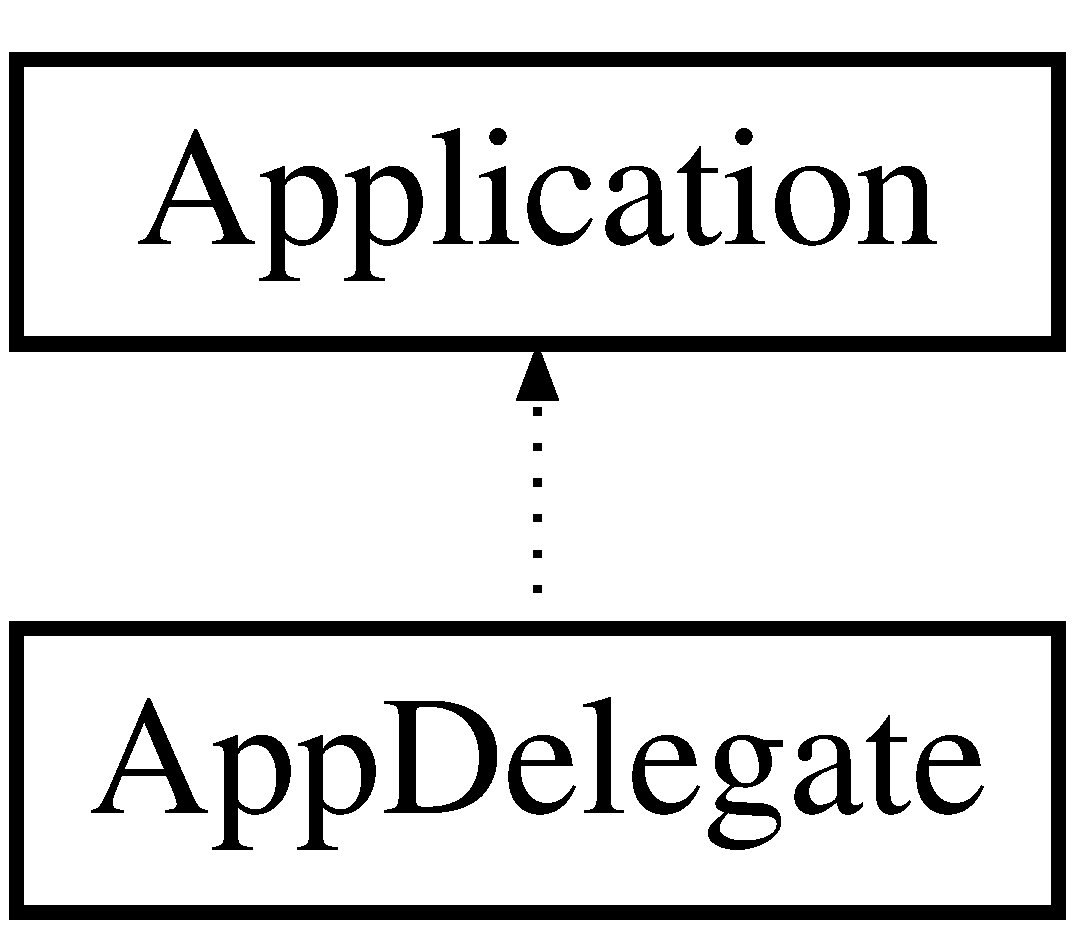
\includegraphics[height=2.000000cm]{class_app_delegate}
\end{center}
\end{figure}
\subsection*{Public Member Functions}
\begin{DoxyCompactItemize}
\item 
virtual void {\bfseries init\+G\+L\+Context\+Attrs} ()\hypertarget{class_app_delegate_a2de4e8ab7d04bde311684e1d4ceb2c0f}{}\label{class_app_delegate_a2de4e8ab7d04bde311684e1d4ceb2c0f}

\item 
virtual bool \hyperlink{class_app_delegate_a68cbaed49edf7581dc59a09d5062fff3}{application\+Did\+Finish\+Launching} ()
\begin{DoxyCompactList}\small\item\em Implement Director and Scene init code here. \end{DoxyCompactList}\item 
virtual void \hyperlink{class_app_delegate_a17cb09777419781698324e0415bffd3a}{application\+Did\+Enter\+Background} ()
\begin{DoxyCompactList}\small\item\em The function be called when the application enter background. \end{DoxyCompactList}\item 
virtual void \hyperlink{class_app_delegate_ac4d653e3f74a91efef5f2def58fe3108}{application\+Will\+Enter\+Foreground} ()
\begin{DoxyCompactList}\small\item\em The function be called when the application enter foreground. \end{DoxyCompactList}\end{DoxyCompactItemize}


\subsection{Detailed Description}
The cocos2d Application. 

The reason for implement as private inheritance is to hide some interface call by Director. 

\subsection{Member Function Documentation}
\index{App\+Delegate@{App\+Delegate}!application\+Did\+Enter\+Background@{application\+Did\+Enter\+Background}}
\index{application\+Did\+Enter\+Background@{application\+Did\+Enter\+Background}!App\+Delegate@{App\+Delegate}}
\subsubsection[{\texorpdfstring{application\+Did\+Enter\+Background()}{applicationDidEnterBackground()}}]{\setlength{\rightskip}{0pt plus 5cm}void App\+Delegate\+::application\+Did\+Enter\+Background (
\begin{DoxyParamCaption}
{}
\end{DoxyParamCaption}
)\hspace{0.3cm}{\ttfamily [virtual]}}\hypertarget{class_app_delegate_a17cb09777419781698324e0415bffd3a}{}\label{class_app_delegate_a17cb09777419781698324e0415bffd3a}


The function be called when the application enter background. 


\begin{DoxyParams}{Parameters}
{\em the} & pointer of the application \\
\hline
\end{DoxyParams}
\index{App\+Delegate@{App\+Delegate}!application\+Did\+Finish\+Launching@{application\+Did\+Finish\+Launching}}
\index{application\+Did\+Finish\+Launching@{application\+Did\+Finish\+Launching}!App\+Delegate@{App\+Delegate}}
\subsubsection[{\texorpdfstring{application\+Did\+Finish\+Launching()}{applicationDidFinishLaunching()}}]{\setlength{\rightskip}{0pt plus 5cm}bool App\+Delegate\+::application\+Did\+Finish\+Launching (
\begin{DoxyParamCaption}
{}
\end{DoxyParamCaption}
)\hspace{0.3cm}{\ttfamily [virtual]}}\hypertarget{class_app_delegate_a68cbaed49edf7581dc59a09d5062fff3}{}\label{class_app_delegate_a68cbaed49edf7581dc59a09d5062fff3}


Implement Director and Scene init code here. 

\begin{DoxyReturn}{Returns}
true Initialize success, app continue. 

false Initialize failed, app terminate. 
\end{DoxyReturn}
\index{App\+Delegate@{App\+Delegate}!application\+Will\+Enter\+Foreground@{application\+Will\+Enter\+Foreground}}
\index{application\+Will\+Enter\+Foreground@{application\+Will\+Enter\+Foreground}!App\+Delegate@{App\+Delegate}}
\subsubsection[{\texorpdfstring{application\+Will\+Enter\+Foreground()}{applicationWillEnterForeground()}}]{\setlength{\rightskip}{0pt plus 5cm}void App\+Delegate\+::application\+Will\+Enter\+Foreground (
\begin{DoxyParamCaption}
{}
\end{DoxyParamCaption}
)\hspace{0.3cm}{\ttfamily [virtual]}}\hypertarget{class_app_delegate_ac4d653e3f74a91efef5f2def58fe3108}{}\label{class_app_delegate_ac4d653e3f74a91efef5f2def58fe3108}


The function be called when the application enter foreground. 


\begin{DoxyParams}{Parameters}
{\em the} & pointer of the application \\
\hline
\end{DoxyParams}


The documentation for this class was generated from the following files\+:\begin{DoxyCompactItemize}
\item 
Classes/App\+Delegate.\+h\item 
Classes/App\+Delegate.\+cpp\end{DoxyCompactItemize}

\hypertarget{class_c_accessory_item}{}\section{C\+Accessory\+Item Class Reference}
\label{class_c_accessory_item}\index{C\+Accessory\+Item@{C\+Accessory\+Item}}
Inheritance diagram for C\+Accessory\+Item\+:\begin{figure}[H]
\begin{center}
\leavevmode
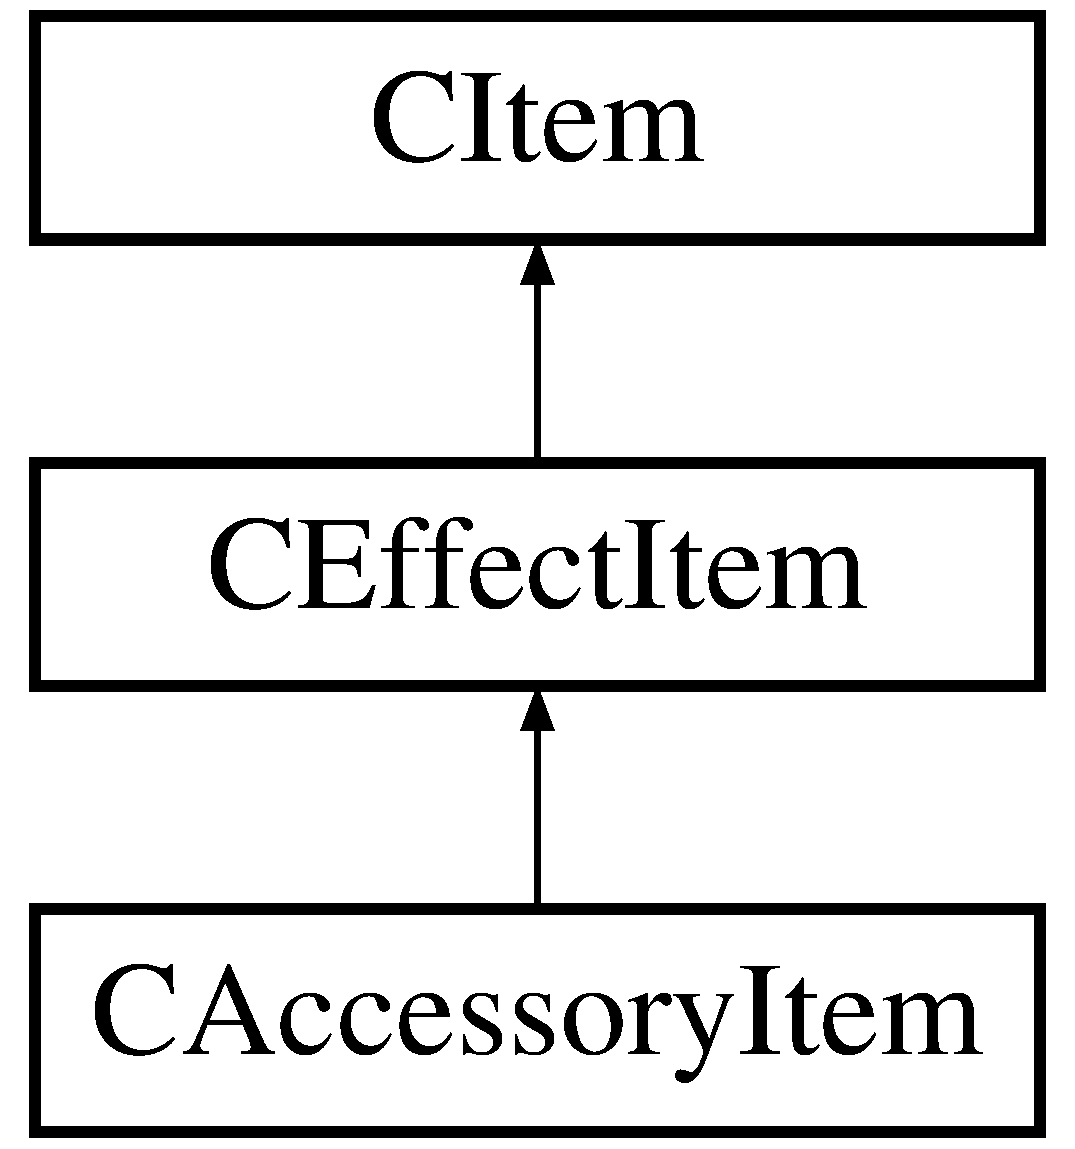
\includegraphics[height=3.000000cm]{class_c_accessory_item}
\end{center}
\end{figure}
\subsection*{Public Attributes}
\begin{DoxyCompactItemize}
\item 
std\+::vector$<$ std\+::pair$<$ std\+::string, int $>$ $>$ {\bfseries Material\+Set}\hypertarget{class_c_accessory_item_adc580086ec44d7bcc2b19512c79f19fe}{}\label{class_c_accessory_item_adc580086ec44d7bcc2b19512c79f19fe}

\end{DoxyCompactItemize}


The documentation for this class was generated from the following file\+:\begin{DoxyCompactItemize}
\item 
Classes/Item.\+h\end{DoxyCompactItemize}

\hypertarget{class_c_actor}{}\section{C\+Actor Class Reference}
\label{class_c_actor}\index{C\+Actor@{C\+Actor}}
Inheritance diagram for C\+Actor\+:\begin{figure}[H]
\begin{center}
\leavevmode
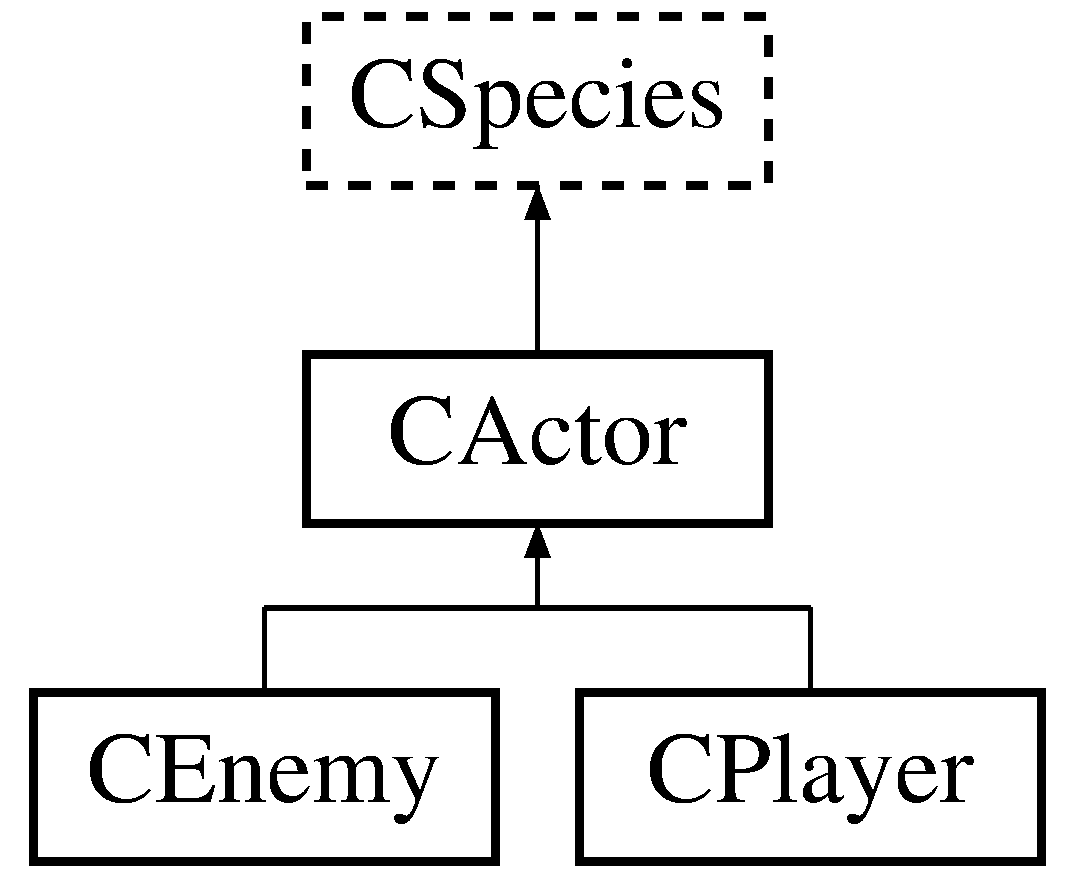
\includegraphics[height=3.000000cm]{class_c_actor}
\end{center}
\end{figure}
\subsection*{Public Member Functions}
\begin{DoxyCompactItemize}
\item 
{\bfseries C\+Actor} (const \hyperlink{class_c_species}{C\+Species} \&obj)\hypertarget{class_c_actor_a5bae9b0347cfe0c298ae14d1ddc4670a}{}\label{class_c_actor_a5bae9b0347cfe0c298ae14d1ddc4670a}

\item 
void {\bfseries First\+Set} (int \+\_\+playernum, int \+\_\+enemynum, int \+\_\+index, \hyperlink{class_c_text_box}{C\+Text\+Box} $\ast$$\ast$\+\_\+textbox, \hyperlink{class_c_cmd_list}{C\+Cmd\+List} $\ast$\+\_\+cmdlist, \hyperlink{class_c_log_window}{C\+Log\+Window} $\ast$\+\_\+log\+Window)\hypertarget{class_c_actor_aab10562dcc6b8601c3986d18b0636727}{}\label{class_c_actor_aab10562dcc6b8601c3986d18b0636727}

\item 
void {\bfseries Set\+Rect} (int \+\_\+cx, int \+\_\+cy)\hypertarget{class_c_actor_a7cffff5d6184ebe6bc1a39154a3f8503}{}\label{class_c_actor_a7cffff5d6184ebe6bc1a39154a3f8503}

\item 
bool {\bfseries Set\+System\+Img} (\hyperlink{class_c_b_img_bank}{C\+B\+Img\+Bank} $\ast$\+\_\+bimgbank)\hypertarget{class_c_actor_ab7adce3f7a83b3ccac0f961177ecf3da}{}\label{class_c_actor_ab7adce3f7a83b3ccac0f961177ecf3da}

\item 
bool {\bfseries Main} ()\hypertarget{class_c_actor_a988ae25f3fa7f8767415260b3ee00023}{}\label{class_c_actor_a988ae25f3fa7f8767415260b3ee00023}

\item 
bool {\bfseries Do} ()\hypertarget{class_c_actor_a1c9fd5d3fa2eb222ff4c4bf94bd58140}{}\label{class_c_actor_a1c9fd5d3fa2eb222ff4c4bf94bd58140}

\item 
virtual void {\bfseries Draw} (int \+\_\+dx=0, int \+\_\+dy=0)=0\hypertarget{class_c_actor_ac200b40b264c90ac18641ae70913924e}{}\label{class_c_actor_ac200b40b264c90ac18641ae70913924e}

\item 
int {\bfseries Get\+Actor\+Index} () const \hypertarget{class_c_actor_afe5b8dc29fe5f77fa972ca6d0c99c109}{}\label{class_c_actor_afe5b8dc29fe5f77fa972ca6d0c99c109}

\item 
int {\bfseries Get\+Index} () const \hypertarget{class_c_actor_aad14d3764562877bf0c479ff596edc6a}{}\label{class_c_actor_aad14d3764562877bf0c479ff596edc6a}

\item 
bool {\bfseries Is\+Player} () const \hypertarget{class_c_actor_aae1a50d017aa77b7a49eb78c2e8e3763}{}\label{class_c_actor_aae1a50d017aa77b7a49eb78c2e8e3763}

\item 
bool {\bfseries Get\+Alive} () const \hypertarget{class_c_actor_aa59b20d55ebf6052b24ebd62e8408f70}{}\label{class_c_actor_aa59b20d55ebf6052b24ebd62e8408f70}

\item 
int {\bfseries Get\+Visible\+Status} () const \hypertarget{class_c_actor_a5c12c729269aaebb111a511f70a37a1c}{}\label{class_c_actor_a5c12c729269aaebb111a511f70a37a1c}

\item 
bool {\bfseries Get\+Visible} () const \hypertarget{class_c_actor_a614c99a06241d60e3f4f76b69062bf43}{}\label{class_c_actor_a614c99a06241d60e3f4f76b69062bf43}

\item 
void {\bfseries Set\+Visible} (bool \+\_\+visible)\hypertarget{class_c_actor_a6b52a3a18435cc3c3c20940aadbb2b2e}{}\label{class_c_actor_a6b52a3a18435cc3c3c20940aadbb2b2e}

\item 
int {\bfseries Get\+Atk} () const \hypertarget{class_c_actor_a638d017fe2e6a9fe88b1e4f685ffedbd}{}\label{class_c_actor_a638d017fe2e6a9fe88b1e4f685ffedbd}

\item 
int {\bfseries Get\+Def} ()\hypertarget{class_c_actor_a583ce9ec2f0868fa4793a3441bc196d8}{}\label{class_c_actor_a583ce9ec2f0868fa4793a3441bc196d8}

\item 
int {\bfseries Get\+Hp} () const \hypertarget{class_c_actor_a99584b792244713fa540f45e9267f4c3}{}\label{class_c_actor_a99584b792244713fa540f45e9267f4c3}

\item 
int {\bfseries Get\+Max\+Hp} () const \hypertarget{class_c_actor_a33abdda7a572c5c58120fbf17e68ab74}{}\label{class_c_actor_a33abdda7a572c5c58120fbf17e68ab74}

\item 
\hyperlink{structtrick__tag}{trick\+\_\+tag} const $\ast$ {\bfseries Get\+Now\+Trick} () const \hypertarget{class_c_actor_aa286c738d69e5ae35686a6892e002789}{}\label{class_c_actor_aa286c738d69e5ae35686a6892e002789}

\item 
int {\bfseries Get\+Status} (int \+\_\+key)\hypertarget{class_c_actor_a2e6c26854a8be12e0af07fec2016183c}{}\label{class_c_actor_a2e6c26854a8be12e0af07fec2016183c}

\item 
void {\bfseries Set\+Status} (int \+\_\+key, int \+\_\+value)\hypertarget{class_c_actor_a7540692fbc4f3f3ecde0070566cb9ac8}{}\label{class_c_actor_a7540692fbc4f3f3ecde0070566cb9ac8}

\item 
int {\bfseries Damaged} (\hyperlink{class_c_actor}{C\+Actor} $\ast$\+\_\+attacker, \hyperlink{structtrick__tag}{trick\+\_\+tag} const $\ast$\+\_\+trick)\hypertarget{class_c_actor_affe0a553bc8b698bafbad9d4dc1b15cf}{}\label{class_c_actor_affe0a553bc8b698bafbad9d4dc1b15cf}

\item 
bool {\bfseries Check\+Bar\+Move} ()\hypertarget{class_c_actor_aacdd243e8678573bf6f1edca3b2abe09}{}\label{class_c_actor_aacdd243e8678573bf6f1edca3b2abe09}

\item 
void {\bfseries Set\+Target} (int \+\_\+target)\hypertarget{class_c_actor_a7ec02bed0a0f03d2648e48cb1197c1d2}{}\label{class_c_actor_a7ec02bed0a0f03d2648e48cb1197c1d2}

\item 
void {\bfseries Add\+Status\+Changer} (int \+\_\+kind, int \+\_\+power\+Percent, int \+\_\+time)\hypertarget{class_c_actor_a1d71b5ab2aad32d2caf6a651c5158339}{}\label{class_c_actor_a1d71b5ab2aad32d2caf6a651c5158339}

\item 
void {\bfseries Change\+Value} (int \+\_\+kind, int \+\_\+power\+Percent)\hypertarget{class_c_actor_a344f8eeb57ddf973bb95d647e0b742c9}{}\label{class_c_actor_a344f8eeb57ddf973bb95d647e0b742c9}

\item 
void {\bfseries Heal} (int \+\_\+percent)\hypertarget{class_c_actor_a85158d40366687dc3d2f4a11f42ddd90}{}\label{class_c_actor_a85158d40366687dc3d2f4a11f42ddd90}

\item 
\hyperlink{class_c_rect}{C\+Rect} {\bfseries Get\+Rect} () const \hypertarget{class_c_actor_ab74185243a96730c9992682bb4f1beb3}{}\label{class_c_actor_ab74185243a96730c9992682bb4f1beb3}

\end{DoxyCompactItemize}
\subsection*{Protected Types}
\begin{DoxyCompactItemize}
\item 
enum \{ {\bfseries V\+I\+S\+I\+B\+LE}, 
{\bfseries C\+H\+A\+N\+G\+I\+NG}, 
{\bfseries I\+N\+V\+I\+S\+I\+B\+LE}
 \}\hypertarget{class_c_actor_a72cc31c27f3d300119c0dae98d01eab7}{}\label{class_c_actor_a72cc31c27f3d300119c0dae98d01eab7}

\item 
enum {\bfseries mode\+\_\+tag} \{ \\*
{\bfseries P\+L\+AN}, 
{\bfseries P\+R\+E\+P\+A\+RE}, 
{\bfseries A\+C\+T\+I\+ON}, 
{\bfseries B\+E\+F\+O\+R\+E\+\_\+\+P\+L\+AN}, 
\\*
{\bfseries M\+O\+D\+E\+\_\+\+N\+UM}
 \}\hypertarget{class_c_actor_a6862dea3af171b967810ee5619738939}{}\label{class_c_actor_a6862dea3af171b967810ee5619738939}

\end{DoxyCompactItemize}
\subsection*{Protected Member Functions}
\begin{DoxyCompactItemize}
\item 
virtual void {\bfseries First\+Set2} ()\hypertarget{class_c_actor_aa7ccf97658107cd329f0dd669ce860ee}{}\label{class_c_actor_aa7ccf97658107cd329f0dd669ce860ee}

\item 
virtual void {\bfseries Set\+Extra\+Img} (\hyperlink{class_c_b_img_bank}{C\+B\+Img\+Bank} $\ast$\+\_\+b\+Img\+Bank)\hypertarget{class_c_actor_a113ab38eefb563c9bac95ed6766e7753}{}\label{class_c_actor_a113ab38eefb563c9bac95ed6766e7753}

\item 
void {\bfseries Draw\+\_\+\+Sub} (int \+\_\+dx=0, int \+\_\+dy=0)\hypertarget{class_c_actor_a0e23ae6d89e19d1f97c911c3a2979f83}{}\label{class_c_actor_a0e23ae6d89e19d1f97c911c3a2979f83}

\item 
virtual bool {\bfseries Plan} ()=0\hypertarget{class_c_actor_a5d3981af7c89ec304ee42edf0dc4d5e6}{}\label{class_c_actor_a5d3981af7c89ec304ee42edf0dc4d5e6}

\item 
virtual bool {\bfseries Action} ()=0\hypertarget{class_c_actor_a8488f83306f1bb4dde2144438f3b05c0}{}\label{class_c_actor_a8488f83306f1bb4dde2144438f3b05c0}

\end{DoxyCompactItemize}
\subsection*{Protected Attributes}
\begin{DoxyCompactItemize}
\item 
int {\bfseries P\+L\+A\+Y\+E\+R\+\_\+\+N\+UM}\hypertarget{class_c_actor_acaf5a0d56d6d559605c98d2e5d123dac}{}\label{class_c_actor_acaf5a0d56d6d559605c98d2e5d123dac}

\item 
int {\bfseries E\+N\+E\+M\+Y\+\_\+\+N\+UM}\hypertarget{class_c_actor_aad97041a2e44e401c6ab4a44584f8b95}{}\label{class_c_actor_aad97041a2e44e401c6ab4a44584f8b95}

\item 
int {\bfseries Actor\+Index}\hypertarget{class_c_actor_a170ca35b074b3f06b00eb414ce5d3692}{}\label{class_c_actor_a170ca35b074b3f06b00eb414ce5d3692}

\item 
int {\bfseries Index}\hypertarget{class_c_actor_adff20f8fc1557d60af909022ae07143f}{}\label{class_c_actor_adff20f8fc1557d60af909022ae07143f}

\item 
int {\bfseries Atk}\hypertarget{class_c_actor_a38772d20effe55a79298c1f8400b3e4e}{}\label{class_c_actor_a38772d20effe55a79298c1f8400b3e4e}

\item 
int {\bfseries Def}\hypertarget{class_c_actor_aeca99c74c0265ba588ef31bb7615de90}{}\label{class_c_actor_aeca99c74c0265ba588ef31bb7615de90}

\item 
double {\bfseries Spd}\hypertarget{class_c_actor_a086fb19095dfe955b05b00fefb0a9a6f}{}\label{class_c_actor_a086fb19095dfe955b05b00fefb0a9a6f}

\item 
int {\bfseries Max\+Hp}\hypertarget{class_c_actor_ab097e6436e9bc7c885f3a62f8177065f}{}\label{class_c_actor_ab097e6436e9bc7c885f3a62f8177065f}

\item 
bool {\bfseries Alive}\hypertarget{class_c_actor_ac3eca4b5efa2ecb6bedd4e5d30ab993b}{}\label{class_c_actor_ac3eca4b5efa2ecb6bedd4e5d30ab993b}

\item 
bool {\bfseries Visible}\hypertarget{class_c_actor_aa93d950eabf8b1f0b1693adfb7ff9770}{}\label{class_c_actor_aa93d950eabf8b1f0b1693adfb7ff9770}

\item 
enum C\+Actor\+:: \{ ... \}  {\bfseries Visible\+Status}\hypertarget{class_c_actor_a79714be7b20898795e0a2b16a1e78b38}{}\label{class_c_actor_a79714be7b20898795e0a2b16a1e78b38}

\item 
int {\bfseries Old\+Hp}\hypertarget{class_c_actor_a803b716cfe5e1a59911d527059e53d6e}{}\label{class_c_actor_a803b716cfe5e1a59911d527059e53d6e}

\item 
std\+::vector$<$ \hyperlink{structstatus_changer__tag}{status\+Changer\+\_\+tag} $>$ {\bfseries Status\+Changer\+List}\hypertarget{class_c_actor_a87bfed34f5f22e66cfc494a5d520133f}{}\label{class_c_actor_a87bfed34f5f22e66cfc494a5d520133f}

\item 
enum C\+Actor\+::mode\+\_\+tag {\bfseries Mode}\hypertarget{class_c_actor_ab2bfcc416a6879d7c69e980d77c7ebb8}{}\label{class_c_actor_ab2bfcc416a6879d7c69e980d77c7ebb8}

\item 
int {\bfseries Max\+Time\+Gauge}\hypertarget{class_c_actor_a86bc225671cd386221901b28d33804cc}{}\label{class_c_actor_a86bc225671cd386221901b28d33804cc}

\item 
\hyperlink{structtrick__tag}{trick\+\_\+tag} const $\ast$ {\bfseries Now\+Trick}\hypertarget{class_c_actor_ae398d65941b26ef5ae11f718c9117873}{}\label{class_c_actor_ae398d65941b26ef5ae11f718c9117873}

\item 
int {\bfseries Target}\hypertarget{class_c_actor_acf74fa1cd5a89bfb32599bb2d0927b84}{}\label{class_c_actor_acf74fa1cd5a89bfb32599bb2d0927b84}

\item 
\hyperlink{class_c_text_box}{C\+Text\+Box} $\ast$$\ast$ {\bfseries B\+\_\+\+Text\+Box\+\_\+pp}\hypertarget{class_c_actor_a7d30e5ece501e58905ca84190a6eca0c}{}\label{class_c_actor_a7d30e5ece501e58905ca84190a6eca0c}

\item 
\hyperlink{class_c_cmd_list}{C\+Cmd\+List} $\ast$ {\bfseries Cmd\+List}\hypertarget{class_c_actor_ad2178344644dfb6641d22270347a2642}{}\label{class_c_actor_ad2178344644dfb6641d22270347a2642}

\item 
\hyperlink{class_c_log_window}{C\+Log\+Window} $\ast$ {\bfseries Log\+Window}\hypertarget{class_c_actor_ac9d927740f7bd27888810f01b7adfbb8}{}\label{class_c_actor_ac9d927740f7bd27888810f01b7adfbb8}

\item 
\hyperlink{class_c_rect}{C\+Rect} {\bfseries Rect}\hypertarget{class_c_actor_a2966bbb88f033f4a22432e3337779665}{}\label{class_c_actor_a2966bbb88f033f4a22432e3337779665}

\item 
int {\bfseries Dx}\hypertarget{class_c_actor_ad92a8c0de5571aa8b22cd3feb9c481e3}{}\label{class_c_actor_ad92a8c0de5571aa8b22cd3feb9c481e3}

\item 
int {\bfseries Dy}\hypertarget{class_c_actor_ae3c51fdf009247a37a4ab868fa17a324}{}\label{class_c_actor_ae3c51fdf009247a37a4ab868fa17a324}

\end{DoxyCompactItemize}


The documentation for this class was generated from the following files\+:\begin{DoxyCompactItemize}
\item 
Classes/Actor.\+h\item 
Classes/Actor.\+cpp\end{DoxyCompactItemize}

\hypertarget{class_c_alchemist_manager}{}\section{C\+Alchemist\+Manager Class Reference}
\label{class_c_alchemist_manager}\index{C\+Alchemist\+Manager@{C\+Alchemist\+Manager}}
Inheritance diagram for C\+Alchemist\+Manager\+:\begin{figure}[H]
\begin{center}
\leavevmode
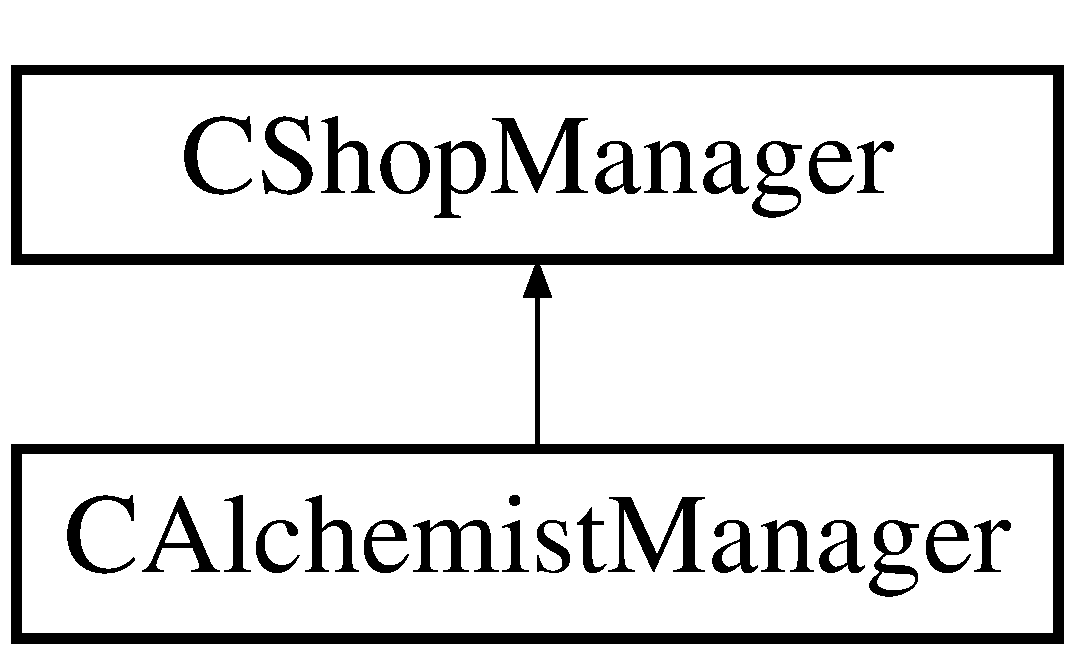
\includegraphics[height=2.000000cm]{class_c_alchemist_manager}
\end{center}
\end{figure}
\subsection*{Public Member Functions}
\begin{DoxyCompactItemize}
\item 
void {\bfseries Init} ()\hypertarget{class_c_alchemist_manager_ac16ed82c1b2b41f1053e3aa37107a07a}{}\label{class_c_alchemist_manager_ac16ed82c1b2b41f1053e3aa37107a07a}

\item 
bool {\bfseries Open\+Shop} (int \+\_\+index)\hypertarget{class_c_alchemist_manager_a2ba1d0c6e97d65e1834b9fafb8f6803c}{}\label{class_c_alchemist_manager_a2ba1d0c6e97d65e1834b9fafb8f6803c}

\end{DoxyCompactItemize}
\subsection*{Static Public Member Functions}
\begin{DoxyCompactItemize}
\item 
static \hyperlink{class_c_alchemist_manager}{C\+Alchemist\+Manager} $\ast$ {\bfseries Get\+Instance} ()\hypertarget{class_c_alchemist_manager_ac5317783685c1469cf8568658330a524}{}\label{class_c_alchemist_manager_ac5317783685c1469cf8568658330a524}

\end{DoxyCompactItemize}
\subsection*{Additional Inherited Members}


The documentation for this class was generated from the following files\+:\begin{DoxyCompactItemize}
\item 
Classes/Alchemist\+Manager.\+h\item 
Classes/Alchemist\+Manager.\+cpp\end{DoxyCompactItemize}

\hypertarget{class_c_alchemist_menu}{}\section{C\+Alchemist\+Menu Class Reference}
\label{class_c_alchemist_menu}\index{C\+Alchemist\+Menu@{C\+Alchemist\+Menu}}
Inheritance diagram for C\+Alchemist\+Menu\+:\begin{figure}[H]
\begin{center}
\leavevmode
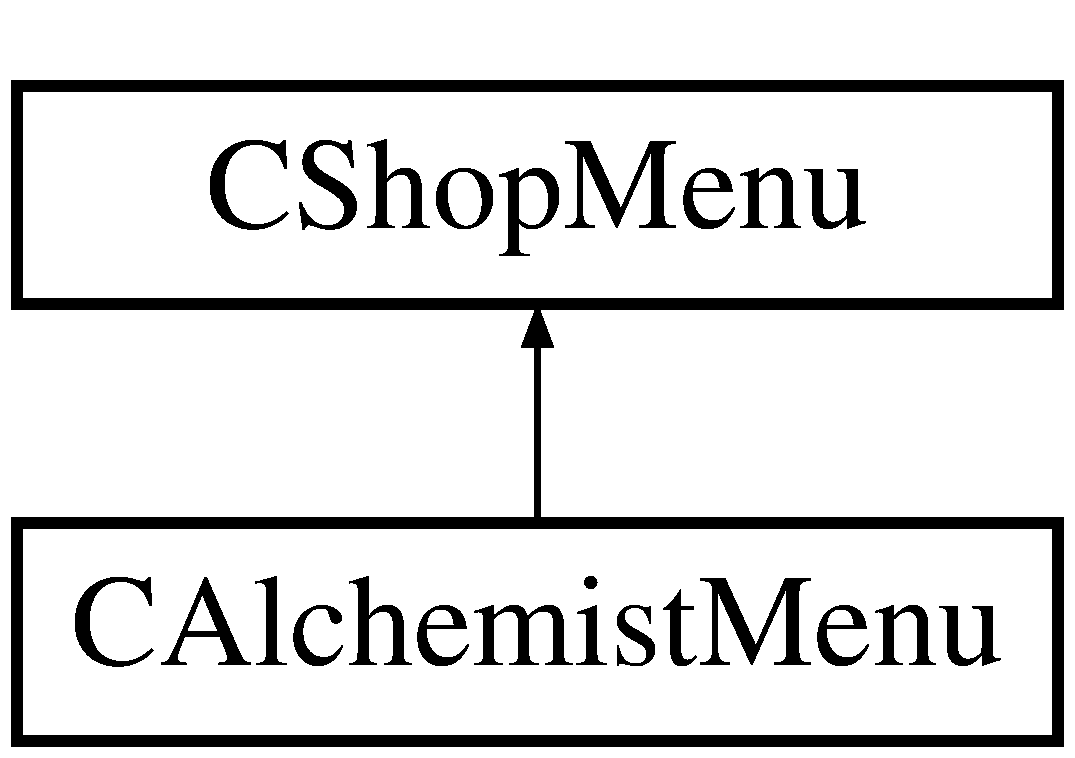
\includegraphics[height=2.000000cm]{class_c_alchemist_menu}
\end{center}
\end{figure}
\subsection*{Public Member Functions}
\begin{DoxyCompactItemize}
\item 
void {\bfseries Move} (int \+\_\+dir)\hypertarget{class_c_alchemist_menu_a93fdf7794b5ada5a88e9a78307419fa7}{}\label{class_c_alchemist_menu_a93fdf7794b5ada5a88e9a78307419fa7}

\item 
void {\bfseries Draw} ()\hypertarget{class_c_alchemist_menu_af7990a61a6007de3e3631a6ad868b7de}{}\label{class_c_alchemist_menu_af7990a61a6007de3e3631a6ad868b7de}

\item 
bool {\bfseries Buy} ()\hypertarget{class_c_alchemist_menu_a793f7b3eb8fa9d5e9bb1fad8e13bdf5f}{}\label{class_c_alchemist_menu_a793f7b3eb8fa9d5e9bb1fad8e13bdf5f}

\item 
bool {\bfseries Can\+Buy} ()\hypertarget{class_c_alchemist_menu_a1e7d49e982e9e557eeee946623dd902f}{}\label{class_c_alchemist_menu_a1e7d49e982e9e557eeee946623dd902f}

\item 
bool {\bfseries Can\+Close} ()\hypertarget{class_c_alchemist_menu_a47036666854ac5a10f91369e2bf8854f}{}\label{class_c_alchemist_menu_a47036666854ac5a10f91369e2bf8854f}

\end{DoxyCompactItemize}
\subsection*{Public Attributes}
\begin{DoxyCompactItemize}
\item 
std\+::vector$<$ std\+::vector$<$ std\+::pair$<$ std\+::string, int $>$ $>$ $>$ {\bfseries Current\+Material\+Set}\hypertarget{class_c_alchemist_menu_a92fb036a6e2961874aa7337b94f04d67}{}\label{class_c_alchemist_menu_a92fb036a6e2961874aa7337b94f04d67}

\end{DoxyCompactItemize}


The documentation for this class was generated from the following files\+:\begin{DoxyCompactItemize}
\item 
Classes/Alchemist\+Manager.\+h\item 
Classes/Alchemist\+Manager.\+cpp\end{DoxyCompactItemize}

\hypertarget{class_c_battle}{}\section{C\+Battle Class Reference}
\label{class_c_battle}\index{C\+Battle@{C\+Battle}}
Inheritance diagram for C\+Battle\+:\begin{figure}[H]
\begin{center}
\leavevmode
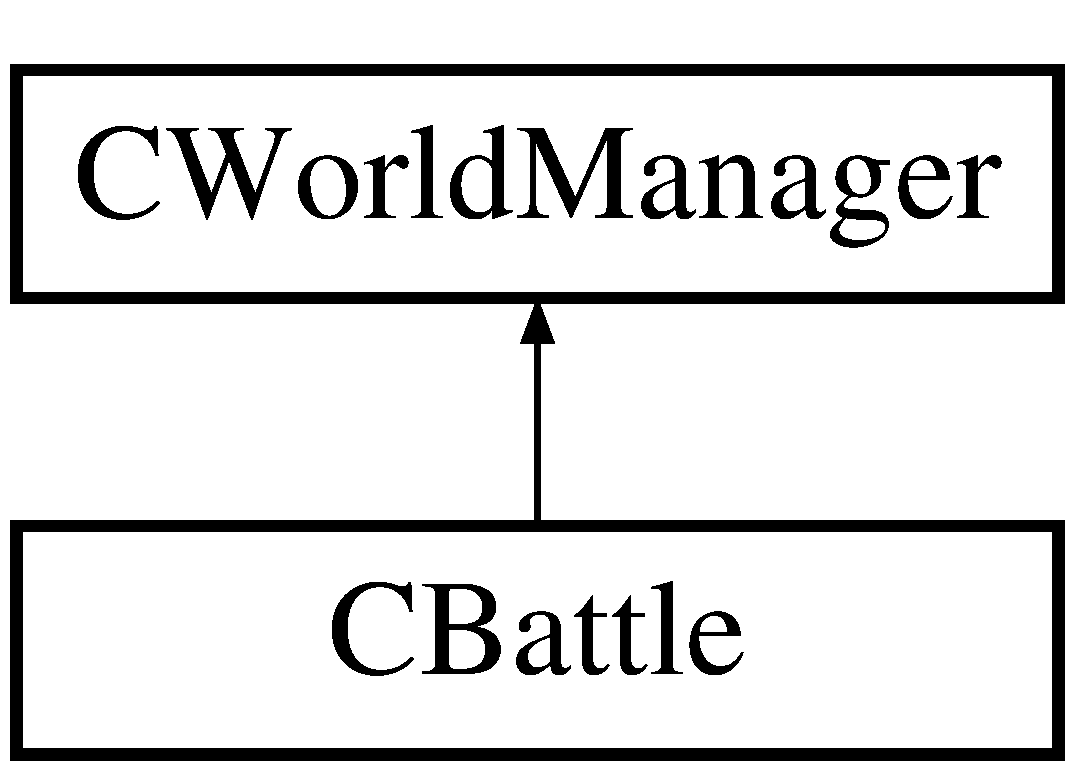
\includegraphics[height=2.000000cm]{class_c_battle}
\end{center}
\end{figure}
\subsection*{Classes}
\begin{DoxyCompactItemize}
\item 
class \hyperlink{class_c_battle_1_1_c_target_marker}{C\+Target\+Marker}
\end{DoxyCompactItemize}
\subsection*{Public Member Functions}
\begin{DoxyCompactItemize}
\item 
bool {\bfseries Init} ()\hypertarget{class_c_battle_ad4288e53bf58336701344736e71a65f9}{}\label{class_c_battle_ad4288e53bf58336701344736e71a65f9}

\item 
\hyperlink{class_c_menu_node}{C\+Menu\+Node} $\ast$ {\bfseries Get\+Field\+Status\+Menu\+Front\+Node} (const char \+\_\+parent\+Label\mbox{[}32\mbox{]})\hypertarget{class_c_battle_ad6799bcab4e9db10d5c4d81aab5c4ce5}{}\label{class_c_battle_ad6799bcab4e9db10d5c4d81aab5c4ce5}

\item 
void {\bfseries Update\+Field\+Player\+Accesssory\+Menu} (\hyperlink{class_c_menu_node}{C\+Menu\+Node} $\ast$\+\_\+player\+Node\+Parent)\hypertarget{class_c_battle_ad73a837f6724042dabec35d85ede91e4}{}\label{class_c_battle_ad73a837f6724042dabec35d85ede91e4}

\item 
void {\bfseries Update\+Player\+Accesssory\+Menu} (\hyperlink{class_c_menu_node}{C\+Menu\+Node} $\ast$\+\_\+player\+Node)\hypertarget{class_c_battle_ae51c1961332588459c81f9b8383c4357}{}\label{class_c_battle_ae51c1961332588459c81f9b8383c4357}

\item 
void {\bfseries Battle\+Ready} (\hyperlink{class_c_flag_set}{C\+Flag\+Set} $\ast$\+\_\+flagset\+\_\+p, \hyperlink{class_c_map}{C\+Map} $\ast$\+\_\+map\+\_\+p, \hyperlink{class_c_eve_manager}{C\+Eve\+Manager} $\ast$\+\_\+evemanager\+\_\+p)\hypertarget{class_c_battle_aa7c067df082cdf0790580bdba32e0363}{}\label{class_c_battle_aa7c067df082cdf0790580bdba32e0363}

\item 
void {\bfseries Battle\+Start} (int $\ast$\+\_\+result, \hyperlink{class_c_cmd_list}{C\+Cmd\+List} $\ast$\+\_\+fieldcmdlist\+\_\+p)\hypertarget{class_c_battle_ad264d63f91b14627d7a207e71478a404}{}\label{class_c_battle_ad264d63f91b14627d7a207e71478a404}

\item 
void {\bfseries Battle\+Setting} (const char $\ast$\+\_\+wincommand, const char $\ast$\+\_\+losecommand)\hypertarget{class_c_battle_a277f05cdd55dfbf28e21cbcdd7d4e325}{}\label{class_c_battle_a277f05cdd55dfbf28e21cbcdd7d4e325}

\item 
bool {\bfseries Check\+Encount} (int \+\_\+mapnum, int \+\_\+chipnum)\hypertarget{class_c_battle_a3af6b934068757e5eb62ef786360dd2c}{}\label{class_c_battle_a3af6b934068757e5eb62ef786360dd2c}

\item 
void \hyperlink{class_c_battle_ac416d83a1e6f4d2ff8c744023869c054}{Draw} (bool \+\_\+screenflip=false, bool \+\_\+textshowingstop=false, int dx=0, int dy=0, bool \+\_\+playeralsoshake=false)
\item 
void {\bfseries Change\+Text\+Mode} (bool \+\_\+box, const char $\ast$\+\_\+eventtext=N\+U\+LL)\hypertarget{class_c_battle_a6adcdc1aa707eb768aa311a784c98a98}{}\label{class_c_battle_a6adcdc1aa707eb768aa311a784c98a98}

\item 
int {\bfseries Get\+Actor\+Num} () const \hypertarget{class_c_battle_a34bde26f083675ba06d8793b1af01df2}{}\label{class_c_battle_a34bde26f083675ba06d8793b1af01df2}

\item 
void {\bfseries Set\+Back\+Ground} (const char $\ast$\+\_\+pickey)\hypertarget{class_c_battle_a6239d9c48096fe2487f0ff1c68d11062}{}\label{class_c_battle_a6239d9c48096fe2487f0ff1c68d11062}

\item 
void {\bfseries Set\+Back\+Ground} (int \+\_\+mapnum, int \+\_\+chipnum=-\/1)\hypertarget{class_c_battle_a8a885868777f55a0124e9463f83f8ea0}{}\label{class_c_battle_a8a885868777f55a0124e9463f83f8ea0}

\item 
void {\bfseries Set\+Player} ()\hypertarget{class_c_battle_a87d5e5b1da16875838881dcd04f04fa1}{}\label{class_c_battle_a87d5e5b1da16875838881dcd04f04fa1}

\item 
void {\bfseries Set\+Player} (const int \+\_\+player\+Num,...)\hypertarget{class_c_battle_a240dec65cd7817f3e012a27d62bd952d}{}\label{class_c_battle_a240dec65cd7817f3e012a27d62bd952d}

\item 
void {\bfseries Set\+Enemy} (const int \+\_\+enemy\+Num,...)\hypertarget{class_c_battle_ab566ace6e3e4e3a3d2312642d44e0459}{}\label{class_c_battle_ab566ace6e3e4e3a3d2312642d44e0459}

\item 
void {\bfseries Set\+Enemy} (std\+::vector$<$ std\+::string $>$ \+\_\+enemy\+List)\hypertarget{class_c_battle_a8275dbc7c3f8b8f12ab51ef97efd8960}{}\label{class_c_battle_a8275dbc7c3f8b8f12ab51ef97efd8960}

\item 
void {\bfseries Set\+Enemy} (std\+::vector$<$ \hyperlink{class_c_enemy_species}{C\+Enemy\+Species} $\ast$ $>$ \+\_\+enemy\+Party)\hypertarget{class_c_battle_a671882f3bbfe8b6a34a3a65160447894}{}\label{class_c_battle_a671882f3bbfe8b6a34a3a65160447894}

\item 
void {\bfseries Manage\+Attack} (int \+\_\+attacker\+Actor\+Index, int \+\_\+target\+Actor\+Index, \hyperlink{structtrick__tag}{trick\+\_\+tag} const $\ast$\+\_\+trick)\hypertarget{class_c_battle_a4c5aafcdc5093d314d73c78196082e39}{}\label{class_c_battle_a4c5aafcdc5093d314d73c78196082e39}

\item 
void {\bfseries Invoke\+Side\+Effect} (\hyperlink{structside_effect__tag}{side\+Effect\+\_\+tag} \+\_\+side\+Effect, int \+\_\+invoker\+Actor\+Index, int \+\_\+cursor\+Target\+Actor\+Index)\hypertarget{class_c_battle_a281ea23b83e29651bc5d8ffeee52f795}{}\label{class_c_battle_a281ea23b83e29651bc5d8ffeee52f795}

\item 
void {\bfseries Add\+Attention} (int \+\_\+enemy\+Index, int \+\_\+player\+Index, int \+\_\+value)\hypertarget{class_c_battle_a7960e2044172396ea8bf5674ebee61a8}{}\label{class_c_battle_a7960e2044172396ea8bf5674ebee61a8}

\item 
void {\bfseries Set\+Attention} (int \+\_\+enemy\+Index, int \+\_\+player\+Index, int \+\_\+value)\hypertarget{class_c_battle_adb7548ecf000b3ce3b0f8cd8c6b5db83}{}\label{class_c_battle_adb7548ecf000b3ce3b0f8cd8c6b5db83}

\end{DoxyCompactItemize}
\subsection*{Static Public Member Functions}
\begin{DoxyCompactItemize}
\item 
static \hyperlink{class_c_battle}{C\+Battle} $\ast$ {\bfseries Get\+Instance} ()\hypertarget{class_c_battle_a8e2e28c3ccfef842dc884e033b49fad6}{}\label{class_c_battle_a8e2e28c3ccfef842dc884e033b49fad6}

\end{DoxyCompactItemize}
\subsection*{Public Attributes}
\begin{DoxyCompactItemize}
\item 
class \hyperlink{class_c_battle_1_1_c_target_marker}{C\+Battle\+::\+C\+Target\+Marker} {\bfseries Target\+Marker}\hypertarget{class_c_battle_a834011fdbcaf9ce06c2a0aa09142daf7}{}\label{class_c_battle_a834011fdbcaf9ce06c2a0aa09142daf7}

\end{DoxyCompactItemize}
\subsection*{Additional Inherited Members}


\subsection{Member Function Documentation}
\index{C\+Battle@{C\+Battle}!Draw@{Draw}}
\index{Draw@{Draw}!C\+Battle@{C\+Battle}}
\subsubsection[{\texorpdfstring{Draw(bool \+\_\+screenflip=false, bool \+\_\+textshowingstop=false, int dx=0, int dy=0, bool \+\_\+playeralsoshake=false)}{Draw(bool _screenflip=false, bool _textshowingstop=false, int dx=0, int dy=0, bool _playeralsoshake=false)}}]{\setlength{\rightskip}{0pt plus 5cm}void C\+Battle\+::\+Draw (
\begin{DoxyParamCaption}
\item[{bool}]{\+\_\+screenflip = {\ttfamily false}, }
\item[{bool}]{\+\_\+textshowingstop = {\ttfamily false}, }
\item[{int}]{dx = {\ttfamily 0}, }
\item[{int}]{dy = {\ttfamily 0}, }
\item[{bool}]{\+\_\+playeralsoshake = {\ttfamily false}}
\end{DoxyParamCaption}
)\hspace{0.3cm}{\ttfamily [virtual]}}\hypertarget{class_c_battle_ac416d83a1e6f4d2ff8c744023869c054}{}\label{class_c_battle_ac416d83a1e6f4d2ff8c744023869c054}
テスト用////////////////////////////////////////////////////////////////////////// 

Implements \hyperlink{class_c_world_manager}{C\+World\+Manager}.



The documentation for this class was generated from the following files\+:\begin{DoxyCompactItemize}
\item 
Classes/Battle.\+h\item 
Classes/Battle.\+cpp\end{DoxyCompactItemize}

\hypertarget{class_c_battle_calculator}{}\section{C\+Battle\+Calculator Class Reference}
\label{class_c_battle_calculator}\index{C\+Battle\+Calculator@{C\+Battle\+Calculator}}
\subsection*{Public Types}
\begin{DoxyCompactItemize}
\item 
enum {\bfseries value\+\_\+tag} \{ \\*
{\bfseries M\+A\+X\+HP}, 
{\bfseries A\+TK}, 
{\bfseries D\+EF}, 
{\bfseries S\+PD}, 
\\*
{\bfseries B\+A\+S\+E\+\_\+\+T\+R\+I\+CK}
 \}\hypertarget{class_c_battle_calculator_a6b79d0c94bc9fa32455c55d3a77500f9}{}\label{class_c_battle_calculator_a6b79d0c94bc9fa32455c55d3a77500f9}

\end{DoxyCompactItemize}
\subsection*{Static Public Member Functions}
\begin{DoxyCompactItemize}
\item 
static int {\bfseries Calc\+Trick\+Power} (int \+\_\+level)\hypertarget{class_c_battle_calculator_a80fb5d1a3b5d6ef9ced10481ffc1c87b}{}\label{class_c_battle_calculator_a80fb5d1a3b5d6ef9ced10481ffc1c87b}

\item 
static int {\bfseries Calc\+Base\+Trick\+Power} (int \+\_\+level, int \+\_\+gene)\hypertarget{class_c_battle_calculator_a7e85a846ac58e950ce5df17bf36691c2}{}\label{class_c_battle_calculator_a7e85a846ac58e950ce5df17bf36691c2}

\item 
static double {\bfseries Calc\+Spd} (int \+\_\+level, int \+\_\+gene)\hypertarget{class_c_battle_calculator_a6e4dc10111d25e7b4c114d8d21c865cd}{}\label{class_c_battle_calculator_a6e4dc10111d25e7b4c114d8d21c865cd}

\item 
static int {\bfseries Calc\+Value} (value\+\_\+tag \+\_\+key, int \+\_\+level, int \+\_\+gene)\hypertarget{class_c_battle_calculator_a740a5e4e35e67858eac286c7c42a0e98}{}\label{class_c_battle_calculator_a740a5e4e35e67858eac286c7c42a0e98}

\item 
static int {\bfseries Calc\+Gold} (int \+\_\+lv, int \+\_\+goldgene)\hypertarget{class_c_battle_calculator_ac614df8377f4426788a92f18f29a60c6}{}\label{class_c_battle_calculator_ac614df8377f4426788a92f18f29a60c6}

\item 
static int {\bfseries Calc\+Exp} (int \+\_\+lv, int \+\_\+expgene)\hypertarget{class_c_battle_calculator_aeb13adffa99b8676938e03bf78b37676}{}\label{class_c_battle_calculator_aeb13adffa99b8676938e03bf78b37676}

\end{DoxyCompactItemize}


The documentation for this class was generated from the following files\+:\begin{DoxyCompactItemize}
\item 
Classes/Battle\+Calculator.\+h\item 
Classes/Battle\+Calculator.\+cpp\end{DoxyCompactItemize}

\hypertarget{class_c_battle_cmd_manager}{}\section{C\+Battle\+Cmd\+Manager Class Reference}
\label{class_c_battle_cmd_manager}\index{C\+Battle\+Cmd\+Manager@{C\+Battle\+Cmd\+Manager}}
Inheritance diagram for C\+Battle\+Cmd\+Manager\+:\begin{figure}[H]
\begin{center}
\leavevmode
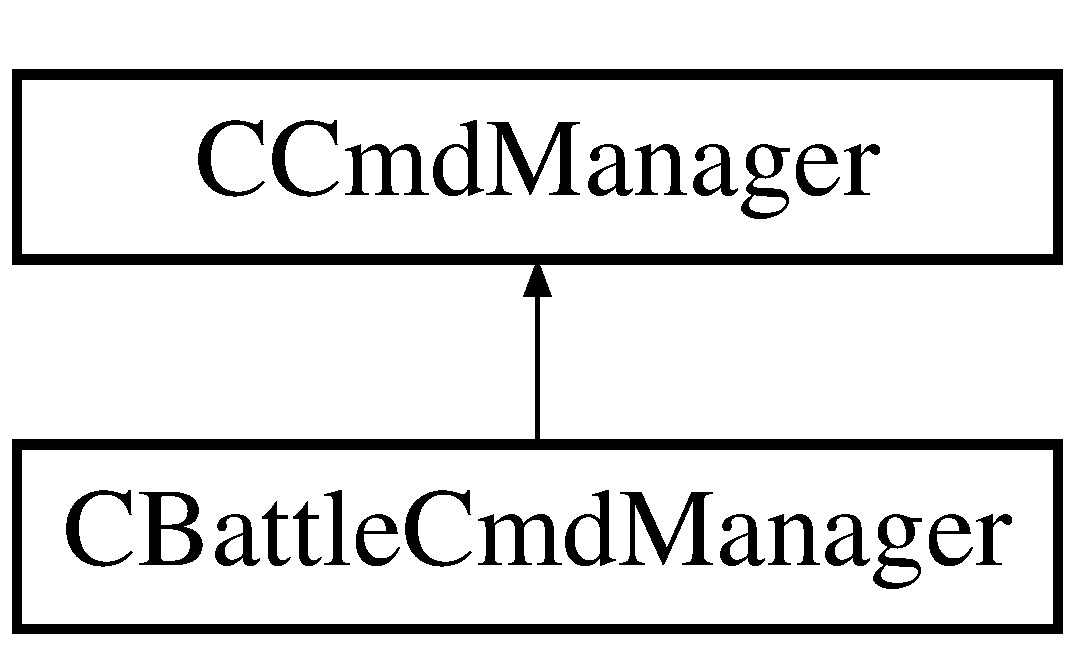
\includegraphics[height=2.000000cm]{class_c_battle_cmd_manager}
\end{center}
\end{figure}
\subsection*{Public Member Functions}
\begin{DoxyCompactItemize}
\item 
void {\bfseries Main} (\hyperlink{class_c_cmd_list}{C\+Cmd\+List} $\ast$\+\_\+cmdlist, \hyperlink{class_c_battle}{C\+Battle} $\ast$\+\_\+battle, \hyperlink{class_c_text_box}{C\+Text\+Box} $\ast$\+\_\+textbox)\hypertarget{class_c_battle_cmd_manager_a723ecfc71b6ab435f8573129ac067383}{}\label{class_c_battle_cmd_manager_a723ecfc71b6ab435f8573129ac067383}

\item 
void {\bfseries Init} (\hyperlink{class_c_map}{C\+Map} $\ast$\+\_\+map)\hypertarget{class_c_battle_cmd_manager_a564491ec7efb0db3f60cd826e2fecc62}{}\label{class_c_battle_cmd_manager_a564491ec7efb0db3f60cd826e2fecc62}

\end{DoxyCompactItemize}
\subsection*{Additional Inherited Members}


The documentation for this class was generated from the following files\+:\begin{DoxyCompactItemize}
\item 
Classes/Cmd\+Manager.\+h\item 
Classes/Cmd\+Manager.\+cpp\end{DoxyCompactItemize}

\hypertarget{class_c_battle_first_set_cmd_manager}{}\section{C\+Battle\+First\+Set\+Cmd\+Manager Class Reference}
\label{class_c_battle_first_set_cmd_manager}\index{C\+Battle\+First\+Set\+Cmd\+Manager@{C\+Battle\+First\+Set\+Cmd\+Manager}}
Inheritance diagram for C\+Battle\+First\+Set\+Cmd\+Manager\+:\begin{figure}[H]
\begin{center}
\leavevmode
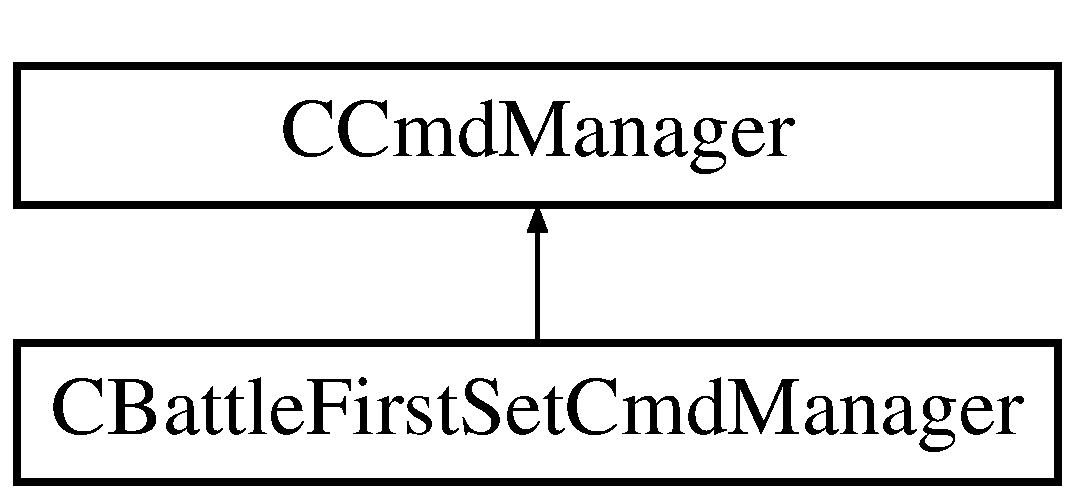
\includegraphics[height=2.000000cm]{class_c_battle_first_set_cmd_manager}
\end{center}
\end{figure}
\subsection*{Public Member Functions}
\begin{DoxyCompactItemize}
\item 
void {\bfseries Main} (\hyperlink{class_c_cmd_list}{C\+Cmd\+List} $\ast$\+\_\+cmdlist, \hyperlink{class_c_b_img_bank}{C\+B\+Img\+Bank} $\ast$\+\_\+bimgbank, \hyperlink{class_c_player_species_manager}{C\+Player\+Species\+Manager} $\ast$\+\_\+player\+Species\+Manager, \hyperlink{class_c_enemy_species_manager}{C\+Enemy\+Species\+Manager} $\ast$\+\_\+enemy\+Species\+Manager, \hyperlink{class_c_trick_manager}{C\+Trick\+Manager} $\ast$\+\_\+trick\+Manager)\hypertarget{class_c_battle_first_set_cmd_manager_a7b8dd4aed45613fb84f85a7729f6999b}{}\label{class_c_battle_first_set_cmd_manager_a7b8dd4aed45613fb84f85a7729f6999b}

\end{DoxyCompactItemize}
\subsection*{Additional Inherited Members}


The documentation for this class was generated from the following files\+:\begin{DoxyCompactItemize}
\item 
Classes/Cmd\+Manager.\+h\item 
Classes/Cmd\+Manager.\+cpp\end{DoxyCompactItemize}

\hypertarget{class_c_battle_log}{}\section{C\+Battle\+Log Class Reference}
\label{class_c_battle_log}\index{C\+Battle\+Log@{C\+Battle\+Log}}
Inheritance diagram for C\+Battle\+Log\+:\begin{figure}[H]
\begin{center}
\leavevmode
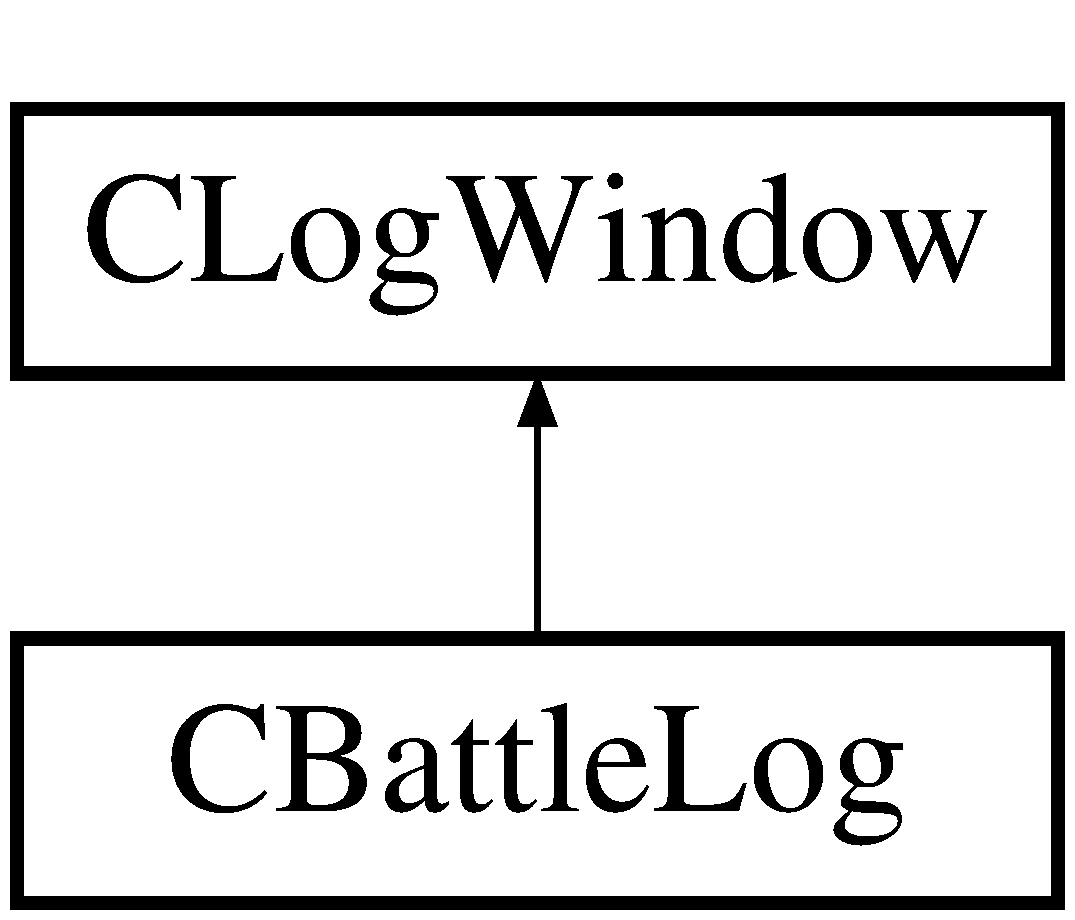
\includegraphics[height=2.000000cm]{class_c_battle_log}
\end{center}
\end{figure}
\subsection*{Public Member Functions}
\begin{DoxyCompactItemize}
\item 
void {\bfseries Init} (int \+\_\+smallposx, int \+\_\+posy, int \+\_\+smallwidth, int \+\_\+height, int \+\_\+box\+Color, int \+\_\+stock\+Line, int \+\_\+font\+Size, int \+\_\+font\+Color\+Main, int \+\_\+font\+Color\+Sub, \hyperlink{class_c_b_img_bank}{C\+B\+Img\+Bank} $\ast$\+\_\+b\+Img\+Bank)\hypertarget{class_c_battle_log_a200b786cd4c633935b6d44bd369a75d9}{}\label{class_c_battle_log_a200b786cd4c633935b6d44bd369a75d9}

\item 
void {\bfseries Draw} ()\hypertarget{class_c_battle_log_a37c7068cca23e16b613b11e3ae99f575}{}\label{class_c_battle_log_a37c7068cca23e16b613b11e3ae99f575}

\item 
void {\bfseries Clear} ()\hypertarget{class_c_battle_log_a9e99e2aa439e3d4d5f06d504a707dafb}{}\label{class_c_battle_log_a9e99e2aa439e3d4d5f06d504a707dafb}

\item 
bool {\bfseries Main} ()\hypertarget{class_c_battle_log_ae67a2f8aa2e999ea752fb8bb161dfa79}{}\label{class_c_battle_log_ae67a2f8aa2e999ea752fb8bb161dfa79}

\item 
void {\bfseries Set\+Window\+Mode} (bool \+\_\+full\+Mode)\hypertarget{class_c_battle_log_a001126def515556172030e22f0f6b8af}{}\label{class_c_battle_log_a001126def515556172030e22f0f6b8af}

\end{DoxyCompactItemize}
\subsection*{Additional Inherited Members}


The documentation for this class was generated from the following files\+:\begin{DoxyCompactItemize}
\item 
Classes/Log\+Window.\+h\item 
Classes/Log\+Window.\+cpp\end{DoxyCompactItemize}

\hypertarget{class_c_battle_menu}{}\section{C\+Battle\+Menu Class Reference}
\label{class_c_battle_menu}\index{C\+Battle\+Menu@{C\+Battle\+Menu}}
Inheritance diagram for C\+Battle\+Menu\+:\begin{figure}[H]
\begin{center}
\leavevmode
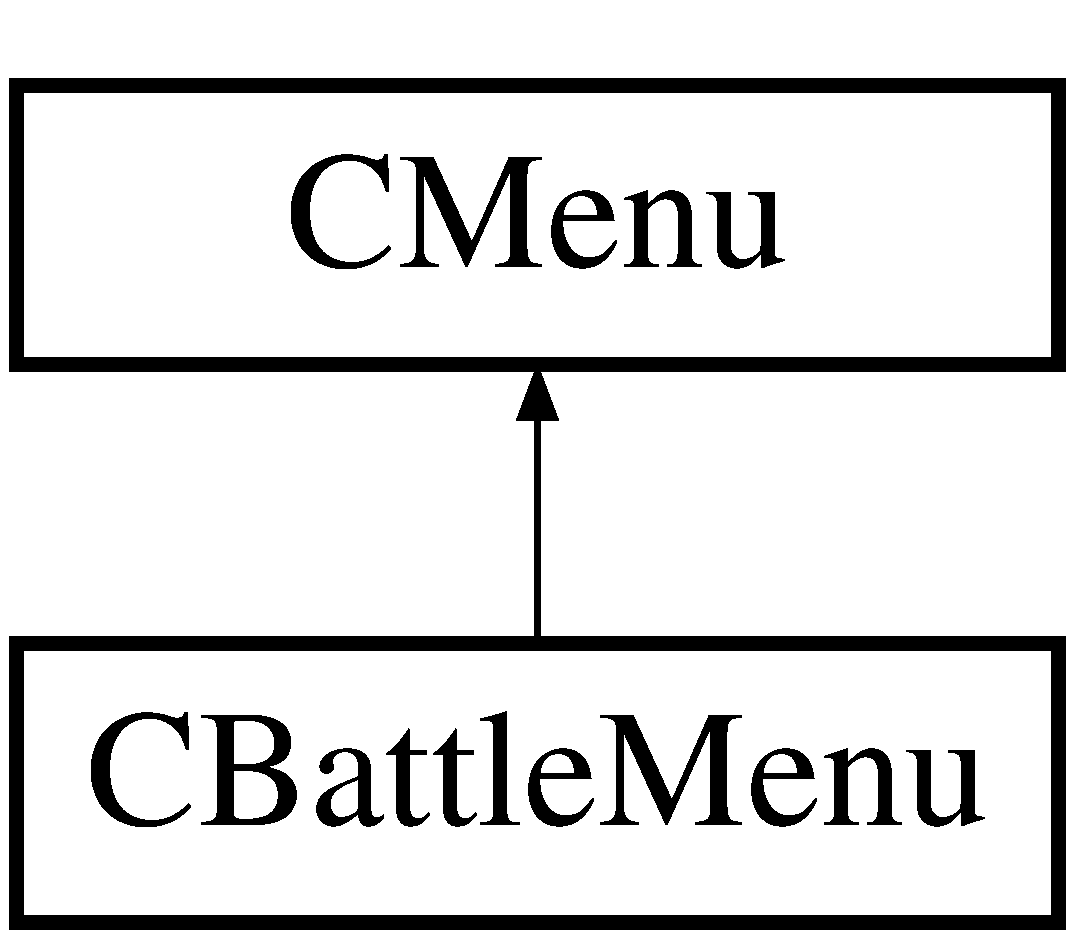
\includegraphics[height=2.000000cm]{class_c_battle_menu}
\end{center}
\end{figure}
\subsection*{Public Member Functions}
\begin{DoxyCompactItemize}
\item 
void {\bfseries Draw} ()\hypertarget{class_c_battle_menu_acf8df72fe00b1c74b08617cdd4d7a620}{}\label{class_c_battle_menu_acf8df72fe00b1c74b08617cdd4d7a620}

\end{DoxyCompactItemize}
\subsection*{Additional Inherited Members}


The documentation for this class was generated from the following files\+:\begin{DoxyCompactItemize}
\item 
Classes/Menu.\+h\item 
Classes/Menu.\+cpp\end{DoxyCompactItemize}

\hypertarget{class_c_b_img_bank}{}\section{C\+B\+Img\+Bank Class Reference}
\label{class_c_b_img_bank}\index{C\+B\+Img\+Bank@{C\+B\+Img\+Bank}}
Inheritance diagram for C\+B\+Img\+Bank\+:\begin{figure}[H]
\begin{center}
\leavevmode
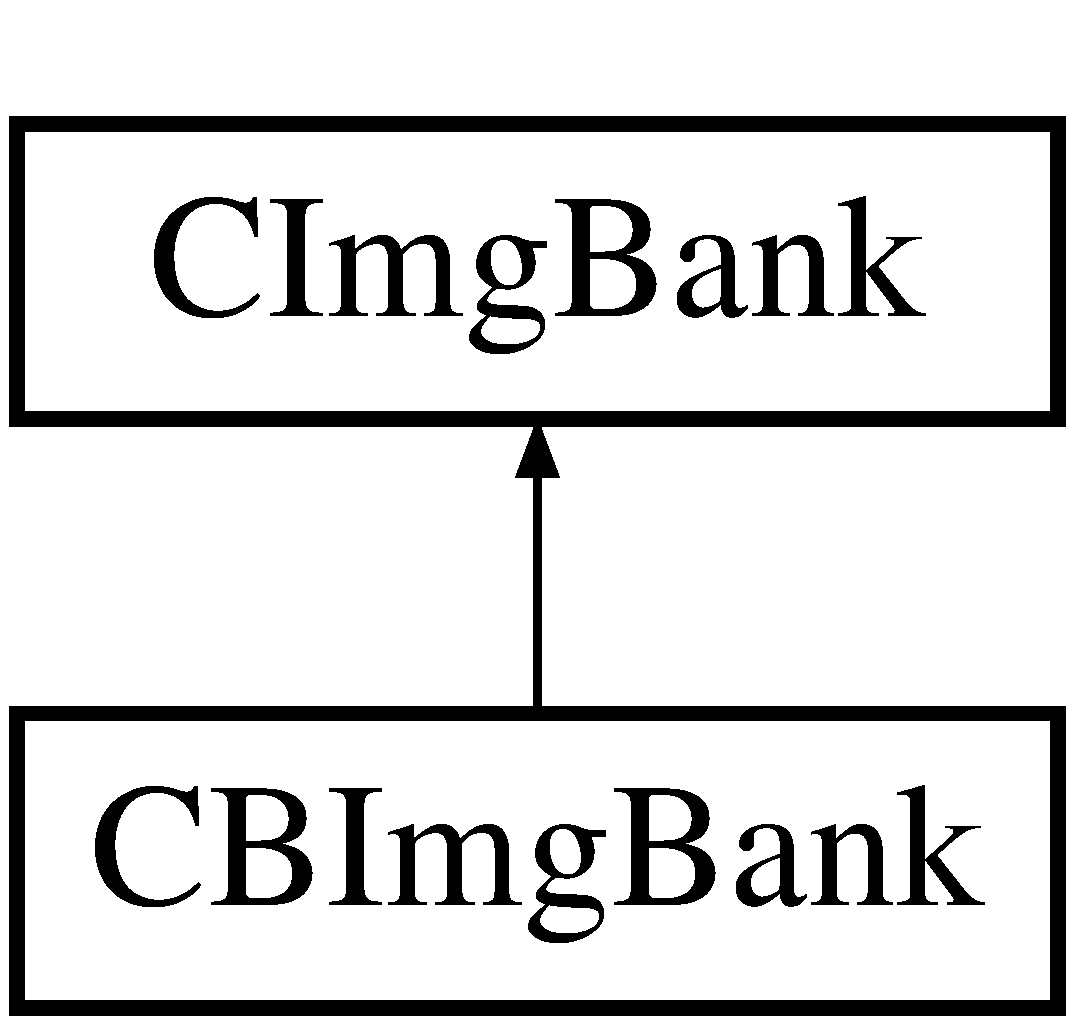
\includegraphics[height=2.000000cm]{class_c_b_img_bank}
\end{center}
\end{figure}
\subsection*{Public Member Functions}
\begin{DoxyCompactItemize}
\item 
void {\bfseries Clear} ()\hypertarget{class_c_b_img_bank_a9b6909dc6a06cba16e4ded1b78a9e707}{}\label{class_c_b_img_bank_a9b6909dc6a06cba16e4ded1b78a9e707}

\item 
void {\bfseries Init} ()\hypertarget{class_c_b_img_bank_ac01c6432a7e24ef726c829adc1c6c1b1}{}\label{class_c_b_img_bank_ac01c6432a7e24ef726c829adc1c6c1b1}

\item 
void {\bfseries Set\+Battle\+Back\+Ground} (const char $\ast$\+\_\+key, int \+\_\+mapnum, int \+\_\+chipnum=-\/1)\hypertarget{class_c_b_img_bank_a2efb5a1f7dec0e85b37afc470e63f039}{}\label{class_c_b_img_bank_a2efb5a1f7dec0e85b37afc470e63f039}

\item 
int {\bfseries Get\+Battle\+Back\+Ground} (int \+\_\+mapnum, int \+\_\+chipnum=-\/1)\hypertarget{class_c_b_img_bank_a44a9e2fdb0fa2bf79fae1ada748523b1}{}\label{class_c_b_img_bank_a44a9e2fdb0fa2bf79fae1ada748523b1}

\end{DoxyCompactItemize}


The documentation for this class was generated from the following files\+:\begin{DoxyCompactItemize}
\item 
Classes/B\+Img\+Bank.\+h\item 
Classes/B\+Img\+Bank.\+cpp\end{DoxyCompactItemize}

\hypertarget{class_c_cmd_list}{}\section{C\+Cmd\+List Class Reference}
\label{class_c_cmd_list}\index{C\+Cmd\+List@{C\+Cmd\+List}}
\subsection*{Public Member Functions}
\begin{DoxyCompactItemize}
\item 
void \hyperlink{class_c_cmd_list_a718e9fc133794256cc2815785a5ef20c}{Add} (const char $\ast$\+\_\+format,...)\hypertarget{class_c_cmd_list_a718e9fc133794256cc2815785a5ef20c}{}\label{class_c_cmd_list_a718e9fc133794256cc2815785a5ef20c}

\begin{DoxyCompactList}\small\item\em コマンドリスト/////////////////////////////////////////////////////////////////////// \end{DoxyCompactList}\item 
void {\bfseries Get} (char $\ast$\+\_\+cmd)\hypertarget{class_c_cmd_list_ae8125e1b77031faba6ad5dbf0dc465fc}{}\label{class_c_cmd_list_ae8125e1b77031faba6ad5dbf0dc465fc}

\item 
bool {\bfseries Empty} ()\hypertarget{class_c_cmd_list_a0d76c9c53f438f2df885c3f1d6e98ce0}{}\label{class_c_cmd_list_a0d76c9c53f438f2df885c3f1d6e98ce0}

\item 
void {\bfseries Clear} ()\hypertarget{class_c_cmd_list_ae2561b482fd1e96950398a4585291746}{}\label{class_c_cmd_list_ae2561b482fd1e96950398a4585291746}

\end{DoxyCompactItemize}


The documentation for this class was generated from the following files\+:\begin{DoxyCompactItemize}
\item 
Classes/Cmd\+List.\+h\item 
Classes/Cmd\+List.\+cpp\end{DoxyCompactItemize}

\hypertarget{class_c_cmd_manager}{}\section{C\+Cmd\+Manager Class Reference}
\label{class_c_cmd_manager}\index{C\+Cmd\+Manager@{C\+Cmd\+Manager}}
Inheritance diagram for C\+Cmd\+Manager\+:\begin{figure}[H]
\begin{center}
\leavevmode
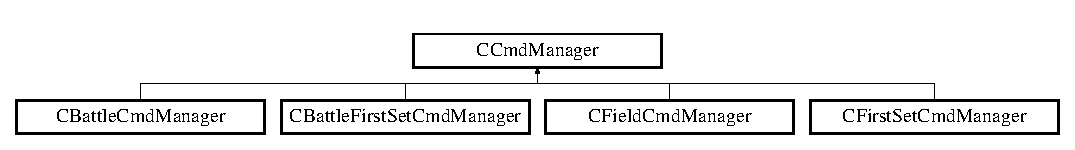
\includegraphics[height=1.564246cm]{class_c_cmd_manager}
\end{center}
\end{figure}
\subsection*{Protected Member Functions}
\begin{DoxyCompactItemize}
\item 
bool {\bfseries Next\+Command} (\hyperlink{class_c_cmd_list}{C\+Cmd\+List} $\ast$\+\_\+cmdlist, char $\ast$commandline, char $\ast$command, char $\ast$\&argument)\hypertarget{class_c_cmd_manager_a74d315e43349a013acd72fb0af98fb02}{}\label{class_c_cmd_manager_a74d315e43349a013acd72fb0af98fb02}

\item 
bool {\bfseries Arg\+Cut} (const char $\ast$\+\_\+command, char $\ast$\+\_\+argument, char $\ast$$\ast$\+\_\+arg, int \+\_\+argnum, bool \+\_\+warning=true, int \+\_\+minimum=0)\hypertarget{class_c_cmd_manager_ad0dc5d075df407798ff1646d523a078a}{}\label{class_c_cmd_manager_ad0dc5d075df407798ff1646d523a078a}

\item 
bool {\bfseries Field\+Cmd\+Solve} (const char $\ast$\+\_\+command, char $\ast$\+\_\+argument, \hyperlink{class_c_field}{C\+Field} $\ast$\+\_\+field, \hyperlink{class_c_map}{C\+Map} $\ast$\+\_\+map, \hyperlink{class_c_text_box}{C\+Text\+Box} $\ast$\+\_\+textbox, \hyperlink{class_c_eve_manager}{C\+Eve\+Manager} $\ast$\+\_\+evemanager)\hypertarget{class_c_cmd_manager_a5073fb7631fb3c8c51237726eb205593}{}\label{class_c_cmd_manager_a5073fb7631fb3c8c51237726eb205593}

\item 
bool {\bfseries System\+Cmd\+Solve} (const char $\ast$\+\_\+command, char $\ast$\+\_\+argument, \hyperlink{class_c_field}{C\+Field} $\ast$\+\_\+field, \hyperlink{class_c_map}{C\+Map} $\ast$\+\_\+map, \hyperlink{class_c_eve_manager}{C\+Eve\+Manager} $\ast$\+\_\+evemanager)\hypertarget{class_c_cmd_manager_a99d06c941837daf808274a5acfc807bd}{}\label{class_c_cmd_manager_a99d06c941837daf808274a5acfc807bd}

\item 
bool {\bfseries Window\+Cmd\+Solve} (const char $\ast$\+\_\+command, char $\ast$\+\_\+argument, \hyperlink{class_c_world_manager}{C\+World\+Manager} $\ast$\+\_\+worldmanager, \hyperlink{class_c_map}{C\+Map} $\ast$\+\_\+map, \hyperlink{class_c_text_box}{C\+Text\+Box} $\ast$\+\_\+textbox)\hypertarget{class_c_cmd_manager_a7adddb1eba418750408c24d2d6f70018}{}\label{class_c_cmd_manager_a7adddb1eba418750408c24d2d6f70018}

\item 
bool {\bfseries Text\+Cmd\+Solve} (const char $\ast$\+\_\+command, char $\ast$\+\_\+argument, \hyperlink{class_c_world_manager}{C\+World\+Manager} $\ast$\+\_\+worldmanager, \hyperlink{class_c_text_box}{C\+Text\+Box} $\ast$\+\_\+textbox)\hypertarget{class_c_cmd_manager_ae2c76d32ac406e7fd3e1858bd2cf9d21}{}\label{class_c_cmd_manager_ae2c76d32ac406e7fd3e1858bd2cf9d21}

\item 
bool {\bfseries Music\+System\+Cmd\+Solve} (const char $\ast$\+\_\+command, char $\ast$\+\_\+argument)\hypertarget{class_c_cmd_manager_ac2857c9400b5ef1a96867fa67e987a8c}{}\label{class_c_cmd_manager_ac2857c9400b5ef1a96867fa67e987a8c}

\item 
bool {\bfseries Music\+Cmd\+Solve} (const char $\ast$\+\_\+command, char $\ast$\+\_\+argument)\hypertarget{class_c_cmd_manager_af51d26aad1770e86fd475de812b99751}{}\label{class_c_cmd_manager_af51d26aad1770e86fd475de812b99751}

\item 
bool {\bfseries Battle\+System\+Cmd\+Solve} (const char $\ast$\+\_\+command, char $\ast$\+\_\+argument, \hyperlink{class_c_b_img_bank}{C\+B\+Img\+Bank} $\ast$\+\_\+bimgbank, \hyperlink{class_c_player_species_manager}{C\+Player\+Species\+Manager} $\ast$\+\_\+player\+Species\+Manager, \hyperlink{class_c_enemy_species_manager}{C\+Enemy\+Species\+Manager} $\ast$\+\_\+enemy\+Species\+Manager, \hyperlink{class_c_trick_manager}{C\+Trick\+Manager} $\ast$\+\_\+trick\+Manager)\hypertarget{class_c_cmd_manager_a99b57496818f386d50e79129e37f849a}{}\label{class_c_cmd_manager_a99b57496818f386d50e79129e37f849a}

\item 
bool {\bfseries Battle\+Cmd\+Solve} (const char $\ast$\+\_\+command, char $\ast$\+\_\+argument, \hyperlink{class_c_battle}{C\+Battle} $\ast$\+\_\+battle)\hypertarget{class_c_cmd_manager_a8c206d25a8c920ed68130da64f41efb5}{}\label{class_c_cmd_manager_a8c206d25a8c920ed68130da64f41efb5}

\end{DoxyCompactItemize}


The documentation for this class was generated from the following files\+:\begin{DoxyCompactItemize}
\item 
Classes/Cmd\+Manager.\+h\item 
Classes/Cmd\+Manager.\+cpp\end{DoxyCompactItemize}

\hypertarget{class_c_consumption_item}{}\section{C\+Consumption\+Item Class Reference}
\label{class_c_consumption_item}\index{C\+Consumption\+Item@{C\+Consumption\+Item}}
Inheritance diagram for C\+Consumption\+Item\+:\begin{figure}[H]
\begin{center}
\leavevmode
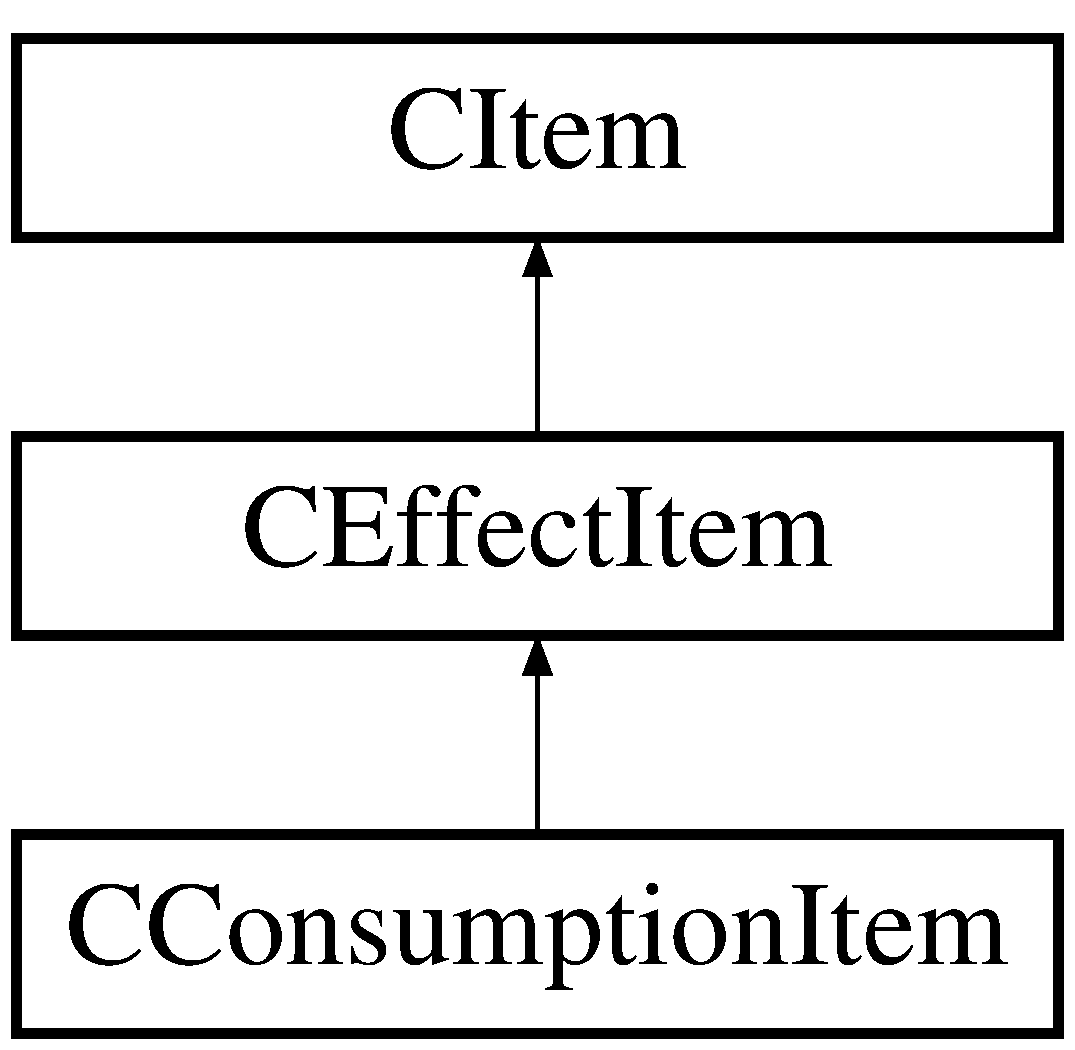
\includegraphics[height=3.000000cm]{class_c_consumption_item}
\end{center}
\end{figure}
\subsection*{Public Attributes}
\begin{DoxyCompactItemize}
\item 
bool {\bfseries Battle\+Usable}\hypertarget{class_c_consumption_item_a3e75872f2f45494c0582bf64f357e7ff}{}\label{class_c_consumption_item_a3e75872f2f45494c0582bf64f357e7ff}

\item 
int {\bfseries Wait\+Time}\hypertarget{class_c_consumption_item_a4904c0d42191c521ae0821d552da42c4}{}\label{class_c_consumption_item_a4904c0d42191c521ae0821d552da42c4}

\item 
target\+\_\+tag\+::type {\bfseries Target}\hypertarget{class_c_consumption_item_a9beb52aff1f3465a12218c9b965b3568}{}\label{class_c_consumption_item_a9beb52aff1f3465a12218c9b965b3568}

\end{DoxyCompactItemize}


The documentation for this class was generated from the following file\+:\begin{DoxyCompactItemize}
\item 
Classes/Item.\+h\end{DoxyCompactItemize}

\hypertarget{class_c_effect_item}{}\section{C\+Effect\+Item Class Reference}
\label{class_c_effect_item}\index{C\+Effect\+Item@{C\+Effect\+Item}}
Inheritance diagram for C\+Effect\+Item\+:\begin{figure}[H]
\begin{center}
\leavevmode
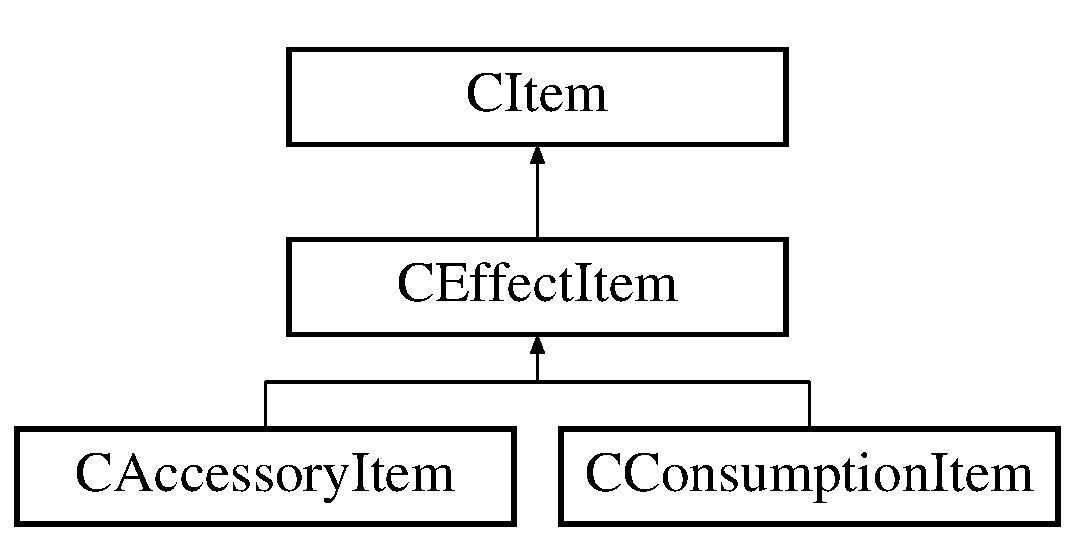
\includegraphics[height=3.000000cm]{class_c_effect_item}
\end{center}
\end{figure}
\subsection*{Public Attributes}
\begin{DoxyCompactItemize}
\item 
std\+::vector$<$ \hyperlink{structside_effect__tag}{side\+Effect\+\_\+tag} $>$ {\bfseries Side\+Effect\+Set}\hypertarget{class_c_effect_item_a3adaa85fe5314200248c98347d5dcd6f}{}\label{class_c_effect_item_a3adaa85fe5314200248c98347d5dcd6f}

\end{DoxyCompactItemize}


The documentation for this class was generated from the following file\+:\begin{DoxyCompactItemize}
\item 
Classes/Item.\+h\end{DoxyCompactItemize}

\hypertarget{class_c_enemy}{}\section{C\+Enemy Class Reference}
\label{class_c_enemy}\index{C\+Enemy@{C\+Enemy}}
Inheritance diagram for C\+Enemy\+:\begin{figure}[H]
\begin{center}
\leavevmode
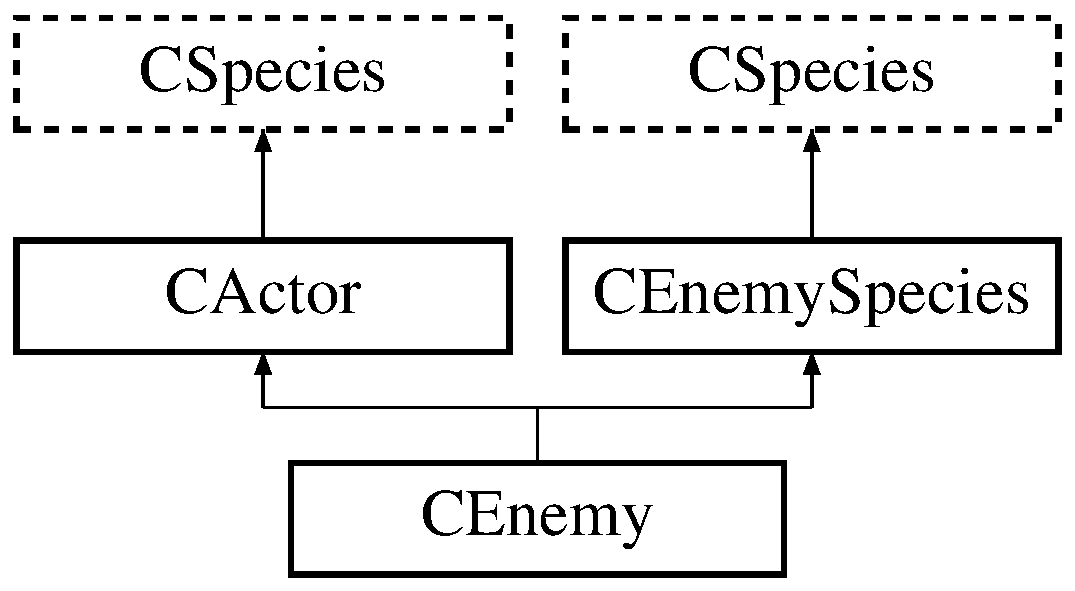
\includegraphics[height=3.000000cm]{class_c_enemy}
\end{center}
\end{figure}
\subsection*{Public Member Functions}
\begin{DoxyCompactItemize}
\item 
{\bfseries C\+Enemy} (const \hyperlink{class_c_enemy_species}{C\+Enemy\+Species} \&obj)\hypertarget{class_c_enemy_ab5c28f8725327379dfe64dfebc68d2bf}{}\label{class_c_enemy_ab5c28f8725327379dfe64dfebc68d2bf}

\item 
void {\bfseries Draw} (int \+\_\+dx=0, int \+\_\+dy=0)\hypertarget{class_c_enemy_aedd3ed5bad987073bc186a773ffd2c28}{}\label{class_c_enemy_aedd3ed5bad987073bc186a773ffd2c28}

\item 
void {\bfseries Battle\+Ready} (const \hyperlink{class_c_actor}{C\+Actor} $\ast$const $\ast$\+\_\+actor\+List, const int \+\_\+player\+Num, const int \+\_\+enemy\+Num)\hypertarget{class_c_enemy_a5e5f02fa87856b02da52805683fe2678}{}\label{class_c_enemy_a5e5f02fa87856b02da52805683fe2678}

\item 
void {\bfseries Add\+Attention} (int \+\_\+player\+Index, int \+\_\+value, \hyperlink{class_c_log_window}{C\+Log\+Window} $\ast$\+\_\+log\+Window=N\+U\+LL)\hypertarget{class_c_enemy_a34e14d379c133bec19a6f7ec31647a6b}{}\label{class_c_enemy_a34e14d379c133bec19a6f7ec31647a6b}

\item 
void {\bfseries Set\+Attention} (int \+\_\+player\+Index, int \+\_\+value)\hypertarget{class_c_enemy_a0ae40dfe0d249f6644fcaf3bfd89160c}{}\label{class_c_enemy_a0ae40dfe0d249f6644fcaf3bfd89160c}

\item 
std\+::vector$<$ std\+::string $>$ {\bfseries Get\+Drop\+Item\+List} ()\hypertarget{class_c_enemy_afe06e412b937daf27fcc21ee2d68a4f2}{}\label{class_c_enemy_afe06e412b937daf27fcc21ee2d68a4f2}

\end{DoxyCompactItemize}
\subsection*{Additional Inherited Members}


The documentation for this class was generated from the following files\+:\begin{DoxyCompactItemize}
\item 
Classes/Enemy.\+h\item 
Classes/Enemy.\+cpp\end{DoxyCompactItemize}

\hypertarget{class_c_enemy_a_i}{}\section{C\+Enemy\+AI Class Reference}
\label{class_c_enemy_a_i}\index{C\+Enemy\+AI@{C\+Enemy\+AI}}
\subsection*{Public Member Functions}
\begin{DoxyCompactItemize}
\item 
void {\bfseries Battle\+Ready} (const \hyperlink{class_c_actor}{C\+Actor} $\ast$const $\ast$\+\_\+actor\+List, const int \+\_\+player\+Num, const int \+\_\+enemy\+Num)\hypertarget{class_c_enemy_a_i_a686edd0c9def3e9e3d15db2875bc5e38}{}\label{class_c_enemy_a_i_a686edd0c9def3e9e3d15db2875bc5e38}

\item 
\hyperlink{class_c_enemy_planner}{C\+Enemy\+Planner} $\ast$ {\bfseries Set\+Planner} (\hyperlink{class_c_enemy_planner}{C\+Enemy\+Planner} $\ast$\+\_\+planner)\hypertarget{class_c_enemy_a_i_a1937e173f5e4de133e22a0b17bac3dd2}{}\label{class_c_enemy_a_i_a1937e173f5e4de133e22a0b17bac3dd2}

\item 
\hyperlink{class_c_enemy_targetter}{C\+Enemy\+Targetter} $\ast$ {\bfseries Set\+Targetter} (\hyperlink{class_c_enemy_targetter}{C\+Enemy\+Targetter} $\ast$\+\_\+targetter)\hypertarget{class_c_enemy_a_i_a7c0d802bc98c57d8fea078b7b7dd99f6}{}\label{class_c_enemy_a_i_a7c0d802bc98c57d8fea078b7b7dd99f6}

\item 
int {\bfseries Get\+Plan} (const \hyperlink{class_c_enemy}{C\+Enemy} $\ast$\+\_\+enemy)\hypertarget{class_c_enemy_a_i_a90f7d5697813517710f20412d1ca0634}{}\label{class_c_enemy_a_i_a90f7d5697813517710f20412d1ca0634}

\item 
int {\bfseries Get\+Target} (const \hyperlink{class_c_enemy}{C\+Enemy} $\ast$\+\_\+enemy)\hypertarget{class_c_enemy_a_i_a54bada58d6cf91bbfb54deaf86c4218b}{}\label{class_c_enemy_a_i_a54bada58d6cf91bbfb54deaf86c4218b}

\item 
bool {\bfseries Add\+Random\+Plan\+Set} (const unsigned int \+\_\+index, std\+::vector$<$ std\+::pair$<$ int, int $>$ $>$ \+\_\+plan\+List, bool \+\_\+clear=false)\hypertarget{class_c_enemy_a_i_ad538577e56076a3d43bdee2235e5083a}{}\label{class_c_enemy_a_i_ad538577e56076a3d43bdee2235e5083a}

\item 
void {\bfseries Add\+Attention} (int \+\_\+player\+Index, int \+\_\+value, \hyperlink{class_c_log_window}{C\+Log\+Window} $\ast$\+\_\+log\+Window=N\+U\+LL)\hypertarget{class_c_enemy_a_i_af5f75832f00bbc28af976893d15a6180}{}\label{class_c_enemy_a_i_af5f75832f00bbc28af976893d15a6180}

\item 
void {\bfseries Set\+Attention} (int \+\_\+player\+Index, int \+\_\+value)\hypertarget{class_c_enemy_a_i_ad3e318eec9e34d215a8b336a89ec75e0}{}\label{class_c_enemy_a_i_ad3e318eec9e34d215a8b336a89ec75e0}

\item 
void {\bfseries Draw} (const \hyperlink{class_c_enemy}{C\+Enemy} $\ast$\+\_\+enemy)\hypertarget{class_c_enemy_a_i_a6c8c0253c5ecb663bc1e73b868b4a5af}{}\label{class_c_enemy_a_i_a6c8c0253c5ecb663bc1e73b868b4a5af}

\end{DoxyCompactItemize}
\subsection*{Static Public Member Functions}
\begin{DoxyCompactItemize}
\item 
static void {\bfseries Set\+Attention\+Img} (int $\ast$\+\_\+marker\+Img, int \+\_\+board\+Img, int \+\_\+effect\+Img)\hypertarget{class_c_enemy_a_i_af0279ae7e871a9139c03517373c53b25}{}\label{class_c_enemy_a_i_af0279ae7e871a9139c03517373c53b25}

\end{DoxyCompactItemize}


The documentation for this class was generated from the following files\+:\begin{DoxyCompactItemize}
\item 
Classes/Enemy\+A\+I.\+h\item 
Classes/Enemy\+A\+I.\+cpp\end{DoxyCompactItemize}

\hypertarget{class_c_enemy_planner}{}\section{C\+Enemy\+Planner Class Reference}
\label{class_c_enemy_planner}\index{C\+Enemy\+Planner@{C\+Enemy\+Planner}}
Inheritance diagram for C\+Enemy\+Planner\+:\begin{figure}[H]
\begin{center}
\leavevmode
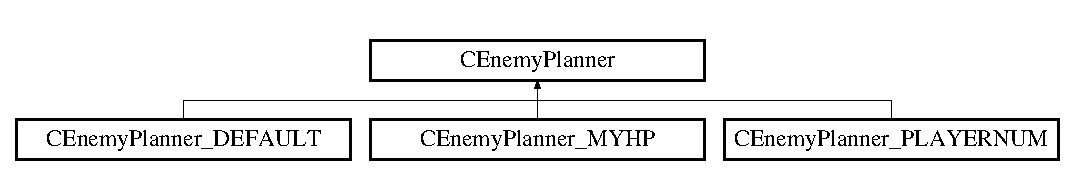
\includegraphics[height=1.914530cm]{class_c_enemy_planner}
\end{center}
\end{figure}
\subsection*{Public Member Functions}
\begin{DoxyCompactItemize}
\item 
{\bfseries C\+Enemy\+Planner} (std\+::string \+\_\+enemyname)\hypertarget{class_c_enemy_planner_aa37dda7cb289c53cfabd45b5992c57fa}{}\label{class_c_enemy_planner_aa37dda7cb289c53cfabd45b5992c57fa}

\item 
void {\bfseries Battle\+Ready} (const \hyperlink{class_c_actor}{C\+Actor} $\ast$const $\ast$\+\_\+actor\+List, const int \+\_\+player\+Num, const int \+\_\+enemy\+Num)\hypertarget{class_c_enemy_planner_a52c6974a32442debbaedebf14a45458b}{}\label{class_c_enemy_planner_a52c6974a32442debbaedebf14a45458b}

\item 
void {\bfseries Set\+Random\+Plan\+Set} (std\+::map$<$ int, std\+::vector$<$ std\+::pair$<$ int, int $>$ $>$ $>$ $\ast$\+\_\+random\+\_\+plan\+\_\+set)\hypertarget{class_c_enemy_planner_af89bcad6c1491139c2c3faf81f84f38a}{}\label{class_c_enemy_planner_af89bcad6c1491139c2c3faf81f84f38a}

\item 
std\+::string {\bfseries Get\+Name} () const \hypertarget{class_c_enemy_planner_a42d9f3358032f6cb1cd9804776cfc26e}{}\label{class_c_enemy_planner_a42d9f3358032f6cb1cd9804776cfc26e}

\item 
virtual int {\bfseries Get\+Plan} (const \hyperlink{class_c_enemy}{C\+Enemy} $\ast$\+\_\+enemy)=0\hypertarget{class_c_enemy_planner_ab49948ff6784b7b21d9a828f560daa40}{}\label{class_c_enemy_planner_ab49948ff6784b7b21d9a828f560daa40}

\end{DoxyCompactItemize}
\subsection*{Protected Member Functions}
\begin{DoxyCompactItemize}
\item 
int {\bfseries Calc\+Random\+Plan} (int \+\_\+random\+Plan\+\_\+key, const \hyperlink{class_c_enemy}{C\+Enemy} $\ast$\+\_\+enemy)\hypertarget{class_c_enemy_planner_a830dba5323b19e2534a361949bc785c3}{}\label{class_c_enemy_planner_a830dba5323b19e2534a361949bc785c3}

\end{DoxyCompactItemize}
\subsection*{Protected Attributes}
\begin{DoxyCompactItemize}
\item 
std\+::map$<$ int, std\+::vector$<$ std\+::pair$<$ int, int $>$ $>$ $>$ $\ast$ {\bfseries Random\+Plan\+Set}\hypertarget{class_c_enemy_planner_aa67925ceabbf73a42ca9b6d5d672b8bb}{}\label{class_c_enemy_planner_aa67925ceabbf73a42ca9b6d5d672b8bb}

\item 
const \hyperlink{class_c_actor}{C\+Actor} $\ast$const $\ast$ {\bfseries Actor}\hypertarget{class_c_enemy_planner_a8b8263d1eff7c1e301cf89a432acf169}{}\label{class_c_enemy_planner_a8b8263d1eff7c1e301cf89a432acf169}

\item 
int {\bfseries P\+L\+A\+Y\+E\+R\+\_\+\+N\+UM}\hypertarget{class_c_enemy_planner_a9bb42588ddd87d3773a2c206b62e80f3}{}\label{class_c_enemy_planner_a9bb42588ddd87d3773a2c206b62e80f3}

\item 
int {\bfseries E\+N\+E\+M\+Y\+\_\+\+N\+UM}\hypertarget{class_c_enemy_planner_a14c4bb52945b2755fb2230578ef761cd}{}\label{class_c_enemy_planner_a14c4bb52945b2755fb2230578ef761cd}

\end{DoxyCompactItemize}


The documentation for this class was generated from the following files\+:\begin{DoxyCompactItemize}
\item 
Classes/Enemy\+Planner.\+h\item 
Classes/Enemy\+Planner.\+cpp\end{DoxyCompactItemize}

\hypertarget{class_c_enemy_planner___d_e_f_a_u_l_t}{}\section{C\+Enemy\+Planner\+\_\+\+D\+E\+F\+A\+U\+LT Class Reference}
\label{class_c_enemy_planner___d_e_f_a_u_l_t}\index{C\+Enemy\+Planner\+\_\+\+D\+E\+F\+A\+U\+LT@{C\+Enemy\+Planner\+\_\+\+D\+E\+F\+A\+U\+LT}}
Inheritance diagram for C\+Enemy\+Planner\+\_\+\+D\+E\+F\+A\+U\+LT\+:\begin{figure}[H]
\begin{center}
\leavevmode
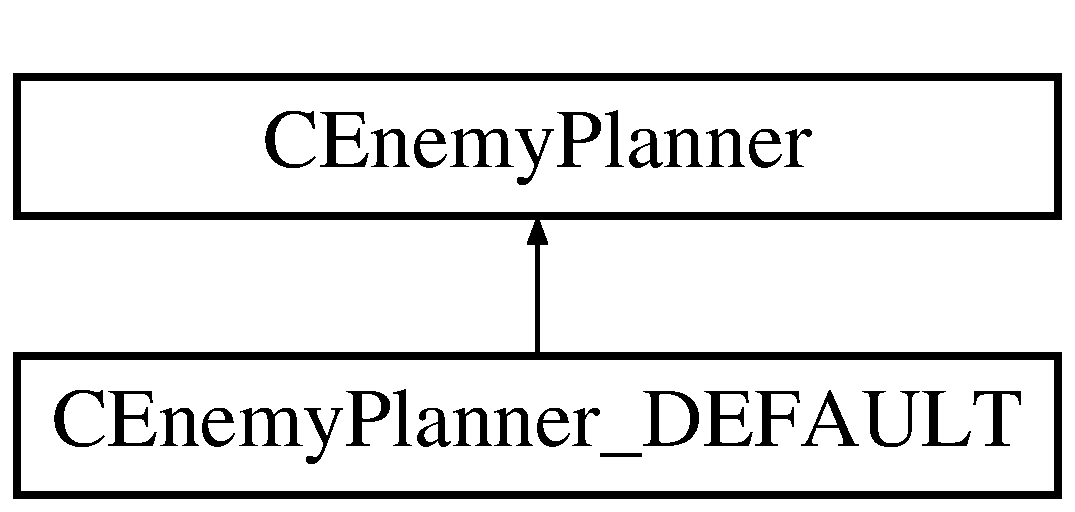
\includegraphics[height=2.000000cm]{class_c_enemy_planner___d_e_f_a_u_l_t}
\end{center}
\end{figure}
\subsection*{Public Member Functions}
\begin{DoxyCompactItemize}
\item 
{\bfseries C\+Enemy\+Planner\+\_\+\+D\+E\+F\+A\+U\+LT} (std\+::string \+\_\+name)\hypertarget{class_c_enemy_planner___d_e_f_a_u_l_t_ae95fc05ddfd1e98343c3feff51578153}{}\label{class_c_enemy_planner___d_e_f_a_u_l_t_ae95fc05ddfd1e98343c3feff51578153}

\item 
int {\bfseries Get\+Plan} (const \hyperlink{class_c_enemy}{C\+Enemy} $\ast$\+\_\+enemy)\hypertarget{class_c_enemy_planner___d_e_f_a_u_l_t_a7e5c3c4b12842793c429d6a2d08c824d}{}\label{class_c_enemy_planner___d_e_f_a_u_l_t_a7e5c3c4b12842793c429d6a2d08c824d}

\end{DoxyCompactItemize}
\subsection*{Additional Inherited Members}


The documentation for this class was generated from the following files\+:\begin{DoxyCompactItemize}
\item 
Classes/Enemy\+Planner.\+h\item 
Classes/Enemy\+Planner.\+cpp\end{DoxyCompactItemize}

\hypertarget{class_c_enemy_planner___m_y_h_p}{}\section{C\+Enemy\+Planner\+\_\+\+M\+Y\+HP Class Reference}
\label{class_c_enemy_planner___m_y_h_p}\index{C\+Enemy\+Planner\+\_\+\+M\+Y\+HP@{C\+Enemy\+Planner\+\_\+\+M\+Y\+HP}}
Inheritance diagram for C\+Enemy\+Planner\+\_\+\+M\+Y\+HP\+:\begin{figure}[H]
\begin{center}
\leavevmode
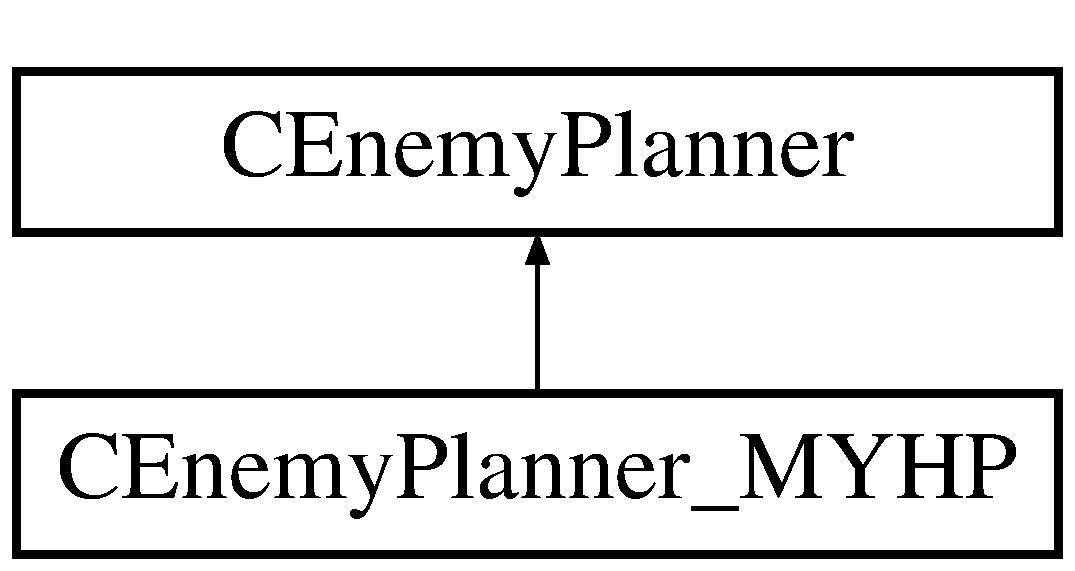
\includegraphics[height=2.000000cm]{class_c_enemy_planner___m_y_h_p}
\end{center}
\end{figure}
\subsection*{Public Member Functions}
\begin{DoxyCompactItemize}
\item 
{\bfseries C\+Enemy\+Planner\+\_\+\+M\+Y\+HP} (std\+::string \+\_\+name, std\+::vector$<$ std\+::string $>$ \+\_\+arg\+List)\hypertarget{class_c_enemy_planner___m_y_h_p_afe0ecb2d463f28d5db23f5aed233a1c0}{}\label{class_c_enemy_planner___m_y_h_p_afe0ecb2d463f28d5db23f5aed233a1c0}

\item 
int {\bfseries Get\+Plan} (const \hyperlink{class_c_enemy}{C\+Enemy} $\ast$\+\_\+enemy)\hypertarget{class_c_enemy_planner___m_y_h_p_a274c0f95bcdf2539f011f323a6241cdd}{}\label{class_c_enemy_planner___m_y_h_p_a274c0f95bcdf2539f011f323a6241cdd}

\end{DoxyCompactItemize}
\subsection*{Additional Inherited Members}


The documentation for this class was generated from the following files\+:\begin{DoxyCompactItemize}
\item 
Classes/Enemy\+Planner.\+h\item 
Classes/Enemy\+Planner.\+cpp\end{DoxyCompactItemize}

\hypertarget{class_c_enemy_planner___p_l_a_y_e_r_n_u_m}{}\section{C\+Enemy\+Planner\+\_\+\+P\+L\+A\+Y\+E\+R\+N\+UM Class Reference}
\label{class_c_enemy_planner___p_l_a_y_e_r_n_u_m}\index{C\+Enemy\+Planner\+\_\+\+P\+L\+A\+Y\+E\+R\+N\+UM@{C\+Enemy\+Planner\+\_\+\+P\+L\+A\+Y\+E\+R\+N\+UM}}
Inheritance diagram for C\+Enemy\+Planner\+\_\+\+P\+L\+A\+Y\+E\+R\+N\+UM\+:\begin{figure}[H]
\begin{center}
\leavevmode
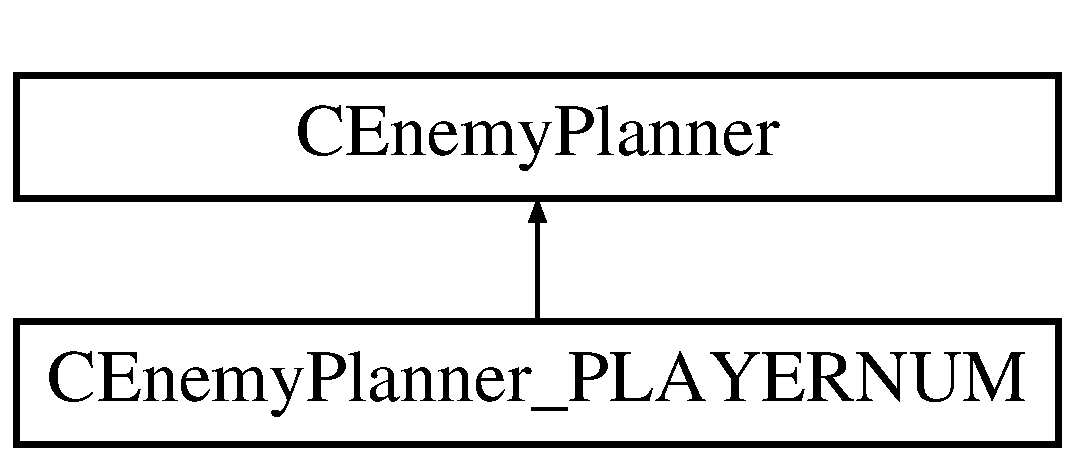
\includegraphics[height=2.000000cm]{class_c_enemy_planner___p_l_a_y_e_r_n_u_m}
\end{center}
\end{figure}
\subsection*{Public Member Functions}
\begin{DoxyCompactItemize}
\item 
{\bfseries C\+Enemy\+Planner\+\_\+\+P\+L\+A\+Y\+E\+R\+N\+UM} (std\+::string \+\_\+name, std\+::vector$<$ std\+::string $>$ \+\_\+arg\+List)\hypertarget{class_c_enemy_planner___p_l_a_y_e_r_n_u_m_a1168d5a04a097ce0747914ce9eaf65e1}{}\label{class_c_enemy_planner___p_l_a_y_e_r_n_u_m_a1168d5a04a097ce0747914ce9eaf65e1}

\item 
int {\bfseries Get\+Plan} (const \hyperlink{class_c_enemy}{C\+Enemy} $\ast$\+\_\+enemy)\hypertarget{class_c_enemy_planner___p_l_a_y_e_r_n_u_m_ae3b0858481479ba5ac8a3e7adec5d5ab}{}\label{class_c_enemy_planner___p_l_a_y_e_r_n_u_m_ae3b0858481479ba5ac8a3e7adec5d5ab}

\end{DoxyCompactItemize}
\subsection*{Additional Inherited Members}


The documentation for this class was generated from the following files\+:\begin{DoxyCompactItemize}
\item 
Classes/Enemy\+Planner.\+h\item 
Classes/Enemy\+Planner.\+cpp\end{DoxyCompactItemize}

\hypertarget{class_c_enemy_species}{}\section{C\+Enemy\+Species Class Reference}
\label{class_c_enemy_species}\index{C\+Enemy\+Species@{C\+Enemy\+Species}}
Inheritance diagram for C\+Enemy\+Species\+:\begin{figure}[H]
\begin{center}
\leavevmode
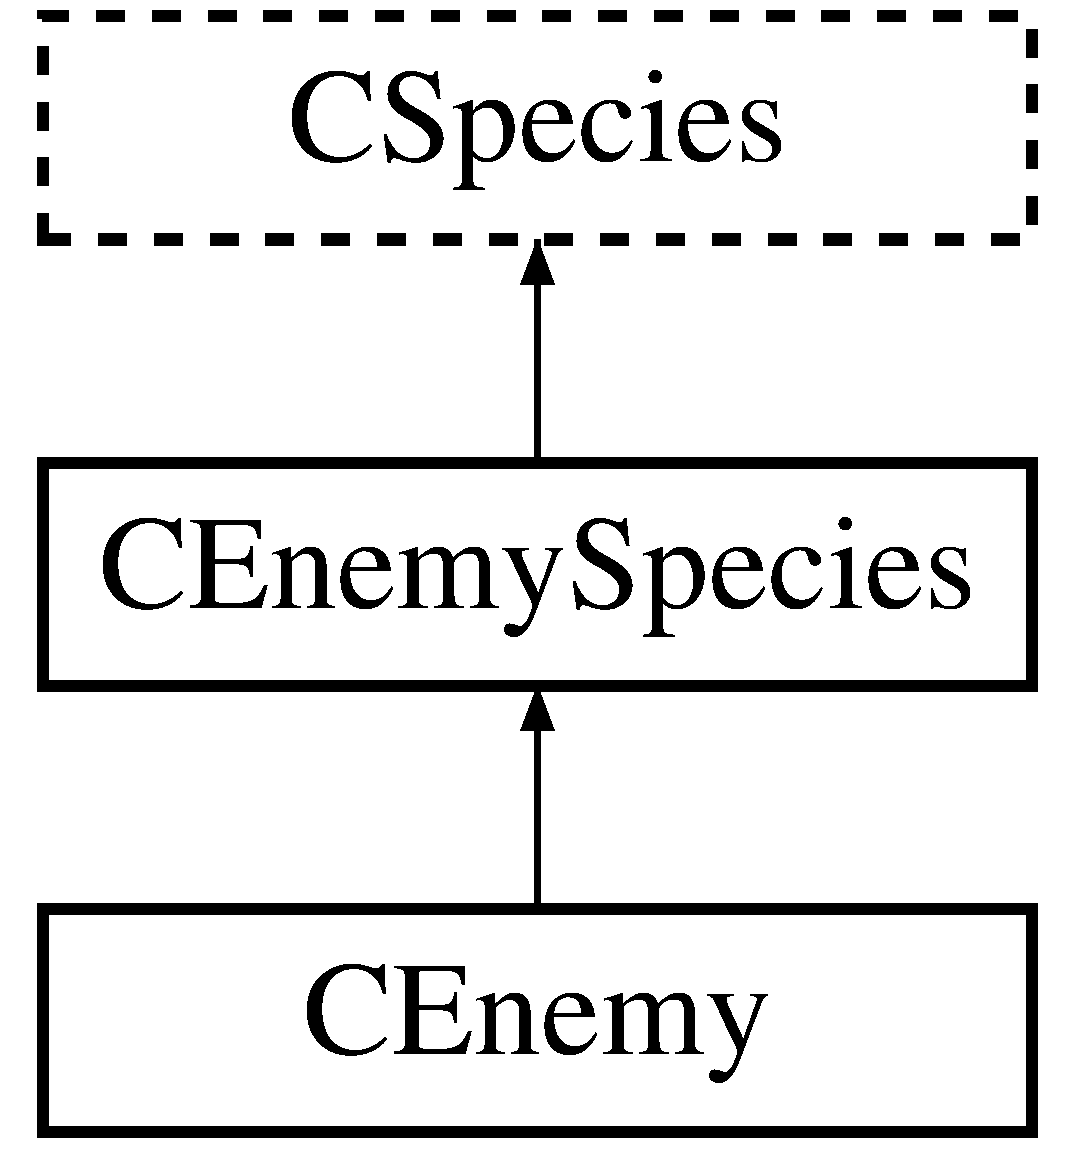
\includegraphics[height=3.000000cm]{class_c_enemy_species}
\end{center}
\end{figure}
\subsection*{Public Member Functions}
\begin{DoxyCompactItemize}
\item 
{\bfseries C\+Enemy\+Species} (const \hyperlink{class_c_enemy_species}{C\+Enemy\+Species} \&obj)\hypertarget{class_c_enemy_species_a50bb7bb336aefc6ebbc76aa0232261e4}{}\label{class_c_enemy_species_a50bb7bb336aefc6ebbc76aa0232261e4}

\item 
int {\bfseries Get\+Gold\+Gene} ()\hypertarget{class_c_enemy_species_a88758588bd7f6125ae12a4b1ed2a2705}{}\label{class_c_enemy_species_a88758588bd7f6125ae12a4b1ed2a2705}

\item 
int {\bfseries Get\+Exp\+Gene} ()\hypertarget{class_c_enemy_species_a2c160eaf598214093a78302b8c6bc663}{}\label{class_c_enemy_species_a2c160eaf598214093a78302b8c6bc663}

\end{DoxyCompactItemize}
\subsection*{Protected Attributes}
\begin{DoxyCompactItemize}
\item 
\hyperlink{class_c_enemy_a_i}{C\+Enemy\+AI} {\bfseries AI}\hypertarget{class_c_enemy_species_ab762c44a7e2d33bc3a7137d9f160f654}{}\label{class_c_enemy_species_ab762c44a7e2d33bc3a7137d9f160f654}

\item 
std\+::vector$<$ std\+::pair$<$ std\+::string, int $>$ $>$ {\bfseries Drop\+Item\+List}\hypertarget{class_c_enemy_species_ad24c8add86987bc70da6f2e6790b6851}{}\label{class_c_enemy_species_ad24c8add86987bc70da6f2e6790b6851}

\item 
int {\bfseries Gold\+Gene}\hypertarget{class_c_enemy_species_a31978d7b6ff2e0005e17ae18b52fb609}{}\label{class_c_enemy_species_a31978d7b6ff2e0005e17ae18b52fb609}

\item 
int {\bfseries Exp\+Gene}\hypertarget{class_c_enemy_species_a45710208ef330a71c7924c96ca308fc3}{}\label{class_c_enemy_species_a45710208ef330a71c7924c96ca308fc3}

\end{DoxyCompactItemize}
\subsection*{Friends}
\begin{DoxyCompactItemize}
\item 
class {\bfseries C\+Enemy\+Species\+Manager}\hypertarget{class_c_enemy_species_a0789d2c1309cbdcb1f1095c865b9312e}{}\label{class_c_enemy_species_a0789d2c1309cbdcb1f1095c865b9312e}

\end{DoxyCompactItemize}
\subsection*{Additional Inherited Members}


The documentation for this class was generated from the following file\+:\begin{DoxyCompactItemize}
\item 
Classes/Species.\+h\end{DoxyCompactItemize}

\hypertarget{class_c_enemy_species_manager}{}\section{C\+Enemy\+Species\+Manager Class Reference}
\label{class_c_enemy_species_manager}\index{C\+Enemy\+Species\+Manager@{C\+Enemy\+Species\+Manager}}
\subsection*{Public Member Functions}
\begin{DoxyCompactItemize}
\item 
void {\bfseries Clear} ()\hypertarget{class_c_enemy_species_manager_a61bff3c97ea2615e6f212f8fd90f2cbd}{}\label{class_c_enemy_species_manager_a61bff3c97ea2615e6f212f8fd90f2cbd}

\item 
bool {\bfseries Create\+Species} (const char $\ast$\+\_\+name, int \+\_\+level, int \+\_\+gene\+Max\+Hp, int \+\_\+gene\+Atk, int \+\_\+gene\+Def, int \+\_\+gene\+Spd, int \+\_\+img)\hypertarget{class_c_enemy_species_manager_a075696984dd79e5243239ecfcb088696}{}\label{class_c_enemy_species_manager_a075696984dd79e5243239ecfcb088696}

\item 
bool {\bfseries Set\+Trick\+List} (const char $\ast$\+\_\+name, std\+::vector$<$ \hyperlink{structtrick__tag}{trick\+\_\+tag} const $\ast$ $>$ \+\_\+trick\+List)\hypertarget{class_c_enemy_species_manager_aa73abd6d351d50a114ddb745733f99ab}{}\label{class_c_enemy_species_manager_aa73abd6d351d50a114ddb745733f99ab}

\item 
bool {\bfseries Set\+Drop\+Item\+List} (const char $\ast$\+\_\+name, std\+::vector$<$ std\+::pair$<$ std\+::string, int $>$ $>$ \+\_\+drop\+Item\+List)\hypertarget{class_c_enemy_species_manager_a62f78b19892fb446413109e1e491f698}{}\label{class_c_enemy_species_manager_a62f78b19892fb446413109e1e491f698}

\item 
bool {\bfseries Add\+Random\+Plan\+Set} (const char $\ast$\+\_\+name, unsigned int \+\_\+index, std\+::vector$<$ std\+::pair$<$ int, int $>$ $>$ \+\_\+plan\+List, bool \+\_\+default\+Plan=false)\hypertarget{class_c_enemy_species_manager_ae885e38198c0920abf4b94dd8aaa4493}{}\label{class_c_enemy_species_manager_ae885e38198c0920abf4b94dd8aaa4493}

\item 
bool {\bfseries Set\+Enemy\+Planner} (std\+::string \+\_\+enemy\+Name, std\+::string \+\_\+type\+Name, std\+::vector$<$ std\+::string $>$ \+\_\+arg\+List)\hypertarget{class_c_enemy_species_manager_a5bd6ed0db0ae0ae3c730da688c99ca07}{}\label{class_c_enemy_species_manager_a5bd6ed0db0ae0ae3c730da688c99ca07}

\item 
bool {\bfseries Set\+Enemy\+Targetter} (std\+::string \+\_\+enemy\+Name, std\+::string \+\_\+type\+Name, std\+::vector$<$ std\+::string $>$ \+\_\+arg\+List)\hypertarget{class_c_enemy_species_manager_a797a72318055c9ae74acba4feb86cbfb}{}\label{class_c_enemy_species_manager_a797a72318055c9ae74acba4feb86cbfb}

\item 
\hyperlink{class_c_enemy_species}{C\+Enemy\+Species} $\ast$ {\bfseries Get\+Species} (const char $\ast$\+\_\+name)\hypertarget{class_c_enemy_species_manager_af0a736cc0fdb58408b900667871ae5c1}{}\label{class_c_enemy_species_manager_af0a736cc0fdb58408b900667871ae5c1}

\item 
bool {\bfseries Set\+Map\+Encount} (int \+\_\+mapnum, int \+\_\+chipnum, int \+\_\+encount)\hypertarget{class_c_enemy_species_manager_a01147031a924bdf6ed939829b7e69084}{}\label{class_c_enemy_species_manager_a01147031a924bdf6ed939829b7e69084}

\item 
bool {\bfseries Add\+Map\+Encount\+Party} (int \+\_\+mapnum, int \+\_\+chipnum, int \+\_\+encount, std\+::vector$<$ std\+::string $>$ \+\_\+party)\hypertarget{class_c_enemy_species_manager_aeda3ed33dc2cda2139c9642e78be6488}{}\label{class_c_enemy_species_manager_aeda3ed33dc2cda2139c9642e78be6488}

\item 
bool {\bfseries Check\+Encount} (int \+\_\+mapnum, int \+\_\+chipnum, std\+::vector$<$ \hyperlink{class_c_enemy_species}{C\+Enemy\+Species} $\ast$ $>$ \&\+\_\+party\+\_\+p)\hypertarget{class_c_enemy_species_manager_aa81ecf36891b968c3723b3e635b97059}{}\label{class_c_enemy_species_manager_aa81ecf36891b968c3723b3e635b97059}

\item 
bool {\bfseries Check\+After\+Load} ()\hypertarget{class_c_enemy_species_manager_a1a5a8d5c7486a3e25736283c13bbe5c7}{}\label{class_c_enemy_species_manager_a1a5a8d5c7486a3e25736283c13bbe5c7}

\end{DoxyCompactItemize}
\subsection*{Static Public Member Functions}
\begin{DoxyCompactItemize}
\item 
static \hyperlink{class_c_enemy_species_manager}{C\+Enemy\+Species\+Manager} $\ast$ {\bfseries Get\+Instance} ()\hypertarget{class_c_enemy_species_manager_a0b12e5c3c55fdd368aed2d475a7f9a47}{}\label{class_c_enemy_species_manager_a0b12e5c3c55fdd368aed2d475a7f9a47}

\end{DoxyCompactItemize}


The documentation for this class was generated from the following files\+:\begin{DoxyCompactItemize}
\item 
Classes/Enemy\+Species\+Manager.\+h\item 
Classes/Enemy\+Species\+Manager.\+cpp\end{DoxyCompactItemize}

\hypertarget{class_c_enemy_targetter}{}\section{C\+Enemy\+Targetter Class Reference}
\label{class_c_enemy_targetter}\index{C\+Enemy\+Targetter@{C\+Enemy\+Targetter}}
Inheritance diagram for C\+Enemy\+Targetter\+:\begin{figure}[H]
\begin{center}
\leavevmode
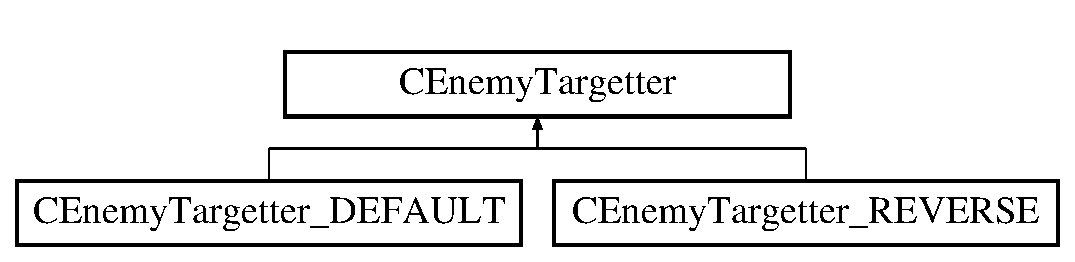
\includegraphics[height=2.000000cm]{class_c_enemy_targetter}
\end{center}
\end{figure}
\subsection*{Public Member Functions}
\begin{DoxyCompactItemize}
\item 
{\bfseries C\+Enemy\+Targetter} (std\+::string \+\_\+enemyname)\hypertarget{class_c_enemy_targetter_a7ecc3fbd1e11b6d8d7c20f23edc9e67e}{}\label{class_c_enemy_targetter_a7ecc3fbd1e11b6d8d7c20f23edc9e67e}

\item 
void {\bfseries Battle\+Ready} (const \hyperlink{class_c_actor}{C\+Actor} $\ast$const $\ast$\+\_\+actor\+List, const int \+\_\+player\+Num, const int \+\_\+enemy\+Num)\hypertarget{class_c_enemy_targetter_a7a806237d0572e0e99d7436f490819e4}{}\label{class_c_enemy_targetter_a7a806237d0572e0e99d7436f490819e4}

\item 
void {\bfseries Set\+Attention} (int \+\_\+attention\mbox{[}$\,$\mbox{]})\hypertarget{class_c_enemy_targetter_a78335cd359e3354d60068348c2853e33}{}\label{class_c_enemy_targetter_a78335cd359e3354d60068348c2853e33}

\item 
std\+::string {\bfseries Get\+Name} () const \hypertarget{class_c_enemy_targetter_a464d9e107f03ac604878cafb71b62636}{}\label{class_c_enemy_targetter_a464d9e107f03ac604878cafb71b62636}

\item 
virtual int {\bfseries Get\+Target} (const \hyperlink{class_c_enemy}{C\+Enemy} $\ast$\+\_\+enemy)=0\hypertarget{class_c_enemy_targetter_af1224ba428b8ec538c665be65c3821e6}{}\label{class_c_enemy_targetter_af1224ba428b8ec538c665be65c3821e6}

\item 
void {\bfseries Calc\+Attention\+Rank} ()\hypertarget{class_c_enemy_targetter_a71cd33e88d6775738e76ed87d2399465}{}\label{class_c_enemy_targetter_a71cd33e88d6775738e76ed87d2399465}

\item 
int {\bfseries Get\+Attention\+Rank} (int \+\_\+key)\hypertarget{class_c_enemy_targetter_a59a3f4ace2840d37aa7559e08d312c58}{}\label{class_c_enemy_targetter_a59a3f4ace2840d37aa7559e08d312c58}

\end{DoxyCompactItemize}
\subsection*{Protected Attributes}
\begin{DoxyCompactItemize}
\item 
const \hyperlink{class_c_actor}{C\+Actor} $\ast$const $\ast$ {\bfseries Actor}\hypertarget{class_c_enemy_targetter_a0a9807c1bae91f90e2648e25905f70a8}{}\label{class_c_enemy_targetter_a0a9807c1bae91f90e2648e25905f70a8}

\item 
int {\bfseries P\+L\+A\+Y\+E\+R\+\_\+\+N\+UM}\hypertarget{class_c_enemy_targetter_abba63cf970c8452e637a5666c84795de}{}\label{class_c_enemy_targetter_abba63cf970c8452e637a5666c84795de}

\item 
int {\bfseries E\+N\+E\+M\+Y\+\_\+\+N\+UM}\hypertarget{class_c_enemy_targetter_ab53b98698c5e32c78c58cf2bc070316c}{}\label{class_c_enemy_targetter_ab53b98698c5e32c78c58cf2bc070316c}

\end{DoxyCompactItemize}
\subsection*{Static Protected Attributes}
\begin{DoxyCompactItemize}
\item 
static const int {\bfseries A\+T\+T\+E\+N\+T\+I\+O\+N\+\_\+\+R\+A\+T\+IO} \mbox{[}M\+A\+X\+\_\+\+P\+L\+A\+Y\+E\+R\+\_\+\+N\+UM\mbox{]} = \{4, 2, 1\}\hypertarget{class_c_enemy_targetter_a7b84c79982d75a00756e6f01ef56743b}{}\label{class_c_enemy_targetter_a7b84c79982d75a00756e6f01ef56743b}

\end{DoxyCompactItemize}


The documentation for this class was generated from the following files\+:\begin{DoxyCompactItemize}
\item 
Classes/Enemy\+Targetter.\+h\item 
Classes/Enemy\+Targetter.\+cpp\end{DoxyCompactItemize}

\hypertarget{class_c_enemy_targetter___d_e_f_a_u_l_t}{}\section{C\+Enemy\+Targetter\+\_\+\+D\+E\+F\+A\+U\+LT Class Reference}
\label{class_c_enemy_targetter___d_e_f_a_u_l_t}\index{C\+Enemy\+Targetter\+\_\+\+D\+E\+F\+A\+U\+LT@{C\+Enemy\+Targetter\+\_\+\+D\+E\+F\+A\+U\+LT}}
Inheritance diagram for C\+Enemy\+Targetter\+\_\+\+D\+E\+F\+A\+U\+LT\+:\begin{figure}[H]
\begin{center}
\leavevmode
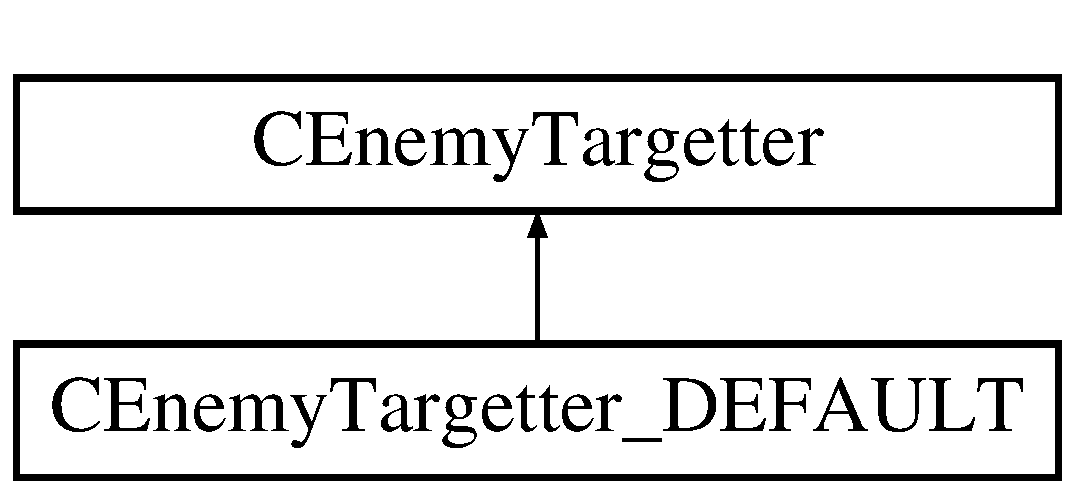
\includegraphics[height=2.000000cm]{class_c_enemy_targetter___d_e_f_a_u_l_t}
\end{center}
\end{figure}
\subsection*{Public Member Functions}
\begin{DoxyCompactItemize}
\item 
{\bfseries C\+Enemy\+Targetter\+\_\+\+D\+E\+F\+A\+U\+LT} (std\+::string \+\_\+name)\hypertarget{class_c_enemy_targetter___d_e_f_a_u_l_t_a09151e2d1fdcafb13695fbdaf4ddb0d6}{}\label{class_c_enemy_targetter___d_e_f_a_u_l_t_a09151e2d1fdcafb13695fbdaf4ddb0d6}

\item 
int {\bfseries Get\+Target} (const \hyperlink{class_c_enemy}{C\+Enemy} $\ast$\+\_\+enemy)\hypertarget{class_c_enemy_targetter___d_e_f_a_u_l_t_a221751274c2f19743d340efded294cd7}{}\label{class_c_enemy_targetter___d_e_f_a_u_l_t_a221751274c2f19743d340efded294cd7}

\end{DoxyCompactItemize}
\subsection*{Additional Inherited Members}


The documentation for this class was generated from the following files\+:\begin{DoxyCompactItemize}
\item 
Classes/Enemy\+Targetter.\+h\item 
Classes/Enemy\+Targetter.\+cpp\end{DoxyCompactItemize}

\hypertarget{class_c_enemy_targetter___r_e_v_e_r_s_e}{}\section{C\+Enemy\+Targetter\+\_\+\+R\+E\+V\+E\+R\+SE Class Reference}
\label{class_c_enemy_targetter___r_e_v_e_r_s_e}\index{C\+Enemy\+Targetter\+\_\+\+R\+E\+V\+E\+R\+SE@{C\+Enemy\+Targetter\+\_\+\+R\+E\+V\+E\+R\+SE}}
Inheritance diagram for C\+Enemy\+Targetter\+\_\+\+R\+E\+V\+E\+R\+SE\+:\begin{figure}[H]
\begin{center}
\leavevmode
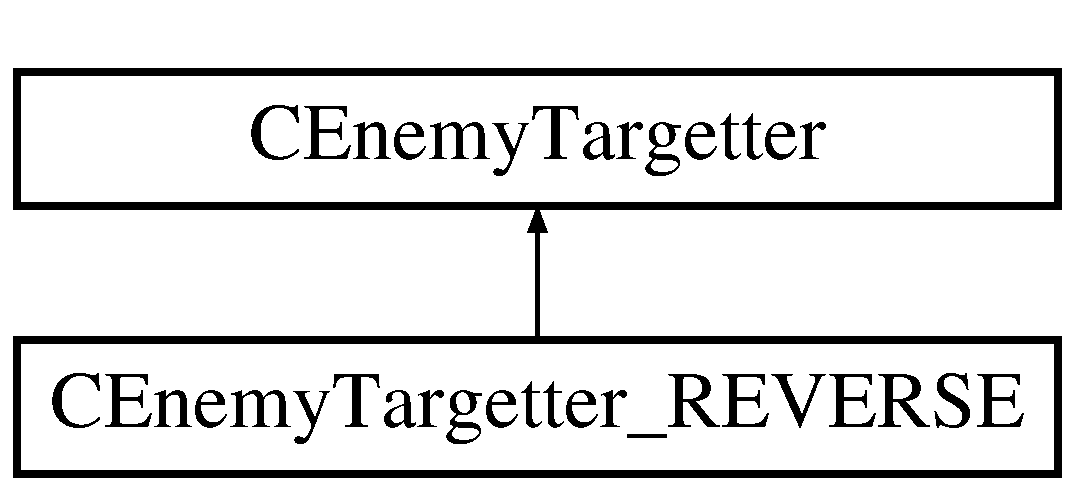
\includegraphics[height=2.000000cm]{class_c_enemy_targetter___r_e_v_e_r_s_e}
\end{center}
\end{figure}
\subsection*{Public Member Functions}
\begin{DoxyCompactItemize}
\item 
{\bfseries C\+Enemy\+Targetter\+\_\+\+R\+E\+V\+E\+R\+SE} (std\+::string \+\_\+name)\hypertarget{class_c_enemy_targetter___r_e_v_e_r_s_e_ad0098a6d5d0b7a5f05d2278605ec6134}{}\label{class_c_enemy_targetter___r_e_v_e_r_s_e_ad0098a6d5d0b7a5f05d2278605ec6134}

\item 
int {\bfseries Get\+Target} (const \hyperlink{class_c_enemy}{C\+Enemy} $\ast$\+\_\+enemy)\hypertarget{class_c_enemy_targetter___r_e_v_e_r_s_e_af94f5109663093ba6804382f5c42c057}{}\label{class_c_enemy_targetter___r_e_v_e_r_s_e_af94f5109663093ba6804382f5c42c057}

\end{DoxyCompactItemize}
\subsection*{Additional Inherited Members}


The documentation for this class was generated from the following files\+:\begin{DoxyCompactItemize}
\item 
Classes/Enemy\+Targetter.\+h\item 
Classes/Enemy\+Targetter.\+cpp\end{DoxyCompactItemize}

\hypertarget{class_c_eve_manager}{}\section{C\+Eve\+Manager Class Reference}
\label{class_c_eve_manager}\index{C\+Eve\+Manager@{C\+Eve\+Manager}}
\subsection*{Public Member Functions}
\begin{DoxyCompactItemize}
\item 
void {\bfseries Init} ()\hypertarget{class_c_eve_manager_a81b830f9b23ebba1e077c3e47f72f0f6}{}\label{class_c_eve_manager_a81b830f9b23ebba1e077c3e47f72f0f6}

\item 
void {\bfseries Save} (F\+I\+LE $\ast$fp)\hypertarget{class_c_eve_manager_adb2b8e538af22ca621a6287cf838ab9b}{}\label{class_c_eve_manager_adb2b8e538af22ca621a6287cf838ab9b}

\item 
void {\bfseries Draw} (int \+\_\+mapnum, int \+\_\+x, int \+\_\+y, bool \+\_\+overdraw=false, int \+\_\+dx=0, int \+\_\+dy=0)\hypertarget{class_c_eve_manager_a6fab97f20090b6151b8bae156468000f}{}\label{class_c_eve_manager_a6fab97f20090b6151b8bae156468000f}

\item 
void {\bfseries Set\+Map} (unsigned int \+\_\+mapnum, int \+\_\+filesize, unsigned char $\ast$buf)\hypertarget{class_c_eve_manager_a31457fdd1db1d4a1dd57a6d9e125b1ee}{}\label{class_c_eve_manager_a31457fdd1db1d4a1dd57a6d9e125b1ee}

\item 
void {\bfseries Set\+Eve\+Obj} (int \+\_\+mapnum, int \+\_\+datanum, int \+\_\+kind, int \+\_\+img\mbox{[}C\+H\+A\+R\+A\+\_\+\+P\+I\+C\+\_\+\+N\+UM\mbox{]}, const char $\ast$\+\_\+pickey, char $\ast$\+\_\+name, bool \+\_\+visible)\hypertarget{class_c_eve_manager_a2d31d0d756b85416f121ff94b0715352}{}\label{class_c_eve_manager_a2d31d0d756b85416f121ff94b0715352}

\item 
void {\bfseries Set\+Position} (const char $\ast$\+\_\+name, int \+\_\+dx, int \+\_\+dy, bool \+\_\+d=false)\hypertarget{class_c_eve_manager_a5abb9c13b74f5597e7598513cedc7248}{}\label{class_c_eve_manager_a5abb9c13b74f5597e7598513cedc7248}

\item 
void {\bfseries Set\+Position} (const char $\ast$\+\_\+name, const char $\ast$\+\_\+targetname)\hypertarget{class_c_eve_manager_a26d64a722dfc2f65a1b6d0d30c20d2f5}{}\label{class_c_eve_manager_a26d64a722dfc2f65a1b6d0d30c20d2f5}

\item 
void {\bfseries Set\+Position} (const char $\ast$\+\_\+name, int \+\_\+datanum)\hypertarget{class_c_eve_manager_a0c404d20b62870073c652eb068f0ea76}{}\label{class_c_eve_manager_a0c404d20b62870073c652eb068f0ea76}

\item 
void {\bfseries Set\+Pic} (const char $\ast$\+\_\+name, const int \+\_\+img\mbox{[}C\+H\+A\+R\+A\+\_\+\+P\+I\+C\+\_\+\+N\+UM\mbox{]}, const char $\ast$\+\_\+pickey)\hypertarget{class_c_eve_manager_ab06d15c3d24c0f375f2f0fbf7c93a09a}{}\label{class_c_eve_manager_ab06d15c3d24c0f375f2f0fbf7c93a09a}

\item 
bool {\bfseries Get\+Pos} (const char $\ast$\+\_\+name, int $\ast$\+\_\+mapnum, int $\ast$\+\_\+x, int $\ast$\+\_\+y)\hypertarget{class_c_eve_manager_aaab5f2af51e52e321820aaa5899b3f42}{}\label{class_c_eve_manager_aaab5f2af51e52e321820aaa5899b3f42}

\item 
bool {\bfseries Get\+Pos} (const int \+\_\+mapnum, const int \+\_\+datanum, int $\ast$\+\_\+x, int $\ast$\+\_\+y)\hypertarget{class_c_eve_manager_a3d261065c2a87a8f30c358e307a55343}{}\label{class_c_eve_manager_a3d261065c2a87a8f30c358e307a55343}

\item 
bool {\bfseries Get\+Text} (char $\ast$$\ast$\&\+\_\+text, int \&\+\_\+count, int \+\_\+mapnum, int \+\_\+x, int \+\_\+y, int \+\_\+mydir, int \+\_\+kind=-\/1)\hypertarget{class_c_eve_manager_a2c4dbfe9aad0101b96b5fb0e8bc80ee7}{}\label{class_c_eve_manager_a2c4dbfe9aad0101b96b5fb0e8bc80ee7}

\item 
void {\bfseries Set\+Text} (const char \+\_\+eventtext\mbox{[}1000\mbox{]}\mbox{[}256\mbox{]}, const int \+\_\+line, const char $\ast$\+\_\+name, const int \+\_\+kind)\hypertarget{class_c_eve_manager_ae0fad035cbcdb2e78aa519f3f26e1e98}{}\label{class_c_eve_manager_ae0fad035cbcdb2e78aa519f3f26e1e98}

\item 
bool {\bfseries Copy\+Original\+Event} (std\+::vector$<$ \hyperlink{structchar256}{char256} $>$ $\ast$vectext\+\_\+p, const char $\ast$\+\_\+eventtext, int \+\_\+count=0)\hypertarget{class_c_eve_manager_ada2ae4db5f86e66f5dda8e5077d59754}{}\label{class_c_eve_manager_ada2ae4db5f86e66f5dda8e5077d59754}

\item 
bool {\bfseries Check\+Walkable} (int \+\_\+mapnum, int \+\_\+x, int \+\_\+y)\hypertarget{class_c_eve_manager_aabd1190c4380d0c76cfe6669de019c28}{}\label{class_c_eve_manager_aabd1190c4380d0c76cfe6669de019c28}

\item 
void {\bfseries Set\+Dir} (const char $\ast$\+\_\+name, int \+\_\+dir)\hypertarget{class_c_eve_manager_afbb09f19a49e852dd157d32ab19ab9c6}{}\label{class_c_eve_manager_afbb09f19a49e852dd157d32ab19ab9c6}

\item 
void {\bfseries Set\+Visible} (const char $\ast$\+\_\+name, bool \+\_\+visible)\hypertarget{class_c_eve_manager_ad6f39f63d16bf738574168fc013d7163}{}\label{class_c_eve_manager_ad6f39f63d16bf738574168fc013d7163}

\item 
void {\bfseries Set\+Alpha} (const char $\ast$\+\_\+name, unsigned char \+\_\+alpha)\hypertarget{class_c_eve_manager_a429c6f79450735dee4b975d629b9d63d}{}\label{class_c_eve_manager_a429c6f79450735dee4b975d629b9d63d}

\item 
void {\bfseries Set\+Effect} (const char $\ast$\+\_\+name, int \+\_\+effectname, int \+\_\+effectnum\mbox{[}$\,$\mbox{]})\hypertarget{class_c_eve_manager_aa337fab7ca7e0e3b3c307482800525ee}{}\label{class_c_eve_manager_aa337fab7ca7e0e3b3c307482800525ee}

\item 
void {\bfseries Set\+Count} (const char $\ast$\+\_\+name, int \+\_\+count, bool \+\_\+add=false)\hypertarget{class_c_eve_manager_a88e81c11881a8caf7ba980f5618c79cc}{}\label{class_c_eve_manager_a88e81c11881a8caf7ba980f5618c79cc}

\item 
void {\bfseries Set\+Now\+Name} (const char $\ast$\+\_\+name)\hypertarget{class_c_eve_manager_aa384e6fb4831d74d3ad32e5c52e01c03}{}\label{class_c_eve_manager_aa384e6fb4831d74d3ad32e5c52e01c03}

\item 
void {\bfseries Jump} (\hyperlink{class_c_field}{C\+Field} $\ast$\+\_\+field, char $\ast$\+\_\+name)\hypertarget{class_c_eve_manager_a5100c61ddc22f44a7d8e34545e86d48b}{}\label{class_c_eve_manager_a5100c61ddc22f44a7d8e34545e86d48b}

\item 
void {\bfseries Walk} (\hyperlink{class_c_field}{C\+Field} $\ast$\+\_\+field, char $\ast$\+\_\+name, int \+\_\+dir, int \+\_\+walkspeed, bool \+\_\+walk=true, int \+\_\+fade=0)\hypertarget{class_c_eve_manager_af9bb4ce19f480ad4a0fd7921b86d4aaf}{}\label{class_c_eve_manager_af9bb4ce19f480ad4a0fd7921b86d4aaf}

\end{DoxyCompactItemize}
\subsection*{Static Public Member Functions}
\begin{DoxyCompactItemize}
\item 
static \hyperlink{class_c_eve_manager}{C\+Eve\+Manager} $\ast$ {\bfseries Get\+Instance} ()\hypertarget{class_c_eve_manager_ae2b6a37be91de68fc22778eea00ad71a}{}\label{class_c_eve_manager_ae2b6a37be91de68fc22778eea00ad71a}

\end{DoxyCompactItemize}


The documentation for this class was generated from the following files\+:\begin{DoxyCompactItemize}
\item 
Classes/Eve\+Manager.\+h\item 
Classes/Eve\+Manager.\+cpp\end{DoxyCompactItemize}

\hypertarget{class_c_eve_obj}{}\section{C\+Eve\+Obj Class Reference}
\label{class_c_eve_obj}\index{C\+Eve\+Obj@{C\+Eve\+Obj}}
\subsection*{Public Member Functions}
\begin{DoxyCompactItemize}
\item 
{\bfseries C\+Eve\+Obj} (unsigned char \+\_\+datanum=0)\hypertarget{class_c_eve_obj_a25c68cb9fa77435cef1fb063b47d6230}{}\label{class_c_eve_obj_a25c68cb9fa77435cef1fb063b47d6230}

\item 
void {\bfseries Draw} (int \+\_\+x, int \+\_\+y)\hypertarget{class_c_eve_obj_a46c8ef453357ea0299483afe1d96f329}{}\label{class_c_eve_obj_a46c8ef453357ea0299483afe1d96f329}

\end{DoxyCompactItemize}
\subsection*{Public Attributes}
\begin{DoxyCompactItemize}
\item 
unsigned int {\bfseries Mapnum}\hypertarget{class_c_eve_obj_a25a6a77a2177ecac2d200d20efbb4e0a}{}\label{class_c_eve_obj_a25a6a77a2177ecac2d200d20efbb4e0a}

\item 
unsigned char {\bfseries Datanum}\hypertarget{class_c_eve_obj_a0922ab84ee288549ac53dc727e1d1474}{}\label{class_c_eve_obj_a0922ab84ee288549ac53dc727e1d1474}

\item 
char {\bfseries Name} \mbox{[}32\mbox{]}\hypertarget{class_c_eve_obj_a9c25c04d1db6c83c2f1b6732be8fadee}{}\label{class_c_eve_obj_a9c25c04d1db6c83c2f1b6732be8fadee}

\item 
std\+::vector$<$ \hyperlink{structchar256}{char256} $>$ {\bfseries Text}\hypertarget{class_c_eve_obj_aaf99720b5406ed50ccb237228b32b077}{}\label{class_c_eve_obj_aaf99720b5406ed50ccb237228b32b077}

\item 
int {\bfseries Count}\hypertarget{class_c_eve_obj_ac9e0643f647e960e1717633671d0e318}{}\label{class_c_eve_obj_ac9e0643f647e960e1717633671d0e318}

\item 
int {\bfseries Img} \mbox{[}C\+H\+A\+R\+A\+\_\+\+P\+I\+C\+\_\+\+N\+UM\mbox{]}\hypertarget{class_c_eve_obj_ae4889e89b5fcfe546cabc62f632f75c1}{}\label{class_c_eve_obj_ae4889e89b5fcfe546cabc62f632f75c1}

\item 
char {\bfseries Pic\+Key} \mbox{[}32\mbox{]}\hypertarget{class_c_eve_obj_aaf24a99a8e48492aeb6eef4fb816ef8f}{}\label{class_c_eve_obj_aaf24a99a8e48492aeb6eef4fb816ef8f}

\item 
bool {\bfseries Visible}\hypertarget{class_c_eve_obj_aa70feb1fcdc9231764e7821e6d791bcd}{}\label{class_c_eve_obj_aa70feb1fcdc9231764e7821e6d791bcd}

\item 
enum direction\+\_\+tag {\bfseries Dir}\hypertarget{class_c_eve_obj_a73edaf026a7d968093fd60d2d77f0935}{}\label{class_c_eve_obj_a73edaf026a7d968093fd60d2d77f0935}

\item 
enum objkind\+\_\+tag\+::type {\bfseries Kind}\hypertarget{class_c_eve_obj_aea224924f53e11efe10c9fbb0194db60}{}\label{class_c_eve_obj_aea224924f53e11efe10c9fbb0194db60}

\item 
int {\bfseries Step}\hypertarget{class_c_eve_obj_a80b342a74e5e71c12af93bd114950d59}{}\label{class_c_eve_obj_a80b342a74e5e71c12af93bd114950d59}

\item 
int {\bfseries Dx}\hypertarget{class_c_eve_obj_ac21fc500fe5980e297336a666fb54a7d}{}\label{class_c_eve_obj_ac21fc500fe5980e297336a666fb54a7d}

\item 
int {\bfseries Dy}\hypertarget{class_c_eve_obj_ae501f4202a2be1450d5559aacdc29cee}{}\label{class_c_eve_obj_ae501f4202a2be1450d5559aacdc29cee}

\item 
unsigned char {\bfseries Alpha}\hypertarget{class_c_eve_obj_af08374d0b794fba0e6483cde1d301e88}{}\label{class_c_eve_obj_af08374d0b794fba0e6483cde1d301e88}

\item 
enum charaeffect\+\_\+tag {\bfseries Effect}\hypertarget{class_c_eve_obj_a2d682f263c0bc45202d8aaa2e165e207}{}\label{class_c_eve_obj_a2d682f263c0bc45202d8aaa2e165e207}

\item 
int {\bfseries Effect\+Num\+Cmd} \mbox{[}5\mbox{]}\hypertarget{class_c_eve_obj_a888398852a120f02beccf16547e1ce2f}{}\label{class_c_eve_obj_a888398852a120f02beccf16547e1ce2f}

\item 
int {\bfseries Effect\+Num} \mbox{[}5\mbox{]}\hypertarget{class_c_eve_obj_afb29722b82571192f8b7462d0bbc2e27}{}\label{class_c_eve_obj_afb29722b82571192f8b7462d0bbc2e27}

\end{DoxyCompactItemize}


The documentation for this class was generated from the following files\+:\begin{DoxyCompactItemize}
\item 
Classes/Eve\+Obj.\+h\item 
Classes/Eve\+Obj.\+cpp\end{DoxyCompactItemize}

\hypertarget{class_c_field}{}\section{C\+Field Class Reference}
\label{class_c_field}\index{C\+Field@{C\+Field}}
Inheritance diagram for C\+Field\+:\begin{figure}[H]
\begin{center}
\leavevmode
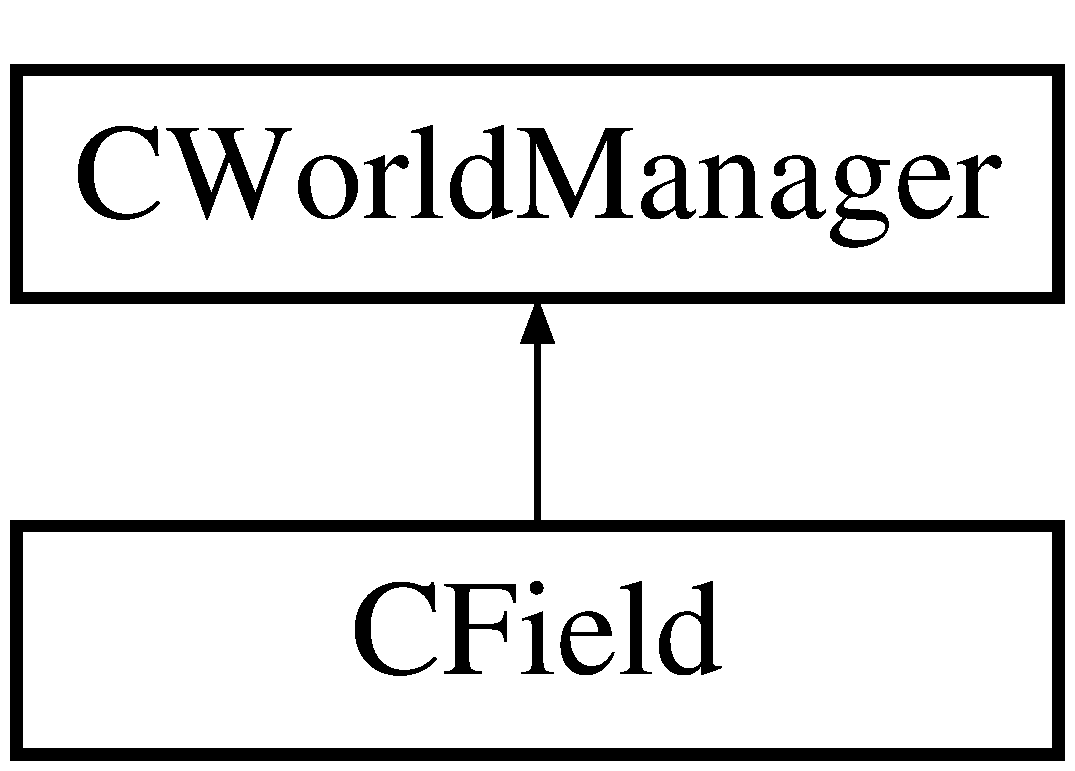
\includegraphics[height=2.000000cm]{class_c_field}
\end{center}
\end{figure}
\subsection*{Public Member Functions}
\begin{DoxyCompactItemize}
\item 
bool {\bfseries Init} (\hyperlink{structplaydata__tag}{playdata\+\_\+tag} $\ast$\+\_\+playdata\+\_\+p, const int \+\_\+dnum)\hypertarget{class_c_field_aeca01764ea3fa801e957396b0ec7ebe2}{}\label{class_c_field_aeca01764ea3fa801e957396b0ec7ebe2}

\item 
int {\bfseries Main\+Loop} ()\hypertarget{class_c_field_a7e7190d64b9b6ec0c8daef54edc6c21c}{}\label{class_c_field_a7e7190d64b9b6ec0c8daef54edc6c21c}

\item 
void \hyperlink{class_c_field_a7a9a8773b1277c3b9bb24695300e83f4}{Draw} (bool \+\_\+screenflip=false, bool \+\_\+textshowingstop=false, int dx=0, int dy=0, bool \+\_\+playeralsoshake=false)
\item 
bool {\bfseries Walk} (int \+\_\+dir, int \+\_\+walkspeed=0, bool \+\_\+eventwalk=false, bool \+\_\+walk=true, int \+\_\+fade=0)\hypertarget{class_c_field_a6bc0b60b618edb7542ada74214f43e79}{}\label{class_c_field_a6bc0b60b618edb7542ada74214f43e79}

\item 
void {\bfseries Jump} ()\hypertarget{class_c_field_a637d8d154c86aa3689e181740c783afb}{}\label{class_c_field_a637d8d154c86aa3689e181740c783afb}

\item 
int {\bfseries Get\+Now\+Map} ()\hypertarget{class_c_field_a4a8e2d4f4ab92bbc5c1a11447f2acfe6}{}\label{class_c_field_a4a8e2d4f4ab92bbc5c1a11447f2acfe6}

\item 
void {\bfseries Set\+Now\+Map} (int \+\_\+mapnum)\hypertarget{class_c_field_a26d1a70084c0c106749cc10c3a9b1e77}{}\label{class_c_field_a26d1a70084c0c106749cc10c3a9b1e77}

\item 
void {\bfseries Set\+Position} (int \+\_\+mapnum, int \+\_\+x, int \+\_\+y, bool \+\_\+d=false)\hypertarget{class_c_field_adbb9b4d407ed6d19c435a0096c6919e4}{}\label{class_c_field_adbb9b4d407ed6d19c435a0096c6919e4}

\item 
void {\bfseries Set\+My\+Pic} (const int \+\_\+img\mbox{[}C\+H\+A\+R\+A\+\_\+\+P\+I\+C\+\_\+\+N\+UM\mbox{]}, const char $\ast$\+\_\+pickey)\hypertarget{class_c_field_a59745375073813b2dabc0919eee79068}{}\label{class_c_field_a59745375073813b2dabc0919eee79068}

\item 
void {\bfseries Set\+My\+Dir} (int \+\_\+dir)\hypertarget{class_c_field_a94df6cb327cf2b049b99e03ed8820a1a}{}\label{class_c_field_a94df6cb327cf2b049b99e03ed8820a1a}

\item 
void {\bfseries Set\+My\+Visible} (bool \+\_\+visible)\hypertarget{class_c_field_ab34bc052be353dea0c928dd8adc7c957}{}\label{class_c_field_ab34bc052be353dea0c928dd8adc7c957}

\item 
void {\bfseries Set\+My\+Alpha} (unsigned char \+\_\+alpha)\hypertarget{class_c_field_ae02a68969dbd2520532253c14d9dd793}{}\label{class_c_field_ae02a68969dbd2520532253c14d9dd793}

\item 
void {\bfseries Set\+My\+Effect} (int \+\_\+effectname, int \+\_\+effectnum\mbox{[}$\,$\mbox{]})\hypertarget{class_c_field_a55706b18f51a664478f524bb36907d0a}{}\label{class_c_field_a55706b18f51a664478f524bb36907d0a}

\item 
void {\bfseries Set\+Game\+Mode} (gamemode\+\_\+tag \+\_\+mode)\hypertarget{class_c_field_ae07b7753fb0ae9413bf58be56fb723e7}{}\label{class_c_field_ae07b7753fb0ae9413bf58be56fb723e7}

\item 
gamemode\+\_\+tag {\bfseries Get\+Game\+Mode} ()\hypertarget{class_c_field_ab7835715d9a6e145d4d20cecb4beecaa}{}\label{class_c_field_ab7835715d9a6e145d4d20cecb4beecaa}

\item 
void {\bfseries Battle\+Start} (const char $\ast$\+\_\+pic\+\_\+bg, std\+::vector$<$ std\+::string $>$ \+\_\+enemy\+List)\hypertarget{class_c_field_aa9f2875d5175502c8d49a2455a462cb4}{}\label{class_c_field_aa9f2875d5175502c8d49a2455a462cb4}

\item 
void {\bfseries Battle\+Start} ()\hypertarget{class_c_field_aa22cd2ea834f50802329e3f4035c96d4}{}\label{class_c_field_aa22cd2ea834f50802329e3f4035c96d4}

\item 
void {\bfseries Set\+Battle\+Result} (const char $\ast$\+\_\+winmessage, const char $\ast$\+\_\+losemessage)\hypertarget{class_c_field_a0038d96053d468931a48ffe0f1447798}{}\label{class_c_field_a0038d96053d468931a48ffe0f1447798}

\item 
void {\bfseries Change\+Text\+Mode} (bool \+\_\+box, const char $\ast$\+\_\+eventtext=N\+U\+LL)\hypertarget{class_c_field_a1c495864a16b1546016e0e3c9abdeec8}{}\label{class_c_field_a1c495864a16b1546016e0e3c9abdeec8}

\end{DoxyCompactItemize}
\subsection*{Public Attributes}
\begin{DoxyCompactItemize}
\item 
\hyperlink{class_c_flag_set}{C\+Flag\+Set} {\bfseries Flag\+Set}\hypertarget{class_c_field_a90452af28b0f6497cfb40b88316a5d09}{}\label{class_c_field_a90452af28b0f6497cfb40b88316a5d09}

\end{DoxyCompactItemize}
\subsection*{Additional Inherited Members}


\subsection{Member Function Documentation}
\index{C\+Field@{C\+Field}!Draw@{Draw}}
\index{Draw@{Draw}!C\+Field@{C\+Field}}
\subsubsection[{\texorpdfstring{Draw(bool \+\_\+screenflip=false, bool \+\_\+textshowingstop=false, int dx=0, int dy=0, bool \+\_\+playeralsoshake=false)}{Draw(bool _screenflip=false, bool _textshowingstop=false, int dx=0, int dy=0, bool _playeralsoshake=false)}}]{\setlength{\rightskip}{0pt plus 5cm}void C\+Field\+::\+Draw (
\begin{DoxyParamCaption}
\item[{bool}]{\+\_\+screenflip = {\ttfamily false}, }
\item[{bool}]{\+\_\+textshowingstop = {\ttfamily false}, }
\item[{int}]{dx = {\ttfamily 0}, }
\item[{int}]{dy = {\ttfamily 0}, }
\item[{bool}]{\+\_\+playeralsoshake = {\ttfamily false}}
\end{DoxyParamCaption}
)\hspace{0.3cm}{\ttfamily [virtual]}}\hypertarget{class_c_field_a7a9a8773b1277c3b9bb24695300e83f4}{}\label{class_c_field_a7a9a8773b1277c3b9bb24695300e83f4}
神システム作りかけ//////////////////////////////////////////////////////////////// 

Implements \hyperlink{class_c_world_manager}{C\+World\+Manager}.



The documentation for this class was generated from the following files\+:\begin{DoxyCompactItemize}
\item 
Classes/Field.\+h\item 
Classes/Field.\+cpp\end{DoxyCompactItemize}

\hypertarget{class_c_field_cmd_manager}{}\section{C\+Field\+Cmd\+Manager Class Reference}
\label{class_c_field_cmd_manager}\index{C\+Field\+Cmd\+Manager@{C\+Field\+Cmd\+Manager}}
Inheritance diagram for C\+Field\+Cmd\+Manager\+:\begin{figure}[H]
\begin{center}
\leavevmode
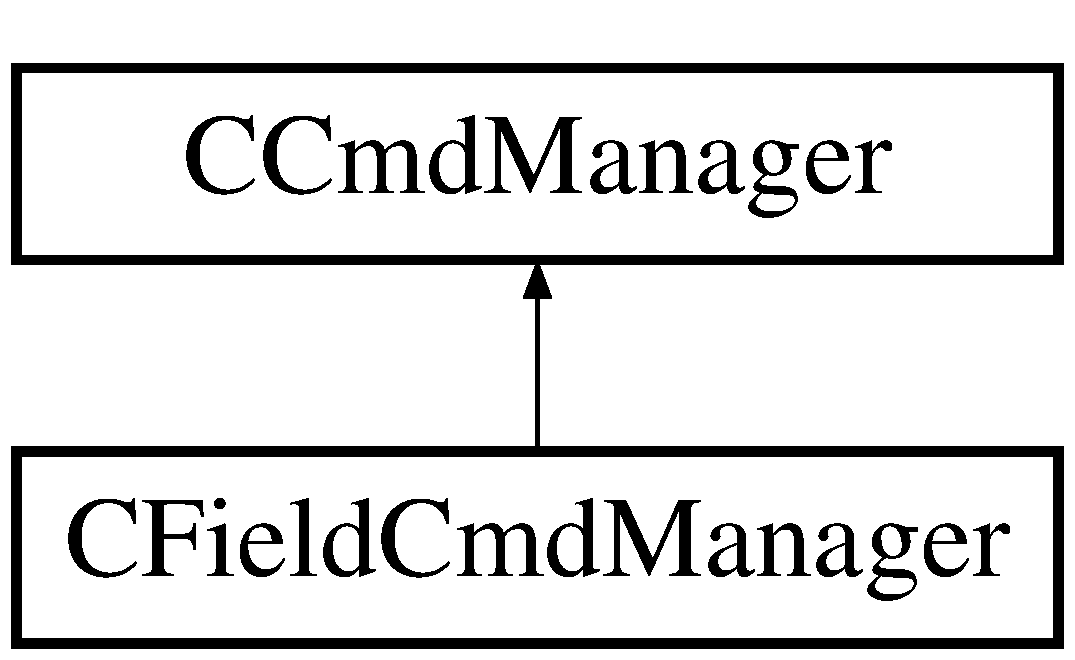
\includegraphics[height=2.000000cm]{class_c_field_cmd_manager}
\end{center}
\end{figure}
\subsection*{Public Member Functions}
\begin{DoxyCompactItemize}
\item 
void {\bfseries Main} (\hyperlink{class_c_cmd_list}{C\+Cmd\+List} $\ast$\+\_\+cmdlist, \hyperlink{class_c_field}{C\+Field} $\ast$\+\_\+field, \hyperlink{class_c_map}{C\+Map} $\ast$\+\_\+map, \hyperlink{class_c_text_box}{C\+Text\+Box} $\ast$\+\_\+textbox, \hyperlink{class_c_eve_manager}{C\+Eve\+Manager} $\ast$\+\_\+evemanager)\hypertarget{class_c_field_cmd_manager_afe22cb252b6d126fa8786145e2de6cd7}{}\label{class_c_field_cmd_manager_afe22cb252b6d126fa8786145e2de6cd7}

\end{DoxyCompactItemize}
\subsection*{Additional Inherited Members}


The documentation for this class was generated from the following files\+:\begin{DoxyCompactItemize}
\item 
Classes/Cmd\+Manager.\+h\item 
Classes/Cmd\+Manager.\+cpp\end{DoxyCompactItemize}

\hypertarget{class_c_field_log}{}\section{C\+Field\+Log Class Reference}
\label{class_c_field_log}\index{C\+Field\+Log@{C\+Field\+Log}}
Inheritance diagram for C\+Field\+Log\+:\begin{figure}[H]
\begin{center}
\leavevmode
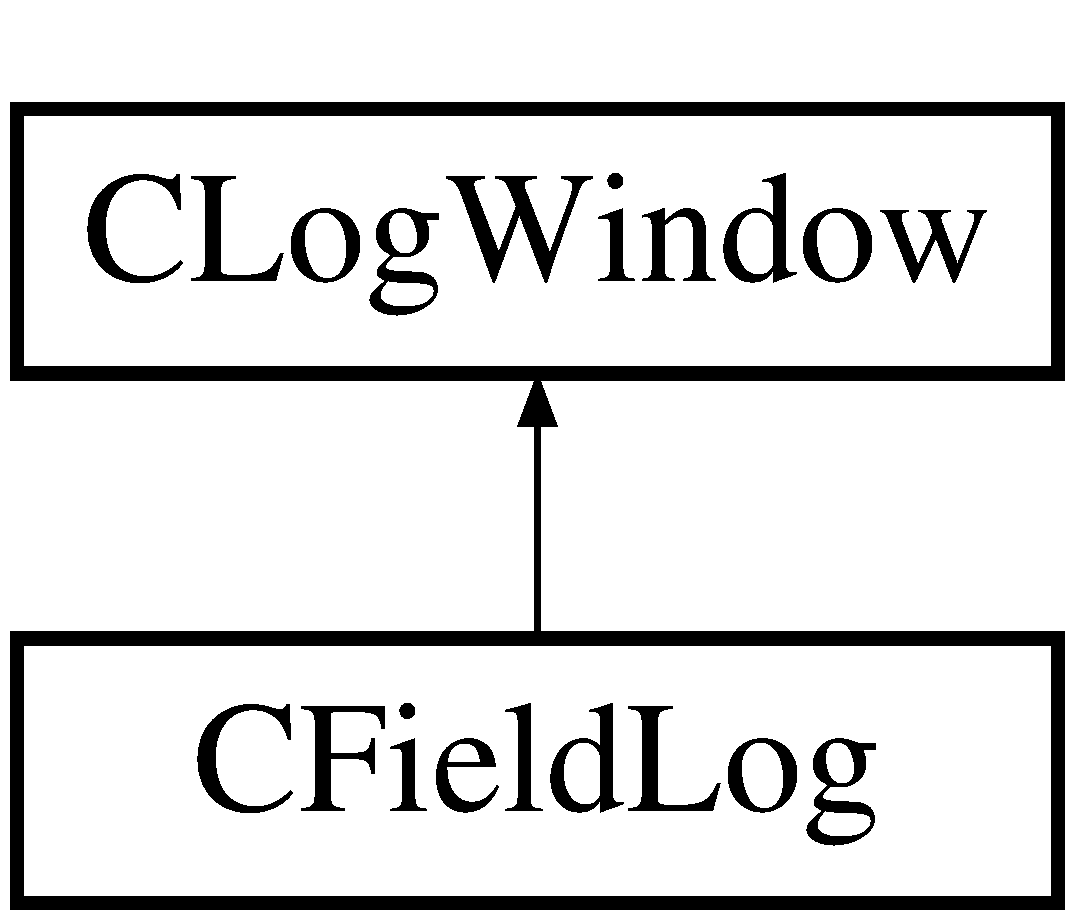
\includegraphics[height=2.000000cm]{class_c_field_log}
\end{center}
\end{figure}
\subsection*{Public Member Functions}
\begin{DoxyCompactItemize}
\item 
void {\bfseries Draw} ()\hypertarget{class_c_field_log_a9d5a6bc051de88cb011e92c61f71b1c8}{}\label{class_c_field_log_a9d5a6bc051de88cb011e92c61f71b1c8}

\item 
bool {\bfseries Main} ()\hypertarget{class_c_field_log_ab70929d9ae3f309979c464ffb51e63f9}{}\label{class_c_field_log_ab70929d9ae3f309979c464ffb51e63f9}

\item 
void {\bfseries Memorize\+Current\+Pos} ()\hypertarget{class_c_field_log_a977e85d9a3bf761bacca5f4a6a32fb16}{}\label{class_c_field_log_a977e85d9a3bf761bacca5f4a6a32fb16}

\item 
void {\bfseries Reset\+Current\+Pos} ()\hypertarget{class_c_field_log_a19044cb2e8de33f198668395fff44800}{}\label{class_c_field_log_a19044cb2e8de33f198668395fff44800}

\item 
void {\bfseries Insert\+To\+Memo\+Pos} (const char $\ast$\+\_\+string)\hypertarget{class_c_field_log_a3fb2407f1cefa14beab21e1af8ed2027}{}\label{class_c_field_log_a3fb2407f1cefa14beab21e1af8ed2027}

\end{DoxyCompactItemize}
\subsection*{Additional Inherited Members}


The documentation for this class was generated from the following files\+:\begin{DoxyCompactItemize}
\item 
Classes/Log\+Window.\+h\item 
Classes/Log\+Window.\+cpp\end{DoxyCompactItemize}

\hypertarget{class_c_field_menu}{}\section{C\+Field\+Menu Class Reference}
\label{class_c_field_menu}\index{C\+Field\+Menu@{C\+Field\+Menu}}
Inheritance diagram for C\+Field\+Menu\+:\begin{figure}[H]
\begin{center}
\leavevmode
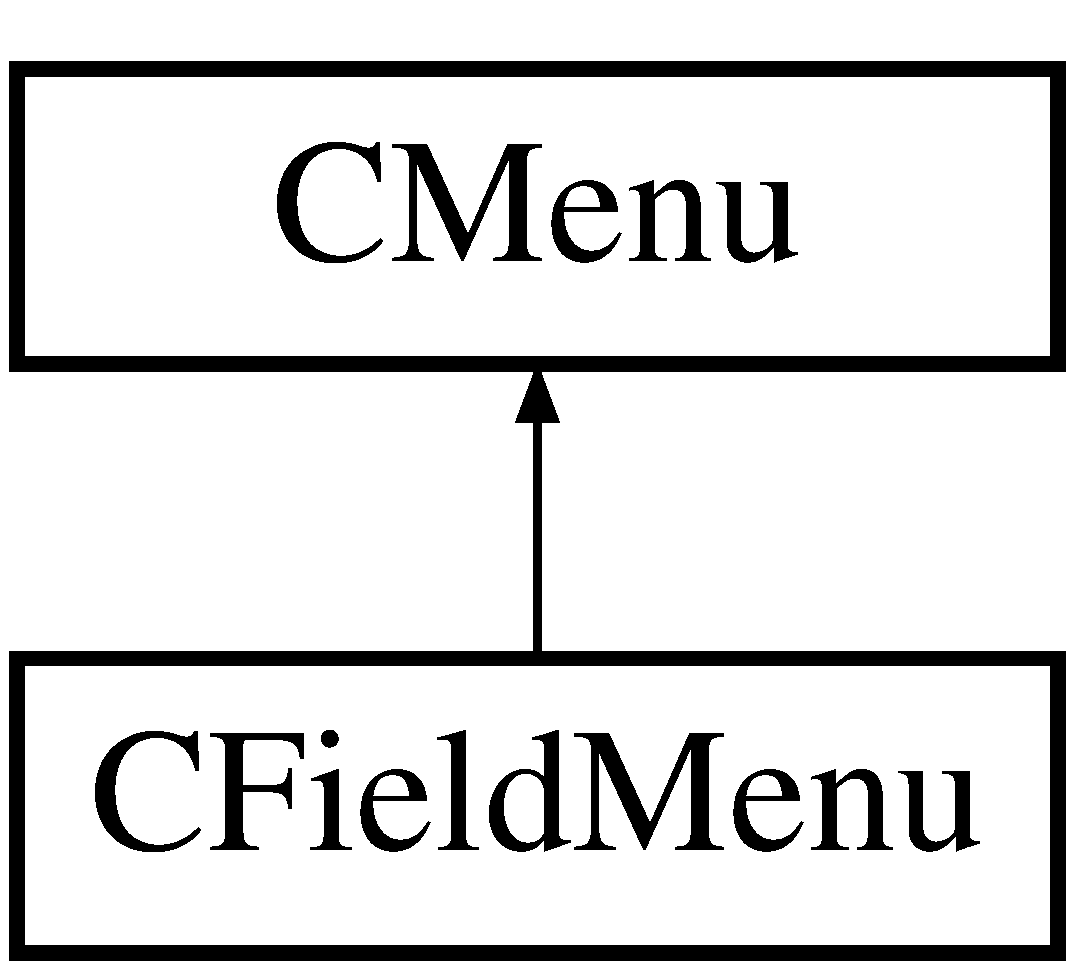
\includegraphics[height=2.000000cm]{class_c_field_menu}
\end{center}
\end{figure}
\subsection*{Public Member Functions}
\begin{DoxyCompactItemize}
\item 
void {\bfseries Draw} ()\hypertarget{class_c_field_menu_a5fce4cb692e50a7a0c691646a19c4cb3}{}\label{class_c_field_menu_a5fce4cb692e50a7a0c691646a19c4cb3}

\end{DoxyCompactItemize}
\subsection*{Public Attributes}
\begin{DoxyCompactItemize}
\item 
\hyperlink{class_c_menu}{C\+Menu} $\ast$ {\bfseries Accessory\+Menu}\hypertarget{class_c_field_menu_a70c71460e0ea554f36c8f2462d1c86cc}{}\label{class_c_field_menu_a70c71460e0ea554f36c8f2462d1c86cc}

\item 
bool {\bfseries Accessory\+Menu\+Visible}\hypertarget{class_c_field_menu_a99f77f502d132de4e20ed814ab9cc851}{}\label{class_c_field_menu_a99f77f502d132de4e20ed814ab9cc851}

\item 
int {\bfseries Accessory\+Slot\+Num}\hypertarget{class_c_field_menu_a9897ce6cf79c755a324d3495e8468fa7}{}\label{class_c_field_menu_a9897ce6cf79c755a324d3495e8468fa7}

\end{DoxyCompactItemize}
\subsection*{Additional Inherited Members}


The documentation for this class was generated from the following files\+:\begin{DoxyCompactItemize}
\item 
Classes/Menu.\+h\item 
Classes/Menu.\+cpp\end{DoxyCompactItemize}

\hypertarget{class_c_first_set_cmd_manager}{}\section{C\+First\+Set\+Cmd\+Manager Class Reference}
\label{class_c_first_set_cmd_manager}\index{C\+First\+Set\+Cmd\+Manager@{C\+First\+Set\+Cmd\+Manager}}
Inheritance diagram for C\+First\+Set\+Cmd\+Manager\+:\begin{figure}[H]
\begin{center}
\leavevmode
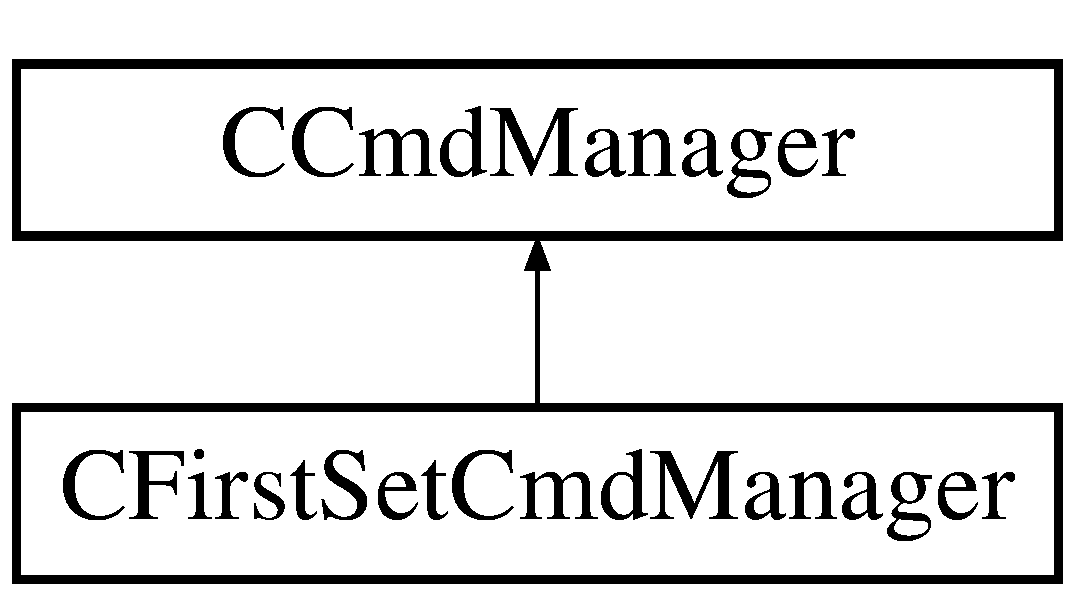
\includegraphics[height=2.000000cm]{class_c_first_set_cmd_manager}
\end{center}
\end{figure}
\subsection*{Public Member Functions}
\begin{DoxyCompactItemize}
\item 
void {\bfseries Main} (\hyperlink{class_c_cmd_list}{C\+Cmd\+List} $\ast$\+\_\+cmdlist, \hyperlink{class_c_field}{C\+Field} $\ast$\+\_\+field, \hyperlink{class_c_map}{C\+Map} $\ast$\+\_\+map, \hyperlink{class_c_eve_manager}{C\+Eve\+Manager} $\ast$\+\_\+evemanager)\hypertarget{class_c_first_set_cmd_manager_ae71edefdb48f39d6e7138158585f4cbc}{}\label{class_c_first_set_cmd_manager_ae71edefdb48f39d6e7138158585f4cbc}

\end{DoxyCompactItemize}
\subsection*{Additional Inherited Members}


The documentation for this class was generated from the following files\+:\begin{DoxyCompactItemize}
\item 
Classes/Cmd\+Manager.\+h\item 
Classes/Cmd\+Manager.\+cpp\end{DoxyCompactItemize}

\hypertarget{class_c_flag_set}{}\section{C\+Flag\+Set Class Reference}
\label{class_c_flag_set}\index{C\+Flag\+Set@{C\+Flag\+Set}}
\subsection*{Public Member Functions}
\begin{DoxyCompactItemize}
\item 
bool {\bfseries Create\+New\+Flag} (const char $\ast$\+\_\+key)\hypertarget{class_c_flag_set_a2195c9e21a9fafebe3088ee295f7abab}{}\label{class_c_flag_set_a2195c9e21a9fafebe3088ee295f7abab}

\item 
void {\bfseries Set\+Flag} (const char $\ast$\+\_\+key, int \+\_\+num=0, bool \+\_\+add=false, bool \+\_\+create=false)\hypertarget{class_c_flag_set_a599557b906f59a874eae13e6d21db76e}{}\label{class_c_flag_set_a599557b906f59a874eae13e6d21db76e}

\item 
int {\bfseries Get\+Flag\+Num} (const char $\ast$\+\_\+key)\hypertarget{class_c_flag_set_a618ab08a5941e5c3df9eaef7c9ac610d}{}\label{class_c_flag_set_a618ab08a5941e5c3df9eaef7c9ac610d}

\end{DoxyCompactItemize}
\subsection*{Public Attributes}
\begin{DoxyCompactItemize}
\item 
std\+::vector$<$ \hyperlink{structflag__tag}{flag\+\_\+tag} $>$ {\bfseries Flag}\hypertarget{class_c_flag_set_ad92fe96833f1bafb3919e579f5390cb1}{}\label{class_c_flag_set_ad92fe96833f1bafb3919e579f5390cb1}

\end{DoxyCompactItemize}


The documentation for this class was generated from the following file\+:\begin{DoxyCompactItemize}
\item 
Classes/Define.\+h\end{DoxyCompactItemize}

\hypertarget{structchar256}{}\section{char256 Struct Reference}
\label{structchar256}\index{char256@{char256}}
\subsection*{Public Member Functions}
\begin{DoxyCompactItemize}
\item 
bool {\bfseries operator$<$} (const \hyperlink{structchar256}{char256} \&obj) const \hypertarget{structchar256_ae1e38ad98d5f1cd7b21eb00f5379258e}{}\label{structchar256_ae1e38ad98d5f1cd7b21eb00f5379258e}

\item 
bool {\bfseries operator$>$} (const \hyperlink{structchar256}{char256} \&obj) const \hypertarget{structchar256_ac6ef98c7fbeb2792cfca198a7764b42a}{}\label{structchar256_ac6ef98c7fbeb2792cfca198a7764b42a}

\end{DoxyCompactItemize}
\subsection*{Public Attributes}
\begin{DoxyCompactItemize}
\item 
char {\bfseries text} \mbox{[}256\mbox{]}\hypertarget{structchar256_a86d4f7bb76a19f3b7eabeb4e8d86d472}{}\label{structchar256_a86d4f7bb76a19f3b7eabeb4e8d86d472}

\end{DoxyCompactItemize}


The documentation for this struct was generated from the following file\+:\begin{DoxyCompactItemize}
\item 
Classes/Define.\+h\end{DoxyCompactItemize}

\hypertarget{class_c_img_bank}{}\section{C\+Img\+Bank Class Reference}
\label{class_c_img_bank}\index{C\+Img\+Bank@{C\+Img\+Bank}}
Inheritance diagram for C\+Img\+Bank\+:\begin{figure}[H]
\begin{center}
\leavevmode
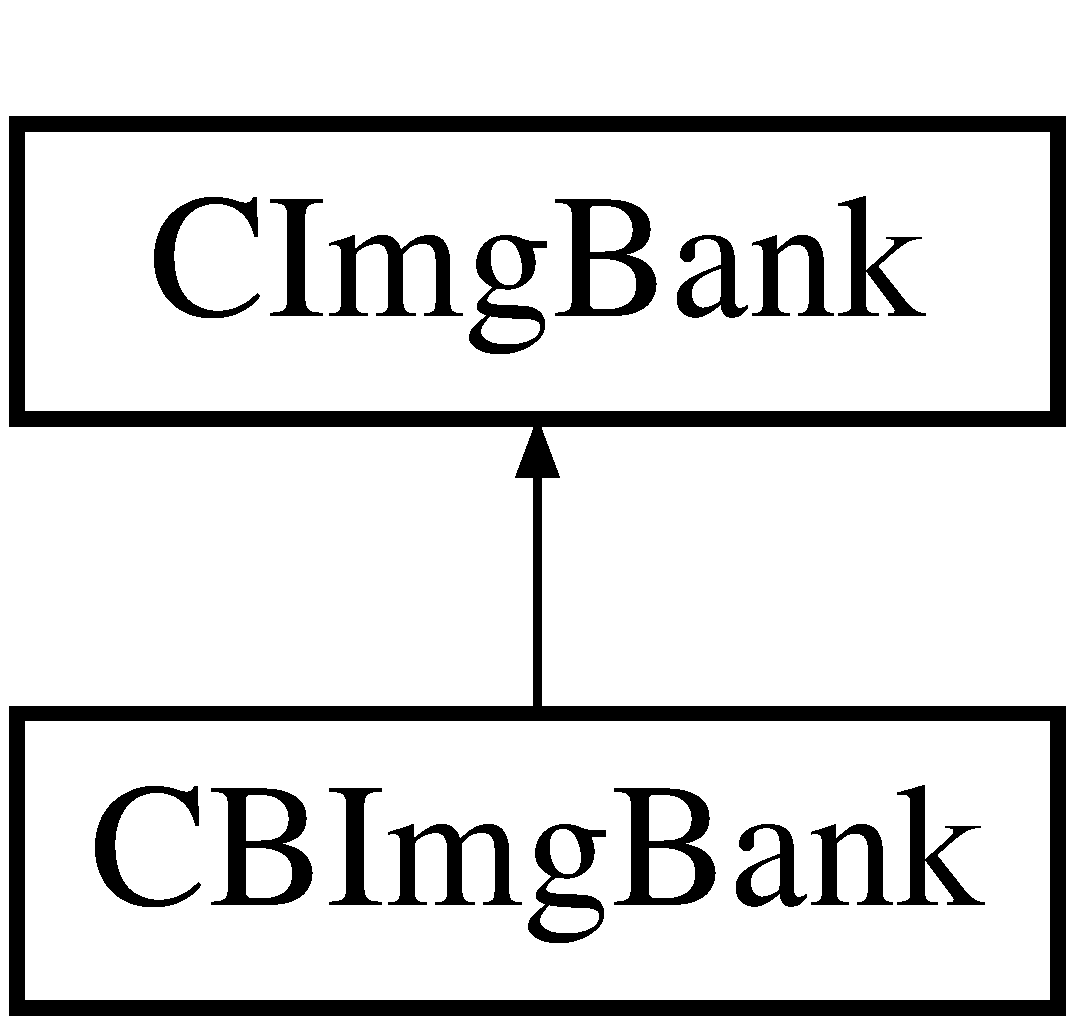
\includegraphics[height=2.000000cm]{class_c_img_bank}
\end{center}
\end{figure}
\subsection*{Public Member Functions}
\begin{DoxyCompactItemize}
\item 
void {\bfseries Clear} ()\hypertarget{class_c_img_bank_acbdbc031eaf2e16321bdb3218bd5c08a}{}\label{class_c_img_bank_acbdbc031eaf2e16321bdb3218bd5c08a}

\item 
void {\bfseries Load\+Pic} (const char $\ast$\+\_\+path, const char \+\_\+key\mbox{[}32\mbox{]}, const char \+\_\+kind\mbox{[}32\mbox{]})\hypertarget{class_c_img_bank_a827283e201d031f05f13cabdb438ae43}{}\label{class_c_img_bank_a827283e201d031f05f13cabdb438ae43}

\item 
bool {\bfseries Add\+Img} (const char $\ast$\+\_\+key, const int \+\_\+img, int \+\_\+sizeX=1, int \+\_\+sizeY=1)\hypertarget{class_c_img_bank_a48fd9cfdf57467cdae838856dc4dda17}{}\label{class_c_img_bank_a48fd9cfdf57467cdae838856dc4dda17}

\item 
int {\bfseries Get\+Img} (const char $\ast$\+\_\+key)\hypertarget{class_c_img_bank_aa22ec27911957938443c1a82a513f359}{}\label{class_c_img_bank_aa22ec27911957938443c1a82a513f359}

\item 
bool {\bfseries Get\+Img} (const char $\ast$\+\_\+key, int \+\_\+img\mbox{[}$\,$\mbox{]}, int \+\_\+sizeX, int \+\_\+sizeY=1)\hypertarget{class_c_img_bank_a507ac682ef4edf4294fe00100bf5f218}{}\label{class_c_img_bank_a507ac682ef4edf4294fe00100bf5f218}

\item 
int $\ast$ {\bfseries Get\+Img} (const char $\ast$\+\_\+key, int \+\_\+sizeX, int \+\_\+sizeY=1)\hypertarget{class_c_img_bank_a9297e7c5ab76a0a6bc7f89785db02ad3}{}\label{class_c_img_bank_a9297e7c5ab76a0a6bc7f89785db02ad3}

\end{DoxyCompactItemize}


The documentation for this class was generated from the following files\+:\begin{DoxyCompactItemize}
\item 
Classes/Img\+Bank.\+h\item 
Classes/Img\+Bank.\+cpp\end{DoxyCompactItemize}

\hypertarget{class_c_item}{}\section{C\+Item Class Reference}
\label{class_c_item}\index{C\+Item@{C\+Item}}
Inheritance diagram for C\+Item\+:\begin{figure}[H]
\begin{center}
\leavevmode
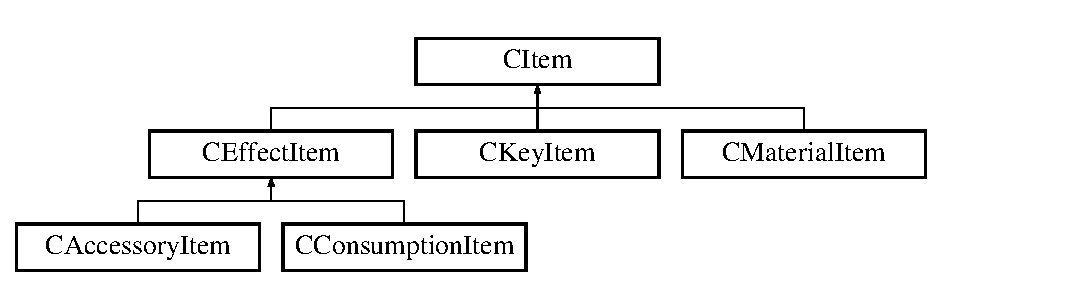
\includegraphics[height=3.000000cm]{class_c_item}
\end{center}
\end{figure}
\subsection*{Public Attributes}
\begin{DoxyCompactItemize}
\item 
std\+::string {\bfseries Name}\hypertarget{class_c_item_a1c72d0cdd2a18da3e8e80c7afdde828e}{}\label{class_c_item_a1c72d0cdd2a18da3e8e80c7afdde828e}

\item 
C\+Item\+Manager\+::item\+\_\+tag\+::type {\bfseries Kind}\hypertarget{class_c_item_afd15631a39190613aa14fdcc07a11d88}{}\label{class_c_item_afd15631a39190613aa14fdcc07a11d88}

\item 
int {\bfseries Own\+Limit}\hypertarget{class_c_item_a7d9cf16617730fac1065d0b33a329f09}{}\label{class_c_item_a7d9cf16617730fac1065d0b33a329f09}

\item 
int {\bfseries Price}\hypertarget{class_c_item_a48ac81e7d59d2f66ceb87f236791f98e}{}\label{class_c_item_a48ac81e7d59d2f66ceb87f236791f98e}

\item 
bool {\bfseries Sellable}\hypertarget{class_c_item_afb8ee5b88e34725d782ede5202d4c135}{}\label{class_c_item_afb8ee5b88e34725d782ede5202d4c135}

\end{DoxyCompactItemize}


The documentation for this class was generated from the following file\+:\begin{DoxyCompactItemize}
\item 
Classes/Item.\+h\end{DoxyCompactItemize}

\hypertarget{class_c_item_manager}{}\section{C\+Item\+Manager Class Reference}
\label{class_c_item_manager}\index{C\+Item\+Manager@{C\+Item\+Manager}}
\subsection*{Public Member Functions}
\begin{DoxyCompactItemize}
\item 
{\bfseries E\+N\+UM} (item\+\_\+tag, N\+O\+K\+I\+ND, C\+O\+N\+S\+U\+M\+P\+T\+I\+ON, A\+C\+C\+E\+S\+S\+O\+RY, K\+EY, M\+A\+T\+E\+R\+I\+AL)\hypertarget{class_c_item_manager_a5e95186104368015b674093bf9a4735a}{}\label{class_c_item_manager_a5e95186104368015b674093bf9a4735a}

\item 
void {\bfseries Init} ()\hypertarget{class_c_item_manager_a782a0f695d950a98f18d3e14ec1ac840}{}\label{class_c_item_manager_a782a0f695d950a98f18d3e14ec1ac840}

\item 
void {\bfseries Clear} ()\hypertarget{class_c_item_manager_aa20f0ea8d83f0c37395f2897b5b6a97f}{}\label{class_c_item_manager_aa20f0ea8d83f0c37395f2897b5b6a97f}

\item 
bool {\bfseries Add\+Item} (\hyperlink{class_c_item}{C\+Item} $\ast$\+\_\+new\+Item, const char $\ast$\+\_\+name, item\+\_\+tag\+::type \+\_\+kind, int \+\_\+own\+Limit, int \+\_\+price, bool \+\_\+sellable)\hypertarget{class_c_item_manager_ab09e43b1d2118f1f54a00307829df1e6}{}\label{class_c_item_manager_ab09e43b1d2118f1f54a00307829df1e6}

\item 
void {\bfseries Add\+Consumption\+Item} (const char $\ast$\+\_\+name, int \+\_\+own\+Limit, int \+\_\+price, bool \+\_\+sellable, bool \+\_\+battle\+Usable, int \+\_\+wait\+Time, target\+\_\+tag\+::type \+\_\+target, std\+::vector$<$ \hyperlink{structside_effect__tag}{side\+Effect\+\_\+tag} $>$ \+\_\+side\+Effect\+Set)\hypertarget{class_c_item_manager_a68c368c7cefc81227f317348dfbeeead}{}\label{class_c_item_manager_a68c368c7cefc81227f317348dfbeeead}

\item 
void {\bfseries Add\+Accessory\+Item} (const char $\ast$\+\_\+name, int \+\_\+own\+Limit, int \+\_\+price, bool \+\_\+sellable, std\+::vector$<$ std\+::pair$<$ std\+::string, int $>$ $>$ \+\_\+material\+Set, std\+::vector$<$ \hyperlink{structside_effect__tag}{side\+Effect\+\_\+tag} $>$ \+\_\+side\+Effect\+Set)\hypertarget{class_c_item_manager_a921bf797f85173d1a17828206b1d7773}{}\label{class_c_item_manager_a921bf797f85173d1a17828206b1d7773}

\item 
void {\bfseries Add\+Key\+Item} (const char $\ast$\+\_\+name, int \+\_\+own\+Limit, int \+\_\+price, bool \+\_\+sellable)\hypertarget{class_c_item_manager_a2d8ec3a84fb41ebe5fe72249ed549581}{}\label{class_c_item_manager_a2d8ec3a84fb41ebe5fe72249ed549581}

\item 
void {\bfseries Add\+Material\+Item} (const char $\ast$\+\_\+name, int \+\_\+own\+Limit, int \+\_\+price, bool \+\_\+sellable)\hypertarget{class_c_item_manager_a6df0255f5727ec0a5f024598f5d78ba0}{}\label{class_c_item_manager_a6df0255f5727ec0a5f024598f5d78ba0}

\item 
void {\bfseries Set\+Accessory\+Effect} (const char $\ast$\+\_\+name, std\+::vector$<$ \hyperlink{structside_effect__tag}{side\+Effect\+\_\+tag} $>$ \+\_\+side\+Effect\+Set)\hypertarget{class_c_item_manager_ae29aab01bdf60439343c654533ad1131}{}\label{class_c_item_manager_ae29aab01bdf60439343c654533ad1131}

\item 
\hyperlink{class_c_item}{C\+Item} $\ast$ {\bfseries Get\+Item} (std\+::string \+\_\+name)\hypertarget{class_c_item_manager_a2f9bef94df4a3bbf13d207a176876ced}{}\label{class_c_item_manager_a2f9bef94df4a3bbf13d207a176876ced}

\item 
\hyperlink{class_c_effect_item}{C\+Effect\+Item} $\ast$ {\bfseries Get\+Effect\+Item} (std\+::string \+\_\+name)\hypertarget{class_c_item_manager_a0bfb4dfcc31ef901102c8f1afeb98ff2}{}\label{class_c_item_manager_a0bfb4dfcc31ef901102c8f1afeb98ff2}

\item 
\hyperlink{class_c_consumption_item}{C\+Consumption\+Item} $\ast$ {\bfseries Get\+Consumption\+Item} (std\+::string \+\_\+name)\hypertarget{class_c_item_manager_ae1cd036f91edf392444c7c97013c4cfc}{}\label{class_c_item_manager_ae1cd036f91edf392444c7c97013c4cfc}

\item 
\hyperlink{class_c_accessory_item}{C\+Accessory\+Item} $\ast$ {\bfseries Get\+Accessory\+Item} (std\+::string \+\_\+name)\hypertarget{class_c_item_manager_a8959913f4df6eaf0048f1c02cd161f39}{}\label{class_c_item_manager_a8959913f4df6eaf0048f1c02cd161f39}

\item 
\hyperlink{class_c_menu}{C\+Menu} $\ast$ {\bfseries Get\+Player\+Accessory\+Menu} ()\hypertarget{class_c_item_manager_ac9a179e48bb8b18030c4fa0803a1cf86}{}\label{class_c_item_manager_ac9a179e48bb8b18030c4fa0803a1cf86}

\item 
bool {\bfseries Inc\+Player\+Item} (std\+::string \+\_\+name, int \+\_\+num)\hypertarget{class_c_item_manager_ae3f58e5d1dfcf85ebbc902128c8480ba}{}\label{class_c_item_manager_ae3f58e5d1dfcf85ebbc902128c8480ba}

\item 
bool {\bfseries Dec\+Player\+Item} (std\+::string \+\_\+name, int \+\_\+num)\hypertarget{class_c_item_manager_a9c1ba5359ffb008e6711b94d6696b1bd}{}\label{class_c_item_manager_a9c1ba5359ffb008e6711b94d6696b1bd}

\item 
int {\bfseries Get\+Player\+Item\+Num} (std\+::string \+\_\+name)\hypertarget{class_c_item_manager_affaa65031e648d9bc1a09c4258896618}{}\label{class_c_item_manager_affaa65031e648d9bc1a09c4258896618}

\item 
std\+::vector$<$ std\+::string $>$ {\bfseries Get\+Battle\+Item\+Name\+List} ()\hypertarget{class_c_item_manager_aa55d93d60045df5836e39df57866f842}{}\label{class_c_item_manager_aa55d93d60045df5836e39df57866f842}

\item 
std\+::vector$<$ std\+::string $>$ {\bfseries Get\+Accessory\+Item\+In\+Bag} ()\hypertarget{class_c_item_manager_a933fef668671a7145c52fbfe8b83561e}{}\label{class_c_item_manager_a933fef668671a7145c52fbfe8b83561e}

\item 
bool {\bfseries Inc\+Gold} (int \+\_\+gold)\hypertarget{class_c_item_manager_a9f21c82114045d9d47c63c7325f8cfc7}{}\label{class_c_item_manager_a9f21c82114045d9d47c63c7325f8cfc7}

\item 
bool {\bfseries Dec\+Gold} (int \+\_\+gold)\hypertarget{class_c_item_manager_a4b1ae73faf089194a4220263aea1e836}{}\label{class_c_item_manager_a4b1ae73faf089194a4220263aea1e836}

\item 
int {\bfseries Get\+Gold} ()\hypertarget{class_c_item_manager_aafa5c2e6278ff7d4af4bf603786af6c8}{}\label{class_c_item_manager_aafa5c2e6278ff7d4af4bf603786af6c8}

\item 
void {\bfseries Debug\+Show\+All\+Item} ()\hypertarget{class_c_item_manager_aea4544fbfc0ea5b040c52191416b6d79}{}\label{class_c_item_manager_aea4544fbfc0ea5b040c52191416b6d79}

\item 
void {\bfseries Debug\+Show\+All\+Player\+Item} ()\hypertarget{class_c_item_manager_a38fe8717821d31cde98f38932db474af}{}\label{class_c_item_manager_a38fe8717821d31cde98f38932db474af}

\end{DoxyCompactItemize}
\subsection*{Static Public Member Functions}
\begin{DoxyCompactItemize}
\item 
static \hyperlink{class_c_item_manager}{C\+Item\+Manager} $\ast$ {\bfseries Get\+Instance} ()\hypertarget{class_c_item_manager_a85451cfc18780bf97b932d3f22328afe}{}\label{class_c_item_manager_a85451cfc18780bf97b932d3f22328afe}

\end{DoxyCompactItemize}


The documentation for this class was generated from the following files\+:\begin{DoxyCompactItemize}
\item 
Classes/Item\+Manager.\+h\item 
Classes/Item\+Manager.\+cpp\end{DoxyCompactItemize}

\hypertarget{class_c_key_item}{}\section{C\+Key\+Item Class Reference}
\label{class_c_key_item}\index{C\+Key\+Item@{C\+Key\+Item}}
Inheritance diagram for C\+Key\+Item\+:\begin{figure}[H]
\begin{center}
\leavevmode
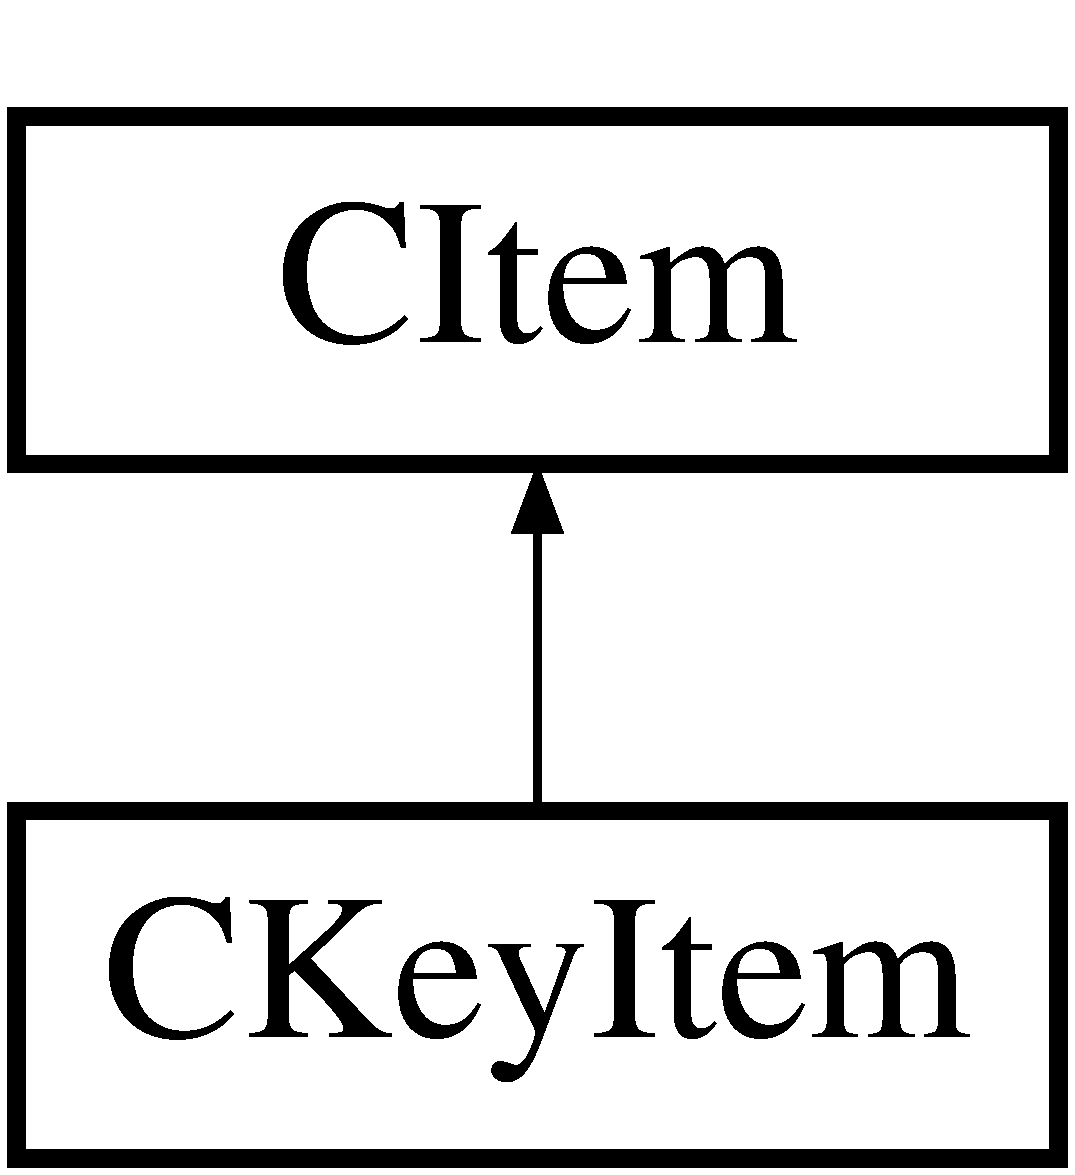
\includegraphics[height=2.000000cm]{class_c_key_item}
\end{center}
\end{figure}
\subsection*{Additional Inherited Members}


The documentation for this class was generated from the following file\+:\begin{DoxyCompactItemize}
\item 
Classes/Item.\+h\end{DoxyCompactItemize}

\hypertarget{classnunu_lib_key_1_1_c_key_manager}{}\section{nunu\+Lib\+Key\+:\+:C\+Key\+Manager Class Reference}
\label{classnunu_lib_key_1_1_c_key_manager}\index{nunu\+Lib\+Key\+::\+C\+Key\+Manager@{nunu\+Lib\+Key\+::\+C\+Key\+Manager}}
\subsection*{Public Member Functions}
\begin{DoxyCompactItemize}
\item 
bool {\bfseries Check\+Down} (const int K\+E\+Y\+\_\+\+C\+O\+DE)\hypertarget{classnunu_lib_key_1_1_c_key_manager_a5ea2d1b8c07df198fe98998af53a1d75}{}\label{classnunu_lib_key_1_1_c_key_manager_a5ea2d1b8c07df198fe98998af53a1d75}

\end{DoxyCompactItemize}


The documentation for this class was generated from the following files\+:\begin{DoxyCompactItemize}
\item 
Classes/nunu\+Lib.\+h\item 
Classes/nunu\+Lib.\+cpp\end{DoxyCompactItemize}

\hypertarget{class_c_load}{}\section{C\+Load Class Reference}
\label{class_c_load}\index{C\+Load@{C\+Load}}
\subsection*{Public Member Functions}
\begin{DoxyCompactItemize}
\item 
bool {\bfseries Load\+Add\+Text} (const char $\ast$\+\_\+path)\hypertarget{class_c_load_ad213efd3e154e1d5084795770f88db2b}{}\label{class_c_load_ad213efd3e154e1d5084795770f88db2b}

\item 
void {\bfseries Load\+Map} (const char $\ast$\+\_\+path, unsigned int \+\_\+mapnum, \hyperlink{class_c_map}{C\+Map} $\ast$\+\_\+map, \hyperlink{class_c_eve_manager}{C\+Eve\+Manager} $\ast$\+\_\+evemanager, bool \+\_\+event=false)\hypertarget{class_c_load_add5d5639d77f30edecda263bf32c608c}{}\label{class_c_load_add5d5639d77f30edecda263bf32c608c}

\item 
void {\bfseries Load\+Play\+Data} (\hyperlink{structplaydata__tag}{playdata\+\_\+tag} \+\_\+playdata\mbox{[}$\,$\mbox{]})\hypertarget{class_c_load_a101d280bf5246a3d9421c8b1f69bf1bf}{}\label{class_c_load_a101d280bf5246a3d9421c8b1f69bf1bf}

\item 
void {\bfseries Command\+Copy} (\hyperlink{class_c_cmd_list}{C\+Cmd\+List} $\ast$\+\_\+cmdlist)\hypertarget{class_c_load_a70838c218c15f8fa823beceece192a2d}{}\label{class_c_load_a70838c218c15f8fa823beceece192a2d}

\item 
void {\bfseries Event\+Text\+Copy} (\hyperlink{class_c_eve_manager}{C\+Eve\+Manager} $\ast$\+\_\+evemanager)\hypertarget{class_c_load_ae92a2bfb056d9aca923122abafd06858}{}\label{class_c_load_ae92a2bfb056d9aca923122abafd06858}

\end{DoxyCompactItemize}


The documentation for this class was generated from the following files\+:\begin{DoxyCompactItemize}
\item 
Classes/Load.\+h\item 
Classes/Load.\+cpp\end{DoxyCompactItemize}

\hypertarget{class_c_log_window}{}\section{C\+Log\+Window Class Reference}
\label{class_c_log_window}\index{C\+Log\+Window@{C\+Log\+Window}}
Inheritance diagram for C\+Log\+Window\+:\begin{figure}[H]
\begin{center}
\leavevmode
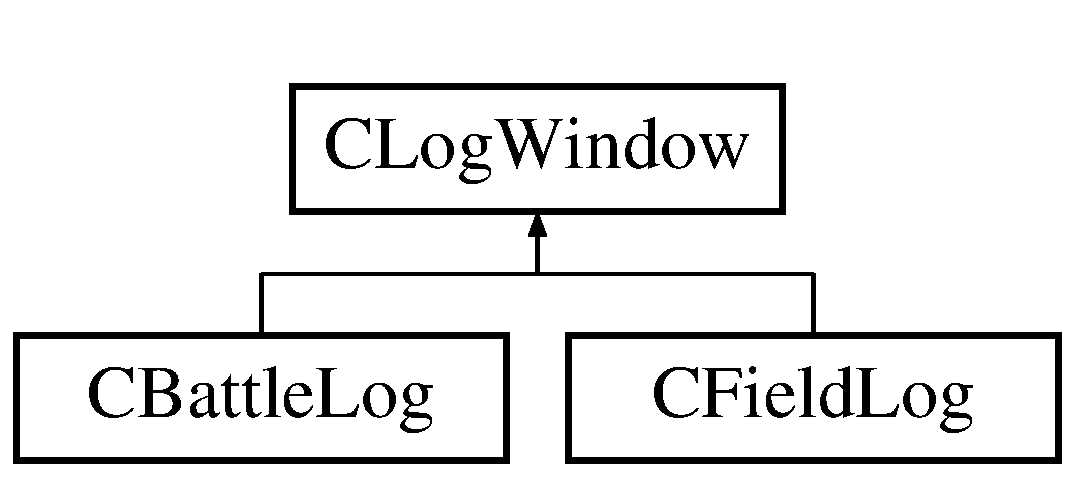
\includegraphics[height=2.000000cm]{class_c_log_window}
\end{center}
\end{figure}
\subsection*{Public Member Functions}
\begin{DoxyCompactItemize}
\item 
virtual void {\bfseries Init} (int \+\_\+posx, int \+\_\+posy, int \+\_\+width, int \+\_\+height, int \+\_\+box\+Color, int \+\_\+stock\+Line, int \+\_\+font\+Size, int \+\_\+font\+Color\+Main, int \+\_\+font\+Color\+Sub)\hypertarget{class_c_log_window_a0b6d6ccdd24a98ab6e3f8e81e8ce657f}{}\label{class_c_log_window_a0b6d6ccdd24a98ab6e3f8e81e8ce657f}

\item 
void {\bfseries Clear} ()\hypertarget{class_c_log_window_ae01f51f5e163ba75699fa939ad0a8671}{}\label{class_c_log_window_ae01f51f5e163ba75699fa939ad0a8671}

\item 
void {\bfseries Term} ()\hypertarget{class_c_log_window_a17c0b89a15894edd9e6d919a3905ea60}{}\label{class_c_log_window_a17c0b89a15894edd9e6d919a3905ea60}

\item 
bool {\bfseries Add} (const char $\ast$\+\_\+format,...)\hypertarget{class_c_log_window_afc806191594ec4c93ac347a27d7e21c2}{}\label{class_c_log_window_afc806191594ec4c93ac347a27d7e21c2}

\item 
bool {\bfseries Add} (char $\ast$$\ast$\+\_\+new\+Text\+Array)\hypertarget{class_c_log_window_a5f8775f3bd9c29b381c97ac56c11380c}{}\label{class_c_log_window_a5f8775f3bd9c29b381c97ac56c11380c}

\item 
bool {\bfseries Main} ()\hypertarget{class_c_log_window_acb4cc76ab066eb3b6c681d3f540b36ba}{}\label{class_c_log_window_acb4cc76ab066eb3b6c681d3f540b36ba}

\item 
void {\bfseries Set\+Visible} (bool \+\_\+visible)\hypertarget{class_c_log_window_a4bb269245a2cfdfe05b2e4fdc7e9822d}{}\label{class_c_log_window_a4bb269245a2cfdfe05b2e4fdc7e9822d}

\end{DoxyCompactItemize}
\subsection*{Protected Types}
\begin{DoxyCompactItemize}
\item 
enum \{ {\bfseries W\+O\+R\+D\+\_\+\+M\+AX} = 255
 \}\hypertarget{class_c_log_window_ab5fed1a6f695003cf6bfae4f4c45b55d}{}\label{class_c_log_window_ab5fed1a6f695003cf6bfae4f4c45b55d}

\end{DoxyCompactItemize}
\subsection*{Protected Attributes}
\begin{DoxyCompactItemize}
\item 
bool {\bfseries Initialized}\hypertarget{class_c_log_window_a986a16a267c2d41363fe066314de4ee0}{}\label{class_c_log_window_a986a16a267c2d41363fe066314de4ee0}

\item 
char $\ast$$\ast$ {\bfseries Text}\hypertarget{class_c_log_window_a5c2399c56c2d02ee61ed9b733eaa6e27}{}\label{class_c_log_window_a5c2399c56c2d02ee61ed9b733eaa6e27}

\item 
int {\bfseries PosX}\hypertarget{class_c_log_window_a488d5b3a21d0f2d9e645c927fe0d9193}{}\label{class_c_log_window_a488d5b3a21d0f2d9e645c927fe0d9193}

\item 
int {\bfseries PosY}\hypertarget{class_c_log_window_ada10328613c4c8d2c9951927d9ba9607}{}\label{class_c_log_window_ada10328613c4c8d2c9951927d9ba9607}

\item 
int {\bfseries Width}\hypertarget{class_c_log_window_a94a87aabd208f92d49ab18597481f9f6}{}\label{class_c_log_window_a94a87aabd208f92d49ab18597481f9f6}

\item 
int {\bfseries Height}\hypertarget{class_c_log_window_afc77264b35d52aca76b03d1781721ddc}{}\label{class_c_log_window_afc77264b35d52aca76b03d1781721ddc}

\item 
int {\bfseries Stock\+Line\+Num}\hypertarget{class_c_log_window_a8d02ef592034112a45318e834bcfde28}{}\label{class_c_log_window_a8d02ef592034112a45318e834bcfde28}

\item 
int {\bfseries Line\+Num}\hypertarget{class_c_log_window_a79881c437c121f840d17b33cbf7f105c}{}\label{class_c_log_window_a79881c437c121f840d17b33cbf7f105c}

\item 
int {\bfseries Word\+Num}\hypertarget{class_c_log_window_a0faa55b1a0e06369a7dc36bc34898632}{}\label{class_c_log_window_a0faa55b1a0e06369a7dc36bc34898632}

\item 
int {\bfseries Line\+Space}\hypertarget{class_c_log_window_a878cbc283249a725d9f437e0c5787865}{}\label{class_c_log_window_a878cbc283249a725d9f437e0c5787865}

\item 
int {\bfseries Box\+Space}\hypertarget{class_c_log_window_a71c20095ebb24561e84b3e1c5389b74f}{}\label{class_c_log_window_a71c20095ebb24561e84b3e1c5389b74f}

\item 
int {\bfseries Font\+Size}\hypertarget{class_c_log_window_a747cd3ed8bdf5c7e6330ada3d4c6d5bf}{}\label{class_c_log_window_a747cd3ed8bdf5c7e6330ada3d4c6d5bf}

\item 
int {\bfseries Font\+Handle}\hypertarget{class_c_log_window_a5ae2447c2563b8a46da2225f45a7276d}{}\label{class_c_log_window_a5ae2447c2563b8a46da2225f45a7276d}

\item 
int {\bfseries Font\+Color\+Main}\hypertarget{class_c_log_window_a18b4391f11e86c99c4e0ae0e3e4c2394}{}\label{class_c_log_window_a18b4391f11e86c99c4e0ae0e3e4c2394}

\item 
int {\bfseries Font\+Color\+Sub}\hypertarget{class_c_log_window_a940601d6766f58c69f098b4c3a65978d}{}\label{class_c_log_window_a940601d6766f58c69f098b4c3a65978d}

\item 
int {\bfseries Box\+Color}\hypertarget{class_c_log_window_a3d122cd2b94fce6a7605d9b939ae47ca}{}\label{class_c_log_window_a3d122cd2b94fce6a7605d9b939ae47ca}

\item 
int {\bfseries Word\+Width}\hypertarget{class_c_log_window_aaf8a0fe5375d196e74b0e248e924c6a6}{}\label{class_c_log_window_aaf8a0fe5375d196e74b0e248e924c6a6}

\item 
int {\bfseries Next\+Line}\hypertarget{class_c_log_window_a33e2679a3f3c571d98860157f325bbda}{}\label{class_c_log_window_a33e2679a3f3c571d98860157f325bbda}

\item 
int {\bfseries Back\+Line}\hypertarget{class_c_log_window_a52511a0c99cac64c2d9097d8fad00937}{}\label{class_c_log_window_a52511a0c99cac64c2d9097d8fad00937}

\item 
bool {\bfseries Visible}\hypertarget{class_c_log_window_afee3508c4ea142dde092560d579c5688}{}\label{class_c_log_window_afee3508c4ea142dde092560d579c5688}

\end{DoxyCompactItemize}


The documentation for this class was generated from the following files\+:\begin{DoxyCompactItemize}
\item 
Classes/Log\+Window.\+h\item 
Classes/Log\+Window.\+cpp\end{DoxyCompactItemize}

\hypertarget{class_c_main}{}\section{C\+Main Class Reference}
\label{class_c_main}\index{C\+Main@{C\+Main}}
\subsection*{Public Member Functions}
\begin{DoxyCompactItemize}
\item 
bool {\bfseries Init} ()\hypertarget{class_c_main_a4670e6ec18a9d37e7c4eaa434fd05960}{}\label{class_c_main_a4670e6ec18a9d37e7c4eaa434fd05960}

\item 
bool {\bfseries Game\+Loop} ()\hypertarget{class_c_main_a78bb32c2155fb61d5f7c137b3134cdfb}{}\label{class_c_main_a78bb32c2155fb61d5f7c137b3134cdfb}

\end{DoxyCompactItemize}
\subsection*{Static Public Member Functions}
\begin{DoxyCompactItemize}
\item 
static \hyperlink{class_c_main}{C\+Main} $\ast$ {\bfseries Get\+Instance} ()\hypertarget{class_c_main_a75cc0f5be6ff981a22b094fedb091804}{}\label{class_c_main_a75cc0f5be6ff981a22b094fedb091804}

\end{DoxyCompactItemize}


The documentation for this class was generated from the following files\+:\begin{DoxyCompactItemize}
\item 
Classes/Main.\+h\item 
Classes/Main.\+cpp\end{DoxyCompactItemize}

\hypertarget{class_c_map}{}\section{C\+Map Class Reference}
\label{class_c_map}\index{C\+Map@{C\+Map}}
\subsection*{Public Member Functions}
\begin{DoxyCompactItemize}
\item 
void {\bfseries Init} ()\hypertarget{class_c_map_a604f597cf8d0f5a5428bceba203f8550}{}\label{class_c_map_a604f597cf8d0f5a5428bceba203f8550}

\item 
void {\bfseries Draw} (int \+\_\+mapnum, int \+\_\+x, int \+\_\+y, int \+\_\+dx=0, int \+\_\+dy=0)\hypertarget{class_c_map_a697a1a7f8c1b05f7d8b54117500ef5de}{}\label{class_c_map_a697a1a7f8c1b05f7d8b54117500ef5de}

\item 
void {\bfseries Set\+Map} (unsigned int \+\_\+mapnum, int \+\_\+filesize, unsigned char $\ast$buf)\hypertarget{class_c_map_aa87f821718e8b827d3f1d4cda73defb8}{}\label{class_c_map_aa87f821718e8b827d3f1d4cda73defb8}

\item 
void {\bfseries Load\+Chip} (const char $\ast$\+\_\+path, int \+\_\+mapnum, bool \+\_\+mapchip=true)\hypertarget{class_c_map_a8eb9c47a12b45ae2b55219d7f8884ee7}{}\label{class_c_map_a8eb9c47a12b45ae2b55219d7f8884ee7}

\item 
void {\bfseries Load\+Pic} (const char $\ast$\+\_\+path, const char \+\_\+key\mbox{[}32\mbox{]}, const char \+\_\+kind\mbox{[}32\mbox{]}=N\+U\+LL)\hypertarget{class_c_map_a02f624d8b14ecf59fe871872262e7e77}{}\label{class_c_map_a02f624d8b14ecf59fe871872262e7e77}

\item 
void {\bfseries Create\+Map\+Graph} (int \+\_\+mapnum=-\/1)\hypertarget{class_c_map_a68f7a6f87f0329e8240f6cb80cc8066d}{}\label{class_c_map_a68f7a6f87f0329e8240f6cb80cc8066d}

\item 
int {\bfseries Get\+Map\+Data} (int \+\_\+mapnum, int \+\_\+x, int \+\_\+y, int layer=0)\hypertarget{class_c_map_a40d05db9c083b83ad7f950b79924641e}{}\label{class_c_map_a40d05db9c083b83ad7f950b79924641e}

\item 
int $\ast$ {\bfseries Get\+Img\+Data} (const char \+\_\+key\mbox{[}32\mbox{]})\hypertarget{class_c_map_a326beaf995b046a34a6a36cc2a260f97}{}\label{class_c_map_a326beaf995b046a34a6a36cc2a260f97}

\item 
bool {\bfseries Set\+Map\+Music} (int \+\_\+map\+Num, std\+::string \+\_\+music\+Key, bool \+\_\+is\+Battle=false)\hypertarget{class_c_map_aaa9849b77dc02cee31077c9c8b5a95f6}{}\label{class_c_map_aaa9849b77dc02cee31077c9c8b5a95f6}

\item 
std\+::string {\bfseries Get\+Map\+Music} (int \+\_\+map\+Num, bool \+\_\+is\+Battle=false)\hypertarget{class_c_map_ac0010b80157b3bcc5e4b71949208e5a3}{}\label{class_c_map_ac0010b80157b3bcc5e4b71949208e5a3}

\end{DoxyCompactItemize}


The documentation for this class was generated from the following files\+:\begin{DoxyCompactItemize}
\item 
Classes/Map.\+h\item 
Classes/Map.\+cpp\end{DoxyCompactItemize}

\hypertarget{class_c_material_item}{}\section{C\+Material\+Item Class Reference}
\label{class_c_material_item}\index{C\+Material\+Item@{C\+Material\+Item}}
Inheritance diagram for C\+Material\+Item\+:\begin{figure}[H]
\begin{center}
\leavevmode
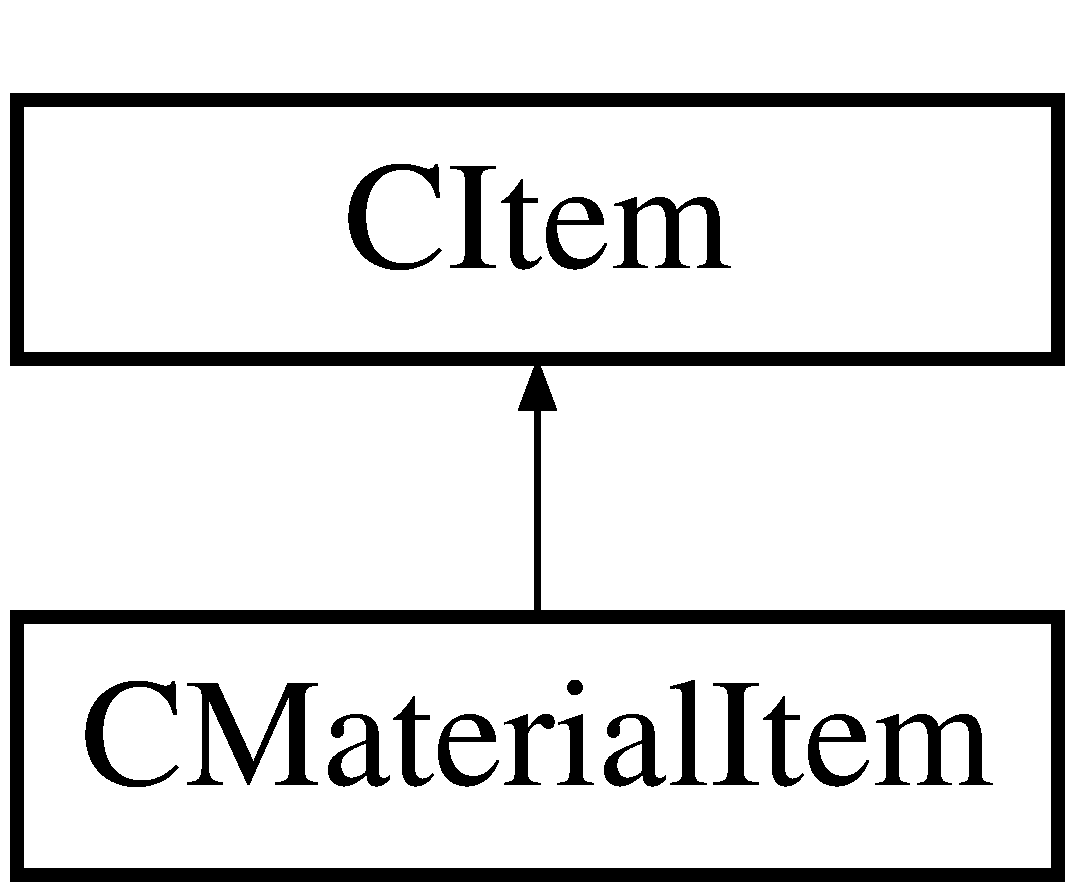
\includegraphics[height=2.000000cm]{class_c_material_item}
\end{center}
\end{figure}
\subsection*{Additional Inherited Members}


The documentation for this class was generated from the following file\+:\begin{DoxyCompactItemize}
\item 
Classes/Item.\+h\end{DoxyCompactItemize}

\hypertarget{class_c_menu}{}\section{C\+Menu Class Reference}
\label{class_c_menu}\index{C\+Menu@{C\+Menu}}
Inheritance diagram for C\+Menu\+:\begin{figure}[H]
\begin{center}
\leavevmode
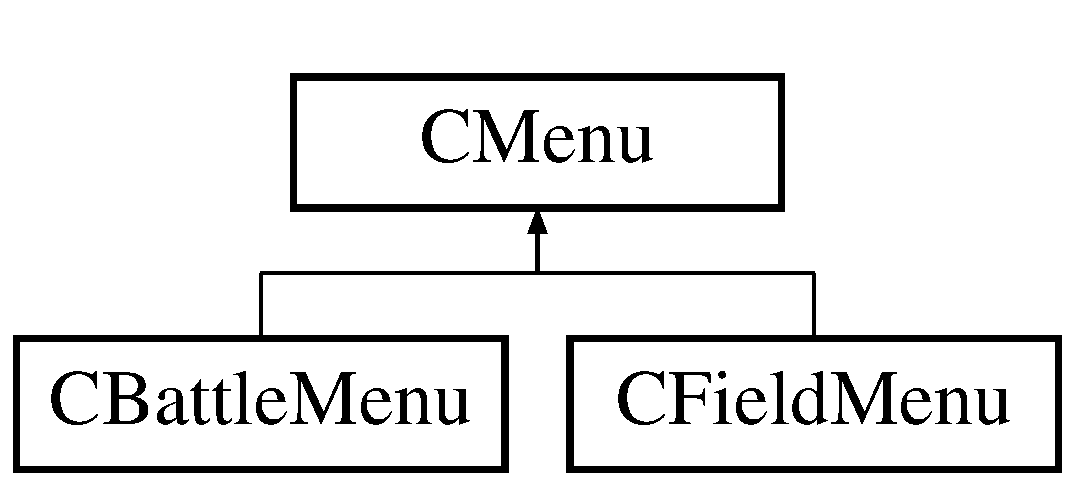
\includegraphics[height=2.000000cm]{class_c_menu}
\end{center}
\end{figure}
\subsection*{Public Member Functions}
\begin{DoxyCompactItemize}
\item 
void {\bfseries Clear} ()\hypertarget{class_c_menu_a0d6d9a0ed33c1865fe0ff937c2ad975f}{}\label{class_c_menu_a0d6d9a0ed33c1865fe0ff937c2ad975f}

\item 
void {\bfseries Init} (int \+\_\+x, int \+\_\+y, int \+\_\+width, int \+\_\+height)\hypertarget{class_c_menu_aedb6253ad2edea03b71011142d5f6f49}{}\label{class_c_menu_aedb6253ad2edea03b71011142d5f6f49}

\item 
void {\bfseries Create} (\hyperlink{class_c_menu_node}{C\+Menu\+Node} $\ast$\+\_\+group\+Parent)\hypertarget{class_c_menu_a4d792978b708a1cf09e83b2ce2e31786}{}\label{class_c_menu_a4d792978b708a1cf09e83b2ce2e31786}

\item 
void {\bfseries Create} (const char \+\_\+frontlabel\mbox{[}32\mbox{]})\hypertarget{class_c_menu_a06a10a9122f369cd57f502a6f38d3f55}{}\label{class_c_menu_a06a10a9122f369cd57f502a6f38d3f55}

\item 
void {\bfseries Add} (const char \+\_\+parentlabel\mbox{[}32\mbox{]}, \hyperlink{class_c_menu_node}{C\+Menu\+Node} $\ast$\+\_\+group\+Parent)\hypertarget{class_c_menu_ae9fef7c97d7de8f11c7f6a6a0dffaad8}{}\label{class_c_menu_ae9fef7c97d7de8f11c7f6a6a0dffaad8}

\item 
void {\bfseries Add} (const char \+\_\+parentlabel\mbox{[}32\mbox{]}, const char \+\_\+newlabel\mbox{[}32\mbox{]})\hypertarget{class_c_menu_ac6a2b27353ac1abac1cc6d15c210e0c8}{}\label{class_c_menu_ac6a2b27353ac1abac1cc6d15c210e0c8}

\item 
void {\bfseries Set\+Cursor} (\hyperlink{class_c_menu_node}{C\+Menu\+Node} $\ast$\+\_\+node)\hypertarget{class_c_menu_adaf997921c71f28726a990d36873a2d8}{}\label{class_c_menu_adaf997921c71f28726a990d36873a2d8}

\item 
\hyperlink{class_c_menu_node}{C\+Menu\+Node} $\ast$ {\bfseries Get\+Cursor} ()\hypertarget{class_c_menu_ab67f44905e3e4d296c3a47c1e32b49bd}{}\label{class_c_menu_ab67f44905e3e4d296c3a47c1e32b49bd}

\item 
\hyperlink{class_c_menu_node}{C\+Menu\+Node} $\ast$ {\bfseries Get\+Front} ()\hypertarget{class_c_menu_a8ebb7822ccfd66c7dcbcce2781499fba}{}\label{class_c_menu_a8ebb7822ccfd66c7dcbcce2781499fba}

\item 
\hyperlink{class_c_menu_node}{C\+Menu\+Node} $\ast$ {\bfseries Find} (const char \+\_\+label\mbox{[}32\mbox{]})\hypertarget{class_c_menu_a7df4a60ce0c2654f92c770c500f33576}{}\label{class_c_menu_a7df4a60ce0c2654f92c770c500f33576}

\item 
int {\bfseries Get\+Index} (\hyperlink{class_c_menu_node}{C\+Menu\+Node} $\ast$\+\_\+node)\hypertarget{class_c_menu_a4eae259ca5876075f4502a7138e22de0}{}\label{class_c_menu_a4eae259ca5876075f4502a7138e22de0}

\item 
bool {\bfseries Move} (\hyperlink{class_c_menu_node}{C\+Menu\+Node} $\ast$\&\+\_\+result, bool \+\_\+at\+Tip)\hypertarget{class_c_menu_a54d76f69aeb7b5c24213f294538b85a7}{}\label{class_c_menu_a54d76f69aeb7b5c24213f294538b85a7}

\end{DoxyCompactItemize}
\subsection*{Public Attributes}
\begin{DoxyCompactItemize}
\item 
bool {\bfseries Alive}\hypertarget{class_c_menu_a8ee14e0a0d7bdddd70a60388d1535578}{}\label{class_c_menu_a8ee14e0a0d7bdddd70a60388d1535578}

\end{DoxyCompactItemize}
\subsection*{Protected Attributes}
\begin{DoxyCompactItemize}
\item 
int {\bfseries X}\hypertarget{class_c_menu_ac8a6e07179118de0d2d0559c818fde01}{}\label{class_c_menu_ac8a6e07179118de0d2d0559c818fde01}

\item 
int {\bfseries Y}\hypertarget{class_c_menu_aa21585a21f674ffe6b74c11769784248}{}\label{class_c_menu_aa21585a21f674ffe6b74c11769784248}

\item 
int {\bfseries Width}\hypertarget{class_c_menu_a46e5a8e40fdeb225658b306481345684}{}\label{class_c_menu_a46e5a8e40fdeb225658b306481345684}

\item 
int {\bfseries Height}\hypertarget{class_c_menu_ab23bc5592efa0860e90ac60b8c115a38}{}\label{class_c_menu_ab23bc5592efa0860e90ac60b8c115a38}

\item 
\hyperlink{class_c_menu_node}{C\+Menu\+Node} $\ast$ {\bfseries Cursor}\hypertarget{class_c_menu_a6bd7b1f8e6838465c15d1985986f29fe}{}\label{class_c_menu_a6bd7b1f8e6838465c15d1985986f29fe}

\end{DoxyCompactItemize}


The documentation for this class was generated from the following files\+:\begin{DoxyCompactItemize}
\item 
Classes/Menu.\+h\item 
Classes/Menu.\+cpp\end{DoxyCompactItemize}

\hypertarget{class_c_menu_node}{}\section{C\+Menu\+Node Class Reference}
\label{class_c_menu_node}\index{C\+Menu\+Node@{C\+Menu\+Node}}
\subsection*{Public Member Functions}
\begin{DoxyCompactItemize}
\item 
{\bfseries C\+Menu\+Node} (const char \+\_\+label\mbox{[}32\mbox{]})\hypertarget{class_c_menu_node_ab649e9df54411fc974a57ea15ad48067}{}\label{class_c_menu_node_ab649e9df54411fc974a57ea15ad48067}

\end{DoxyCompactItemize}
\subsection*{Public Attributes}
\begin{DoxyCompactItemize}
\item 
char {\bfseries label} \mbox{[}32\mbox{]}\hypertarget{class_c_menu_node_a83e10a281e2c0af53452506eff9c78c1}{}\label{class_c_menu_node_a83e10a281e2c0af53452506eff9c78c1}

\item 
\hyperlink{class_c_menu_node}{C\+Menu\+Node} $\ast$ {\bfseries parent}\hypertarget{class_c_menu_node_a0296336ed9eb3bdfdf84a5cbb3c2984c}{}\label{class_c_menu_node_a0296336ed9eb3bdfdf84a5cbb3c2984c}

\item 
\hyperlink{class_c_menu_node}{C\+Menu\+Node} $\ast$ {\bfseries child}\hypertarget{class_c_menu_node_a5041e409e23c95b13c21ced066519fe6}{}\label{class_c_menu_node_a5041e409e23c95b13c21ced066519fe6}

\item 
\hyperlink{class_c_menu_node}{C\+Menu\+Node} $\ast$ {\bfseries prev}\hypertarget{class_c_menu_node_aa7a91cd253f12ecc8b9221d296bba0b5}{}\label{class_c_menu_node_aa7a91cd253f12ecc8b9221d296bba0b5}

\item 
\hyperlink{class_c_menu_node}{C\+Menu\+Node} $\ast$ {\bfseries next}\hypertarget{class_c_menu_node_ada200dc3b9d367bb4ce07a7fa659387e}{}\label{class_c_menu_node_ada200dc3b9d367bb4ce07a7fa659387e}

\end{DoxyCompactItemize}


The documentation for this class was generated from the following file\+:\begin{DoxyCompactItemize}
\item 
Classes/Menu.\+h\end{DoxyCompactItemize}

\hypertarget{class_c_music_manager}{}\section{C\+Music\+Manager Class Reference}
\label{class_c_music_manager}\index{C\+Music\+Manager@{C\+Music\+Manager}}
\subsection*{Public Member Functions}
\begin{DoxyCompactItemize}
\item 
void {\bfseries Init} ()\hypertarget{class_c_music_manager_a2b2ad28c64e99b546738f4eb2fbbf9cb}{}\label{class_c_music_manager_a2b2ad28c64e99b546738f4eb2fbbf9cb}

\item 
void {\bfseries Update} ()\hypertarget{class_c_music_manager_a4bfc67d1679216ffeafdc7b31a6ea722}{}\label{class_c_music_manager_a4bfc67d1679216ffeafdc7b31a6ea722}

\item 
void {\bfseries Load\+Music} (std\+::string \+\_\+key, const char $\ast$\+\_\+address, bool \+\_\+is\+Press)\hypertarget{class_c_music_manager_a804a1da39f6fa3c6d4abed7d7cf6a79c}{}\label{class_c_music_manager_a804a1da39f6fa3c6d4abed7d7cf6a79c}

\item 
void {\bfseries Play\+Music} (std\+::string \+\_\+key)\hypertarget{class_c_music_manager_a17a17733f6a98120fce6807dcb5d541b}{}\label{class_c_music_manager_a17a17733f6a98120fce6807dcb5d541b}

\item 
void {\bfseries Play\+Sound} (std\+::string \+\_\+key)\hypertarget{class_c_music_manager_a92b8463060be1f0e7bf30aa1d7596801}{}\label{class_c_music_manager_a92b8463060be1f0e7bf30aa1d7596801}

\item 
void {\bfseries Stop\+Music} (std\+::string \+\_\+key)\hypertarget{class_c_music_manager_a3071e2d423d5d075d3c8ae7d84b01451}{}\label{class_c_music_manager_a3071e2d423d5d075d3c8ae7d84b01451}

\item 
void {\bfseries Stop\+All\+Music} ()\hypertarget{class_c_music_manager_afadc36f70829f7971c020e4a5e1aa9f4}{}\label{class_c_music_manager_afadc36f70829f7971c020e4a5e1aa9f4}

\item 
void {\bfseries Pause\+Music} (std\+::string \+\_\+key)\hypertarget{class_c_music_manager_ada21101314655986efc1c7ff2c249b96}{}\label{class_c_music_manager_ada21101314655986efc1c7ff2c249b96}

\item 
void {\bfseries Change\+Next\+Music\+Volume} (std\+::string \+\_\+key, int \+\_\+volume\+Percent)\hypertarget{class_c_music_manager_a820aecccbd1662e05b27b0a65d9c19f3}{}\label{class_c_music_manager_a820aecccbd1662e05b27b0a65d9c19f3}

\end{DoxyCompactItemize}
\subsection*{Static Public Member Functions}
\begin{DoxyCompactItemize}
\item 
static \hyperlink{class_c_music_manager}{C\+Music\+Manager} $\ast$ {\bfseries Get\+Instance} ()\hypertarget{class_c_music_manager_abc2734df40c28a5a31563f28adea64b1}{}\label{class_c_music_manager_abc2734df40c28a5a31563f28adea64b1}

\end{DoxyCompactItemize}


The documentation for this class was generated from the following files\+:\begin{DoxyCompactItemize}
\item 
Classes/Music\+Manager.\+h\item 
Classes/Music\+Manager.\+cpp\end{DoxyCompactItemize}

\hypertarget{class_c_player}{}\section{C\+Player Class Reference}
\label{class_c_player}\index{C\+Player@{C\+Player}}
Inheritance diagram for C\+Player\+:\begin{figure}[H]
\begin{center}
\leavevmode
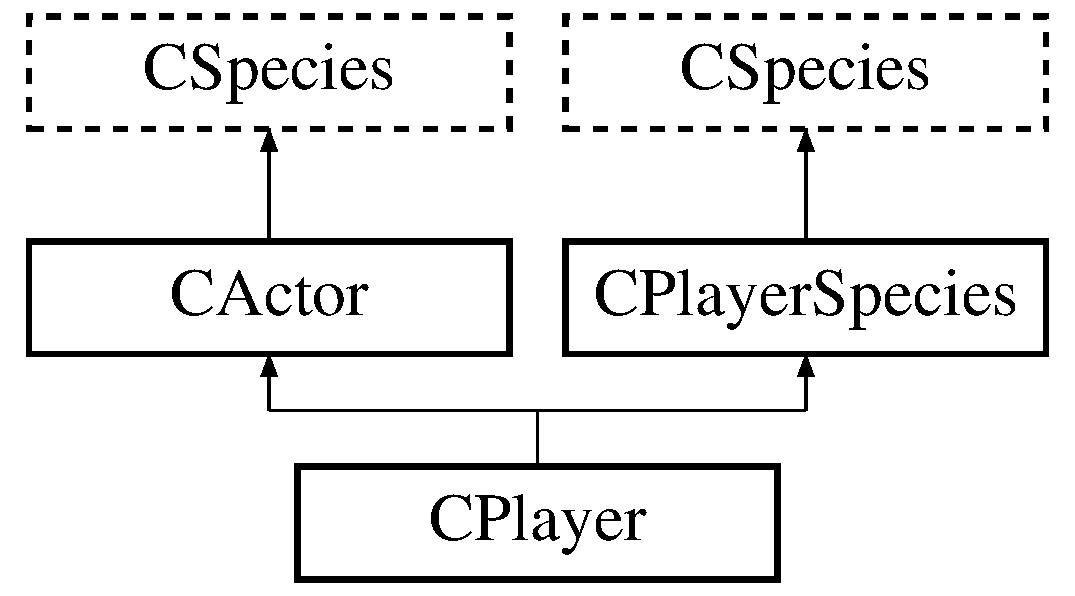
\includegraphics[height=3.000000cm]{class_c_player}
\end{center}
\end{figure}
\subsection*{Public Member Functions}
\begin{DoxyCompactItemize}
\item 
{\bfseries C\+Player} (const \hyperlink{class_c_player_species}{C\+Player\+Species} \&obj)\hypertarget{class_c_player_aa26b603893b75ea41882ea9faaa03978}{}\label{class_c_player_aa26b603893b75ea41882ea9faaa03978}

\item 
void {\bfseries Create\+Battle\+Menu} (std\+::vector$<$ std\+::string $>$ \+\_\+battle\+Item\+List)\hypertarget{class_c_player_a0d8f2a1b9b78c52bf7bae019079088ef}{}\label{class_c_player_a0d8f2a1b9b78c52bf7bae019079088ef}

\item 
void \hyperlink{class_c_player_a35f11b073c55586f3ef7b4eba4e82e27}{Draw} (int \+\_\+dx=0, int \+\_\+dy=0)
\item 
void {\bfseries Mp\+Heal} (int \+\_\+count)\hypertarget{class_c_player_a6889c018e8641105df56f21af8d1f5cb}{}\label{class_c_player_a6889c018e8641105df56f21af8d1f5cb}

\end{DoxyCompactItemize}
\subsection*{Additional Inherited Members}


\subsection{Member Function Documentation}
\index{C\+Player@{C\+Player}!Draw@{Draw}}
\index{Draw@{Draw}!C\+Player@{C\+Player}}
\subsubsection[{\texorpdfstring{Draw(int \+\_\+dx=0, int \+\_\+dy=0)}{Draw(int _dx=0, int _dy=0)}}]{\setlength{\rightskip}{0pt plus 5cm}void C\+Player\+::\+Draw (
\begin{DoxyParamCaption}
\item[{int}]{\+\_\+dx = {\ttfamily 0}, }
\item[{int}]{\+\_\+dy = {\ttfamily 0}}
\end{DoxyParamCaption}
)\hspace{0.3cm}{\ttfamily [virtual]}}\hypertarget{class_c_player_a35f11b073c55586f3ef7b4eba4e82e27}{}\label{class_c_player_a35f11b073c55586f3ef7b4eba4e82e27}
死亡演出/////////////////////////////////////////////////// 

Implements \hyperlink{class_c_actor}{C\+Actor}.



The documentation for this class was generated from the following files\+:\begin{DoxyCompactItemize}
\item 
Classes/Player.\+h\item 
Classes/Player.\+cpp\end{DoxyCompactItemize}

\hypertarget{class_c_player_species}{}\section{C\+Player\+Species Class Reference}
\label{class_c_player_species}\index{C\+Player\+Species@{C\+Player\+Species}}
Inheritance diagram for C\+Player\+Species\+:\begin{figure}[H]
\begin{center}
\leavevmode
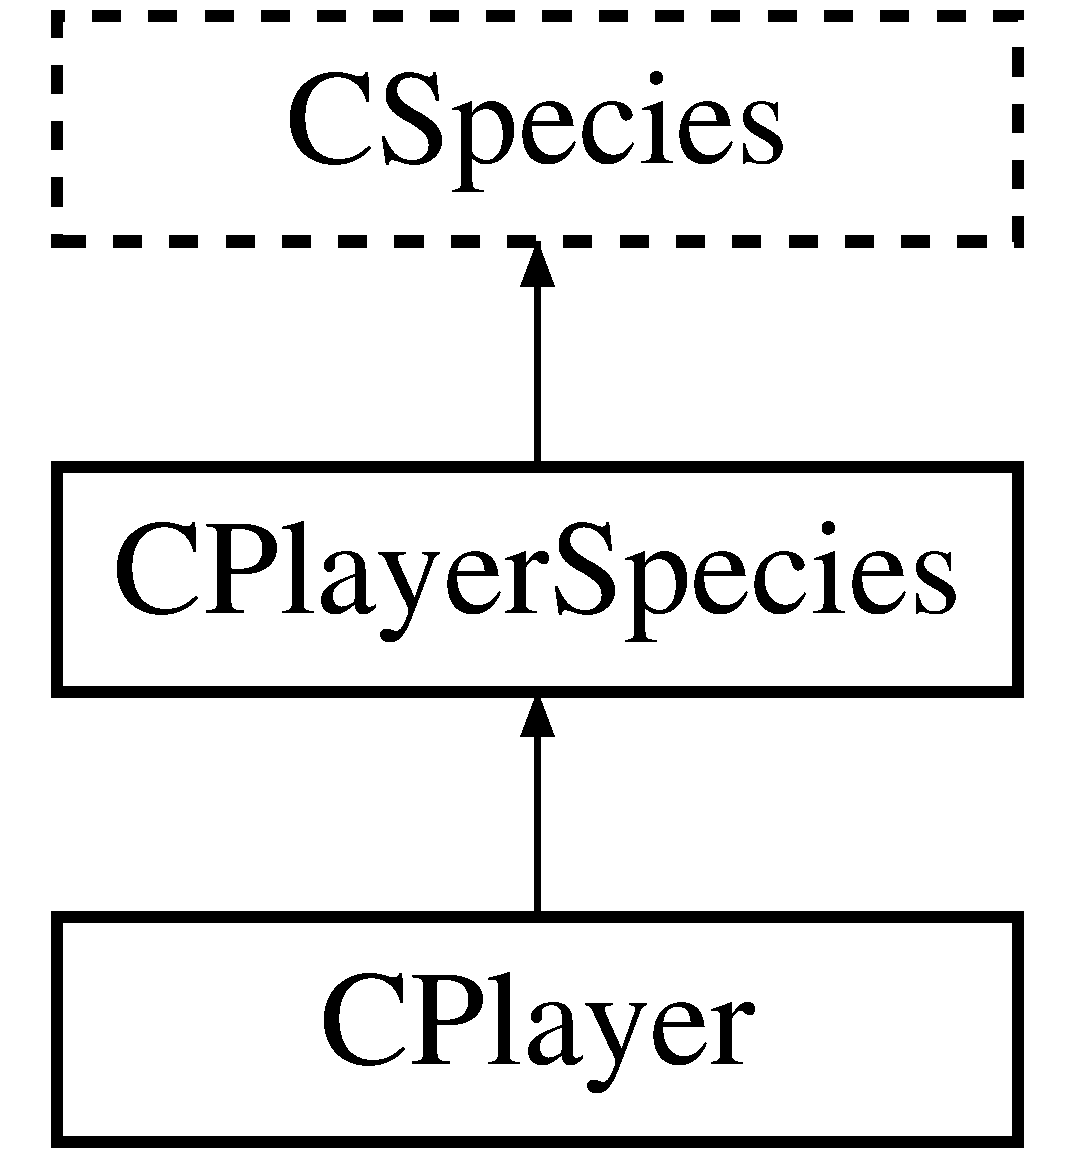
\includegraphics[height=3.000000cm]{class_c_player_species}
\end{center}
\end{figure}
\subsection*{Public Member Functions}
\begin{DoxyCompactItemize}
\item 
{\bfseries C\+Player\+Species} (const \hyperlink{class_c_player_species}{C\+Player\+Species} \&obj)\hypertarget{class_c_player_species_ad79929e7940087a6725f58b227afb027}{}\label{class_c_player_species_ad79929e7940087a6725f58b227afb027}

\end{DoxyCompactItemize}
\subsection*{Protected Attributes}
\begin{DoxyCompactItemize}
\item 
int {\bfseries Magic\+Count}\hypertarget{class_c_player_species_aaf73192bfdffa9a5bc6003f049a8edf4}{}\label{class_c_player_species_aaf73192bfdffa9a5bc6003f049a8edf4}

\item 
\hyperlink{structtrick__tag}{trick\+\_\+tag} {\bfseries Base\+Trick}\hypertarget{class_c_player_species_a2e68bce8c6d6db92809af315292fe760}{}\label{class_c_player_species_a2e68bce8c6d6db92809af315292fe760}

\item 
int {\bfseries Base\+Trick\+Power\+Gene}\hypertarget{class_c_player_species_ae49ffba3c0a43c008acc5dbe4a866f0f}{}\label{class_c_player_species_ae49ffba3c0a43c008acc5dbe4a866f0f}

\item 
std\+::string {\bfseries Accessory\+List} \mbox{[}M\+A\+X\+\_\+\+A\+C\+C\+E\+S\+S\+O\+R\+Y\+\_\+\+S\+L\+OT\mbox{]}\hypertarget{class_c_player_species_a77116b28f1f04ff5642b2c583d6a35d3}{}\label{class_c_player_species_a77116b28f1f04ff5642b2c583d6a35d3}

\end{DoxyCompactItemize}
\subsection*{Friends}
\begin{DoxyCompactItemize}
\item 
class {\bfseries C\+Player\+Species\+Manager}\hypertarget{class_c_player_species_a1f648829e43a62ea352129f6d9f96a7b}{}\label{class_c_player_species_a1f648829e43a62ea352129f6d9f96a7b}

\end{DoxyCompactItemize}
\subsection*{Additional Inherited Members}


The documentation for this class was generated from the following file\+:\begin{DoxyCompactItemize}
\item 
Classes/Species.\+h\end{DoxyCompactItemize}

\hypertarget{class_c_player_species_manager}{}\section{C\+Player\+Species\+Manager Class Reference}
\label{class_c_player_species_manager}\index{C\+Player\+Species\+Manager@{C\+Player\+Species\+Manager}}
\subsection*{Public Member Functions}
\begin{DoxyCompactItemize}
\item 
void {\bfseries Clear} ()\hypertarget{class_c_player_species_manager_a2747a6543b5bd8529123fa166703b155}{}\label{class_c_player_species_manager_a2747a6543b5bd8529123fa166703b155}

\item 
bool {\bfseries Check\+After\+Load} ()\hypertarget{class_c_player_species_manager_a5832677e2570cc8dc99706a4fda1cb01}{}\label{class_c_player_species_manager_a5832677e2570cc8dc99706a4fda1cb01}

\item 
bool {\bfseries Create\+Species} (const char $\ast$\+\_\+name, int \+\_\+level, int \+\_\+gene\+Max\+Hp, int \+\_\+gene\+Base\+Trick\+Power, int \+\_\+gene\+Atk, int \+\_\+gene\+Def, int \+\_\+gene\+Spd, int \+\_\+img, const \hyperlink{structtrick__tag}{trick\+\_\+tag} $\ast$\+\_\+base\+Trick)\hypertarget{class_c_player_species_manager_a1447a4fa34a4f59e6c3c1dba92d70a1d}{}\label{class_c_player_species_manager_a1447a4fa34a4f59e6c3c1dba92d70a1d}

\item 
bool {\bfseries Set\+Trick\+List} (const char $\ast$\+\_\+name, std\+::vector$<$ \hyperlink{structtrick__tag}{trick\+\_\+tag} const $\ast$ $>$ \+\_\+trick\+List)\hypertarget{class_c_player_species_manager_ae69493f939538606bfa6195e14fb4769}{}\label{class_c_player_species_manager_ae69493f939538606bfa6195e14fb4769}

\item 
\hyperlink{class_c_player_species}{C\+Player\+Species} $\ast$ {\bfseries Get\+Species} (const char $\ast$\+\_\+name)\hypertarget{class_c_player_species_manager_a46a6df63e45579a5aae2f62a43c31b7a}{}\label{class_c_player_species_manager_a46a6df63e45579a5aae2f62a43c31b7a}

\item 
\hyperlink{class_c_player_species}{C\+Player\+Species} $\ast$ {\bfseries Get\+Species} (int \+\_\+index)\hypertarget{class_c_player_species_manager_a599e0f12ce94ef42a6be176f9abdfaaa}{}\label{class_c_player_species_manager_a599e0f12ce94ef42a6be176f9abdfaaa}

\item 
bool {\bfseries Set\+Member\+List} (int \+\_\+index, const char $\ast$\+\_\+name)\hypertarget{class_c_player_species_manager_a4da79d2e642e76cd9c8751c0c7b588a4}{}\label{class_c_player_species_manager_a4da79d2e642e76cd9c8751c0c7b588a4}

\item 
bool {\bfseries Set\+Member\+List} ()\hypertarget{class_c_player_species_manager_a5f040b572abdf718340814149ed8a164}{}\label{class_c_player_species_manager_a5f040b572abdf718340814149ed8a164}

\item 
int {\bfseries Get\+Member\+List\+Size} () const \hypertarget{class_c_player_species_manager_a977388c23d3f42f25bca2b4035e3ba92}{}\label{class_c_player_species_manager_a977388c23d3f42f25bca2b4035e3ba92}

\item 
void {\bfseries Copy\+Value} (int P\+L\+A\+Y\+E\+R\+\_\+\+N\+UM, \hyperlink{class_c_player}{C\+Player} $\ast$\+\_\+player)\hypertarget{class_c_player_species_manager_a9dcebaabd5feb461dae6f8b7ddb0d0dd}{}\label{class_c_player_species_manager_a9dcebaabd5feb461dae6f8b7ddb0d0dd}

\item 
void {\bfseries Add\+Exp} (int \+\_\+exp)\hypertarget{class_c_player_species_manager_a270ce50fe517ad750b6b98a93e2140d5}{}\label{class_c_player_species_manager_a270ce50fe517ad750b6b98a93e2140d5}

\item 
bool {\bfseries Set\+Accessory} (std\+::string \+\_\+player\+Name, int \+\_\+slot, std\+::string \+\_\+accessory\+Item\+Name)\hypertarget{class_c_player_species_manager_abd020befdb5aff30407fa40987d4a164}{}\label{class_c_player_species_manager_abd020befdb5aff30407fa40987d4a164}

\item 
\hyperlink{class_c_accessory_item}{C\+Accessory\+Item} $\ast$ {\bfseries Get\+Accessory} (std\+::string \+\_\+player\+Name, int \+\_\+slot)\hypertarget{class_c_player_species_manager_af10e66b4500bec2bfc56deeee0e64d05}{}\label{class_c_player_species_manager_af10e66b4500bec2bfc56deeee0e64d05}

\end{DoxyCompactItemize}
\subsection*{Static Public Member Functions}
\begin{DoxyCompactItemize}
\item 
static \hyperlink{class_c_player_species_manager}{C\+Player\+Species\+Manager} $\ast$ {\bfseries Get\+Instance} ()\hypertarget{class_c_player_species_manager_a6141d74620bc72c22542ba19ee064a2c}{}\label{class_c_player_species_manager_a6141d74620bc72c22542ba19ee064a2c}

\end{DoxyCompactItemize}


The documentation for this class was generated from the following files\+:\begin{DoxyCompactItemize}
\item 
Classes/Player\+Species\+Manager.\+h\item 
Classes/Player\+Species\+Manager.\+cpp\end{DoxyCompactItemize}

\hypertarget{class_c_rect}{}\section{C\+Rect Class Reference}
\label{class_c_rect}\index{C\+Rect@{C\+Rect}}


二次元\+B\+O\+Xクラス////////////////////////////////////////  




{\ttfamily \#include $<$nunu\+Lib.\+h$>$}

\subsection*{Public Member Functions}
\begin{DoxyCompactItemize}
\item 
{\bfseries C\+Rect} (int \+\_\+left, int \+\_\+right, int \+\_\+top, int \+\_\+bottom)\hypertarget{class_c_rect_aa7328a334aa6519f731e55b185d9a75d}{}\label{class_c_rect_aa7328a334aa6519f731e55b185d9a75d}

\item 
\hyperlink{class_c_vector}{C\+Vector} {\bfseries Center} ()\hypertarget{class_c_rect_ad19e26519993f258cf7030cd8dffb95e}{}\label{class_c_rect_ad19e26519993f258cf7030cd8dffb95e}

\item 
int {\bfseries Width} ()\hypertarget{class_c_rect_ae1eed1eed18eaf90f1850f0cc2b4ee5c}{}\label{class_c_rect_ae1eed1eed18eaf90f1850f0cc2b4ee5c}

\item 
int {\bfseries Height} ()\hypertarget{class_c_rect_a25280cc1438c30f7d71f7adc19584a7e}{}\label{class_c_rect_a25280cc1438c30f7d71f7adc19584a7e}

\item 
void {\bfseries Set\+Width} (int \+\_\+width)\hypertarget{class_c_rect_a8daaae317869f628de3b55072337ff33}{}\label{class_c_rect_a8daaae317869f628de3b55072337ff33}

\item 
void {\bfseries Set\+Height} (int \+\_\+height)\hypertarget{class_c_rect_a7bdc8877386727761bf1d7954b9a8edd}{}\label{class_c_rect_a7bdc8877386727761bf1d7954b9a8edd}

\end{DoxyCompactItemize}
\subsection*{Public Attributes}
\begin{DoxyCompactItemize}
\item 
int {\bfseries Top}\hypertarget{class_c_rect_acd514ebe4843ae49ae3a02da7c18546e}{}\label{class_c_rect_acd514ebe4843ae49ae3a02da7c18546e}

\item 
int {\bfseries Left}\hypertarget{class_c_rect_afbeea9a97235280389aba0cc881a1d22}{}\label{class_c_rect_afbeea9a97235280389aba0cc881a1d22}

\item 
int {\bfseries Bottom}\hypertarget{class_c_rect_a13fe0739f59e06cb5a2ab4a4465b2343}{}\label{class_c_rect_a13fe0739f59e06cb5a2ab4a4465b2343}

\item 
int {\bfseries Right}\hypertarget{class_c_rect_aef5f621e8db98b4e61ba8d0e9816fff5}{}\label{class_c_rect_aef5f621e8db98b4e61ba8d0e9816fff5}

\end{DoxyCompactItemize}


\subsection{Detailed Description}
二次元\+B\+O\+Xクラス//////////////////////////////////////// 

The documentation for this class was generated from the following file\+:\begin{DoxyCompactItemize}
\item 
Classes/nunu\+Lib.\+h\end{DoxyCompactItemize}

\hypertarget{class_c_screen_changer}{}\section{C\+Screen\+Changer Class Reference}
\label{class_c_screen_changer}\index{C\+Screen\+Changer@{C\+Screen\+Changer}}
\subsection*{Public Types}
\begin{DoxyCompactItemize}
\item 
enum {\bfseries screenchange\+\_\+tag} \{ {\bfseries S\+C\+R\+E\+E\+N\+\_\+\+F\+A\+DE}, 
{\bfseries S\+C\+R\+E\+E\+N\+\_\+\+B\+O\+K\+A\+S\+HI}, 
{\bfseries S\+C\+R\+E\+E\+N\+\_\+\+G\+U\+R\+U\+G\+U\+RU}, 
{\bfseries S\+C\+R\+E\+E\+N\+\_\+\+N\+UM}
 \}\hypertarget{class_c_screen_changer_a8188a4717947ff55d37a920c36d197fc}{}\label{class_c_screen_changer_a8188a4717947ff55d37a920c36d197fc}

\end{DoxyCompactItemize}
\subsection*{Static Public Member Functions}
\begin{DoxyCompactItemize}
\item 
static void {\bfseries Change\+Screen} (const int \+\_\+p\+Graph, const int \+\_\+n\+Graph, const screenchange\+\_\+tag \+\_\+type, int \+\_\+count, int \+\_\+option=-\/1)\hypertarget{class_c_screen_changer_a95a7d23f355e888644665b848ba92eab}{}\label{class_c_screen_changer_a95a7d23f355e888644665b848ba92eab}

\end{DoxyCompactItemize}


The documentation for this class was generated from the following files\+:\begin{DoxyCompactItemize}
\item 
Classes/Screen\+Changer.\+h\item 
Classes/Screen\+Changer.\+cpp\end{DoxyCompactItemize}

\hypertarget{class_c_shop_manager}{}\section{C\+Shop\+Manager Class Reference}
\label{class_c_shop_manager}\index{C\+Shop\+Manager@{C\+Shop\+Manager}}
Inheritance diagram for C\+Shop\+Manager\+:\begin{figure}[H]
\begin{center}
\leavevmode
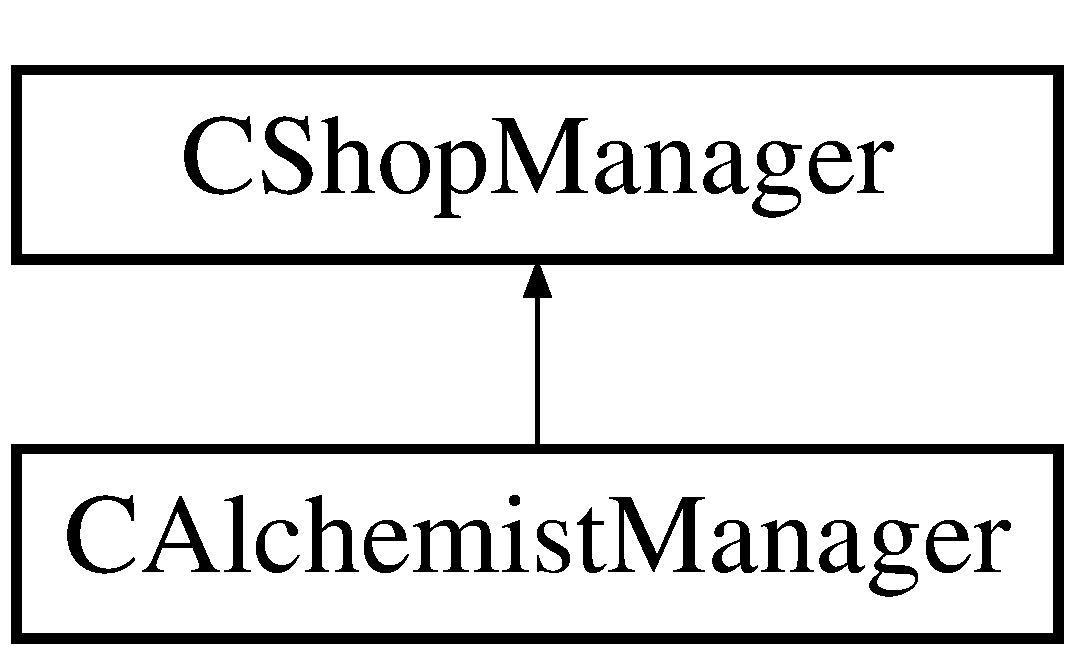
\includegraphics[height=2.000000cm]{class_c_shop_manager}
\end{center}
\end{figure}
\subsection*{Public Member Functions}
\begin{DoxyCompactItemize}
\item 
virtual void {\bfseries Init} ()\hypertarget{class_c_shop_manager_ac9b4db61b164eeb2d1179ba25c8b789e}{}\label{class_c_shop_manager_ac9b4db61b164eeb2d1179ba25c8b789e}

\item 
virtual bool {\bfseries Open\+Shop} (int \+\_\+index)\hypertarget{class_c_shop_manager_a5eed1bcf7e2f3682233a9409410bb4d8}{}\label{class_c_shop_manager_a5eed1bcf7e2f3682233a9409410bb4d8}

\item 
bool {\bfseries Main} ()\hypertarget{class_c_shop_manager_a9bad8f0e9744a624d7afece9f89521fc}{}\label{class_c_shop_manager_a9bad8f0e9744a624d7afece9f89521fc}

\item 
bool {\bfseries Add\+Shop} (int \+\_\+index, std\+::vector$<$ std\+::string $>$ \+\_\+item\+List)\hypertarget{class_c_shop_manager_aa6d2584f142db1ab60d84a96c3d0a06c}{}\label{class_c_shop_manager_aa6d2584f142db1ab60d84a96c3d0a06c}

\item 
std\+::vector$<$ std\+::string $>$ {\bfseries Get\+Shop} (int \+\_\+index)\hypertarget{class_c_shop_manager_a54ca0cef8d7ae6fe90f174f42b9d2846}{}\label{class_c_shop_manager_a54ca0cef8d7ae6fe90f174f42b9d2846}

\item 
bool {\bfseries Is\+Open} ()\hypertarget{class_c_shop_manager_ac6abebd722efe82d578ff6d72879628d}{}\label{class_c_shop_manager_ac6abebd722efe82d578ff6d72879628d}

\item 
void {\bfseries Draw} ()\hypertarget{class_c_shop_manager_ab64860e553b73fc75f6585aeb77b57f3}{}\label{class_c_shop_manager_ab64860e553b73fc75f6585aeb77b57f3}

\end{DoxyCompactItemize}
\subsection*{Static Public Member Functions}
\begin{DoxyCompactItemize}
\item 
static \hyperlink{class_c_shop_manager}{C\+Shop\+Manager} $\ast$ {\bfseries Get\+Instance} ()\hypertarget{class_c_shop_manager_ae312c7619ac9a9e80f9e539923aa3957}{}\label{class_c_shop_manager_ae312c7619ac9a9e80f9e539923aa3957}

\end{DoxyCompactItemize}
\subsection*{Protected Member Functions}
\begin{DoxyCompactItemize}
\item 
{\bfseries C\+Shop\+Manager} (const \hyperlink{class_c_shop_manager}{C\+Shop\+Manager} \&hoge)\hypertarget{class_c_shop_manager_a60216d09d37b0f0d254494f0901720e9}{}\label{class_c_shop_manager_a60216d09d37b0f0d254494f0901720e9}

\item 
\hyperlink{class_c_shop_manager}{C\+Shop\+Manager} \& {\bfseries operator=} (const \hyperlink{class_c_shop_manager}{C\+Shop\+Manager} \&hoge)\hypertarget{class_c_shop_manager_a65deda8f79ea5691c63e2ceb4ab9b2b8}{}\label{class_c_shop_manager_a65deda8f79ea5691c63e2ceb4ab9b2b8}

\end{DoxyCompactItemize}
\subsection*{Protected Attributes}
\begin{DoxyCompactItemize}
\item 
std\+::map$<$ int, std\+::vector$<$ std\+::string $>$ $>$ {\bfseries Shop\+Bank}\hypertarget{class_c_shop_manager_a53009437909f484dafe64dd35aec1e0b}{}\label{class_c_shop_manager_a53009437909f484dafe64dd35aec1e0b}

\item 
int {\bfseries Current\+Open\+Shop\+Index}\hypertarget{class_c_shop_manager_ade3960a1bb8799a10414be657e7d461f}{}\label{class_c_shop_manager_ade3960a1bb8799a10414be657e7d461f}

\item 
\hyperlink{class_c_shop_menu}{C\+Shop\+Menu} $\ast$ {\bfseries Shop\+Menu}\hypertarget{class_c_shop_manager_afc6aa72e25cb31cac4fcb55c7d3c18d0}{}\label{class_c_shop_manager_afc6aa72e25cb31cac4fcb55c7d3c18d0}

\end{DoxyCompactItemize}


The documentation for this class was generated from the following files\+:\begin{DoxyCompactItemize}
\item 
Classes/Shop\+Manager.\+h\item 
Classes/Shop\+Manager.\+cpp\end{DoxyCompactItemize}

\hypertarget{class_c_shop_menu}{}\section{C\+Shop\+Menu Class Reference}
\label{class_c_shop_menu}\index{C\+Shop\+Menu@{C\+Shop\+Menu}}
Inheritance diagram for C\+Shop\+Menu\+:\begin{figure}[H]
\begin{center}
\leavevmode
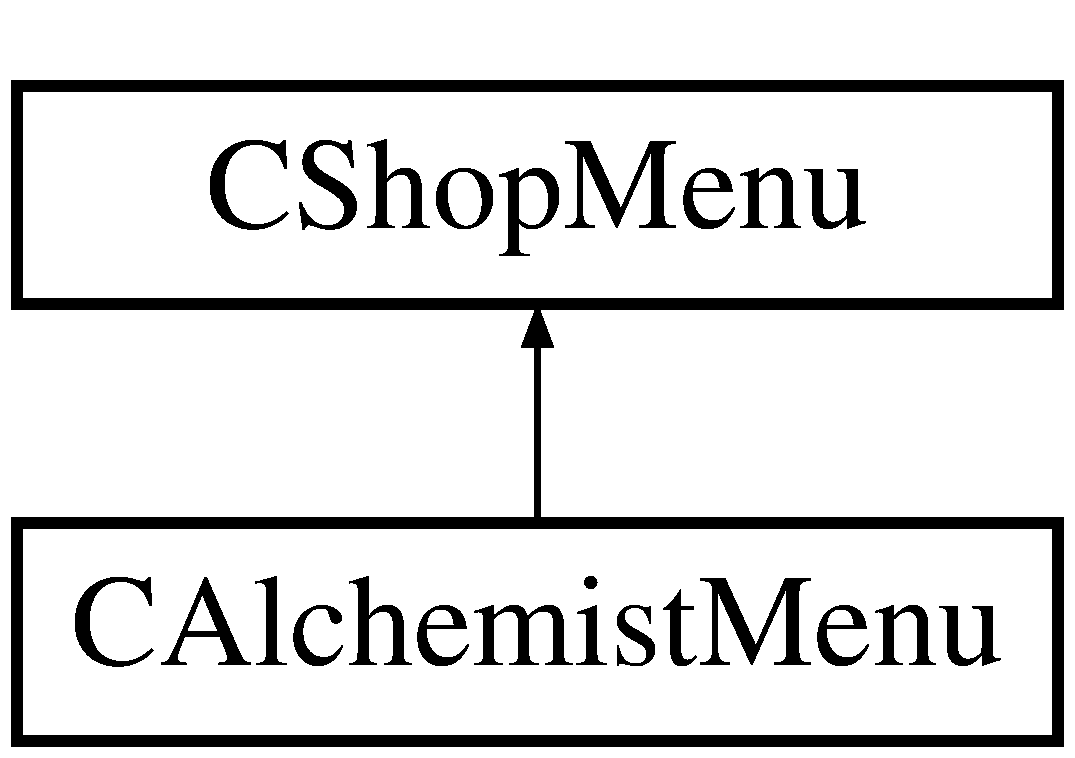
\includegraphics[height=2.000000cm]{class_c_shop_menu}
\end{center}
\end{figure}
\subsection*{Public Member Functions}
\begin{DoxyCompactItemize}
\item 
virtual void {\bfseries Move} (int \+\_\+dir)\hypertarget{class_c_shop_menu_ab30b209f6fee6e4b7c5ae71f6c8a3ab9}{}\label{class_c_shop_menu_ab30b209f6fee6e4b7c5ae71f6c8a3ab9}

\item 
virtual void {\bfseries Draw} ()\hypertarget{class_c_shop_menu_ac0ff02e1cf8a9bc30851a97f6d1d758a}{}\label{class_c_shop_menu_ac0ff02e1cf8a9bc30851a97f6d1d758a}

\item 
virtual bool {\bfseries Buy} ()\hypertarget{class_c_shop_menu_a848ae2ce17e81dc8a4c7b44cb5883a45}{}\label{class_c_shop_menu_a848ae2ce17e81dc8a4c7b44cb5883a45}

\item 
virtual bool {\bfseries Can\+Buy} ()\hypertarget{class_c_shop_menu_adf8f8f2be599d4149a302d516e12105c}{}\label{class_c_shop_menu_adf8f8f2be599d4149a302d516e12105c}

\item 
virtual bool {\bfseries Can\+Close} ()\hypertarget{class_c_shop_menu_adb6bd28f67d5ceede013f21e1bddee06}{}\label{class_c_shop_menu_adb6bd28f67d5ceede013f21e1bddee06}

\end{DoxyCompactItemize}
\subsection*{Public Attributes}
\begin{DoxyCompactItemize}
\item 
std\+::vector$<$ \hyperlink{class_c_item}{C\+Item} $\ast$ $>$ {\bfseries Item\+List}\hypertarget{class_c_shop_menu_af2770e04cbb5c34641a5dd73f81fe33d}{}\label{class_c_shop_menu_af2770e04cbb5c34641a5dd73f81fe33d}

\item 
std\+::vector$<$ int $>$ {\bfseries Basket}\hypertarget{class_c_shop_menu_a1094513959ee729ca1afadc5aeda73ff}{}\label{class_c_shop_menu_a1094513959ee729ca1afadc5aeda73ff}

\item 
int {\bfseries Sum\+Price}\hypertarget{class_c_shop_menu_a5dba1be33be60e2dafa22f37cfa72c73}{}\label{class_c_shop_menu_a5dba1be33be60e2dafa22f37cfa72c73}

\item 
int {\bfseries Cursor}\hypertarget{class_c_shop_menu_a509758e399dbda43cc718b6fc7c83e9c}{}\label{class_c_shop_menu_a509758e399dbda43cc718b6fc7c83e9c}

\item 
bool {\bfseries Is\+Confirm}\hypertarget{class_c_shop_menu_a2d644595fcab08f8bc5d51e5a383fef3}{}\label{class_c_shop_menu_a2d644595fcab08f8bc5d51e5a383fef3}

\item 
\hyperlink{class_c_item_manager}{C\+Item\+Manager} $\ast$ {\bfseries Item\+Manager}\hypertarget{class_c_shop_menu_a3c6b837edc5c90e2f9e647489ab48e35}{}\label{class_c_shop_menu_a3c6b837edc5c90e2f9e647489ab48e35}

\end{DoxyCompactItemize}


The documentation for this class was generated from the following files\+:\begin{DoxyCompactItemize}
\item 
Classes/Shop\+Manager.\+h\item 
Classes/Shop\+Manager.\+cpp\end{DoxyCompactItemize}

\hypertarget{class_c_species}{}\section{C\+Species Class Reference}
\label{class_c_species}\index{C\+Species@{C\+Species}}
Inheritance diagram for C\+Species\+:\begin{figure}[H]
\begin{center}
\leavevmode
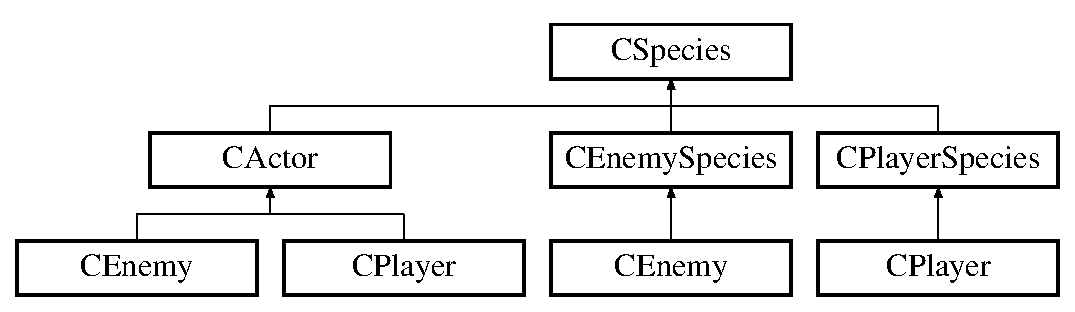
\includegraphics[height=3.000000cm]{class_c_species}
\end{center}
\end{figure}
\subsection*{Public Member Functions}
\begin{DoxyCompactItemize}
\item 
std\+::string {\bfseries Get\+Name} () const \hypertarget{class_c_species_a8fc218299b0b0d2635538f2caff84207}{}\label{class_c_species_a8fc218299b0b0d2635538f2caff84207}

\item 
int {\bfseries Get\+Level} ()\hypertarget{class_c_species_a16e911c3b7c52084d5dff8e187fb575f}{}\label{class_c_species_a16e911c3b7c52084d5dff8e187fb575f}

\end{DoxyCompactItemize}
\subsection*{Protected Member Functions}
\begin{DoxyCompactItemize}
\item 
void {\bfseries Set\+Value} (const char $\ast$\+\_\+name, int \+\_\+level, int \+\_\+gene\+Max\+Hp, int \+\_\+gene\+Atk, int \+\_\+gene\+Def, int \+\_\+gene\+Spd)\hypertarget{class_c_species_afddefbaaa3ff47530114b4816be0665d}{}\label{class_c_species_afddefbaaa3ff47530114b4816be0665d}

\end{DoxyCompactItemize}
\subsection*{Protected Attributes}
\begin{DoxyCompactItemize}
\item 
std\+::string {\bfseries Name}\hypertarget{class_c_species_a4ae49cfe79de97715fae5c6f4a248ba3}{}\label{class_c_species_a4ae49cfe79de97715fae5c6f4a248ba3}

\item 
int {\bfseries Img}\hypertarget{class_c_species_a9b2d09eec23e334706990b4c03056483}{}\label{class_c_species_a9b2d09eec23e334706990b4c03056483}

\item 
int {\bfseries Level}\hypertarget{class_c_species_a9312314cc7998f560b62b7dd7f630997}{}\label{class_c_species_a9312314cc7998f560b62b7dd7f630997}

\item 
int {\bfseries Hp}\hypertarget{class_c_species_a864428128364ef09a49bab0a15e0a9ad}{}\label{class_c_species_a864428128364ef09a49bab0a15e0a9ad}

\item 
int {\bfseries Max\+Hp\+Gene}\hypertarget{class_c_species_af8936d33bbf9d4b21918f84943e23813}{}\label{class_c_species_af8936d33bbf9d4b21918f84943e23813}

\item 
int {\bfseries Atk\+Gene}\hypertarget{class_c_species_a66431b002abfd87d4b30f180a46e5e47}{}\label{class_c_species_a66431b002abfd87d4b30f180a46e5e47}

\item 
int {\bfseries Def\+Gene}\hypertarget{class_c_species_a9d1e9f6a98b9e321a82af8cd5ee171b3}{}\label{class_c_species_a9d1e9f6a98b9e321a82af8cd5ee171b3}

\item 
int {\bfseries Spd\+Gene}\hypertarget{class_c_species_a9e1fa2d1be4e70d7a5a701c15d21dfcb}{}\label{class_c_species_a9e1fa2d1be4e70d7a5a701c15d21dfcb}

\item 
std\+::vector$<$ \hyperlink{structtrick__tag}{trick\+\_\+tag} const $\ast$ $>$ {\bfseries Trick\+List}\hypertarget{class_c_species_a5d7cb8805a1f0d8f28280ae62ed4421d}{}\label{class_c_species_a5d7cb8805a1f0d8f28280ae62ed4421d}

\end{DoxyCompactItemize}


The documentation for this class was generated from the following files\+:\begin{DoxyCompactItemize}
\item 
Classes/Species.\+h\item 
Classes/Species.\+cpp\end{DoxyCompactItemize}

\hypertarget{class_c_talk_name}{}\section{C\+Talk\+Name Class Reference}
\label{class_c_talk_name}\index{C\+Talk\+Name@{C\+Talk\+Name}}
\subsection*{Public Types}
\begin{DoxyCompactItemize}
\item 
enum \{ {\bfseries S\+I\+D\+E\+\_\+\+N\+UM} =2, 
{\bfseries N\+A\+M\+E\+\_\+\+N\+UM} =10
 \}\hypertarget{class_c_talk_name_ab2a838e591222eaa9cd4e64859d5a237}{}\label{class_c_talk_name_ab2a838e591222eaa9cd4e64859d5a237}

\end{DoxyCompactItemize}
\subsection*{Public Member Functions}
\begin{DoxyCompactItemize}
\item 
void {\bfseries Init} ()\hypertarget{class_c_talk_name_a3ef60366e54f087ce720012e49413989}{}\label{class_c_talk_name_a3ef60366e54f087ce720012e49413989}

\item 
void {\bfseries Clear} (bool \+\_\+left)\hypertarget{class_c_talk_name_a0882a63ec1fbb6baf7dc35e8db8946de}{}\label{class_c_talk_name_a0882a63ec1fbb6baf7dc35e8db8946de}

\item 
bool {\bfseries Add} (bool \+\_\+left, int \+\_\+num,...)\hypertarget{class_c_talk_name_a1ac94e10cca5b4fb684f1800c71ec51d}{}\label{class_c_talk_name_a1ac94e10cca5b4fb684f1800c71ec51d}

\item 
bool {\bfseries Dec} (bool \+\_\+left, int \+\_\+num,...)\hypertarget{class_c_talk_name_a38910b8d0c6d1ee35a1dc2fa67630d5d}{}\label{class_c_talk_name_a38910b8d0c6d1ee35a1dc2fa67630d5d}

\item 
bool {\bfseries Set\+Now\+Name} (bool \+\_\+left, char $\ast$\+\_\+name, bool \+\_\+add=true)\hypertarget{class_c_talk_name_a1d280a5685ffefc80f7e34347d8aa215}{}\label{class_c_talk_name_a1d280a5685ffefc80f7e34347d8aa215}

\item 
void {\bfseries Set\+Now\+Side} (bool \+\_\+left)\hypertarget{class_c_talk_name_a640f64ba2f900dbdfedc5b7e0b0aaec5}{}\label{class_c_talk_name_a640f64ba2f900dbdfedc5b7e0b0aaec5}

\item 
bool {\bfseries Get\+Visible} ()\hypertarget{class_c_talk_name_af817792d95d0deb8f0fe3456919d1dc9}{}\label{class_c_talk_name_af817792d95d0deb8f0fe3456919d1dc9}

\item 
std\+::string {\bfseries Get\+Now\+Name} ()\hypertarget{class_c_talk_name_a840c6c6f458f56bda0926f5a1cad1df9}{}\label{class_c_talk_name_a840c6c6f458f56bda0926f5a1cad1df9}

\item 
void {\bfseries Draw} (int \+\_\+left, int \+\_\+right, int bottom)\hypertarget{class_c_talk_name_a1a86af6032c1119ae1ce754a9ef7bd95}{}\label{class_c_talk_name_a1a86af6032c1119ae1ce754a9ef7bd95}

\end{DoxyCompactItemize}


The documentation for this class was generated from the following files\+:\begin{DoxyCompactItemize}
\item 
Classes/Talk\+Name.\+h\item 
Classes/Talk\+Name.\+cpp\end{DoxyCompactItemize}

\hypertarget{class_c_battle_1_1_c_target_marker}{}\section{C\+Battle\+:\+:C\+Target\+Marker Class Reference}
\label{class_c_battle_1_1_c_target_marker}\index{C\+Battle\+::\+C\+Target\+Marker@{C\+Battle\+::\+C\+Target\+Marker}}
\subsection*{Public Member Functions}
\begin{DoxyCompactItemize}
\item 
void {\bfseries Set\+Image} (int \+\_\+img)\hypertarget{class_c_battle_1_1_c_target_marker_a768eef95ac308f399a2b241ab01285ab}{}\label{class_c_battle_1_1_c_target_marker_a768eef95ac308f399a2b241ab01285ab}

\item 
void {\bfseries Init} (int \+\_\+actornum, int \+\_\+playernum, int \+\_\+enemynum)\hypertarget{class_c_battle_1_1_c_target_marker_acd2713b509388985eb71c12da0020c2c}{}\label{class_c_battle_1_1_c_target_marker_acd2713b509388985eb71c12da0020c2c}

\item 
void {\bfseries Set\+Visible} (bool \+\_\+visible)\hypertarget{class_c_battle_1_1_c_target_marker_af1105a24b547b8c39aef1160d5df7871}{}\label{class_c_battle_1_1_c_target_marker_af1105a24b547b8c39aef1160d5df7871}

\item 
void {\bfseries Set\+Side} (bool \+\_\+enemy)\hypertarget{class_c_battle_1_1_c_target_marker_ac641dea3416e37314f028946608d5d97}{}\label{class_c_battle_1_1_c_target_marker_ac641dea3416e37314f028946608d5d97}

\item 
bool {\bfseries Get\+Side} ()\hypertarget{class_c_battle_1_1_c_target_marker_adc0e29f55095abe5ef7a3f9a4857030d}{}\label{class_c_battle_1_1_c_target_marker_adc0e29f55095abe5ef7a3f9a4857030d}

\item 
void {\bfseries Set\+Index} (int \+\_\+index)\hypertarget{class_c_battle_1_1_c_target_marker_aca1e3ece9c836d851077b5cd8ba57497}{}\label{class_c_battle_1_1_c_target_marker_aca1e3ece9c836d851077b5cd8ba57497}

\item 
void {\bfseries Set\+Dead\+Ok} (bool \+\_\+deadok)\hypertarget{class_c_battle_1_1_c_target_marker_ad760d3836d8e7bc111df170ce0c83e48}{}\label{class_c_battle_1_1_c_target_marker_ad760d3836d8e7bc111df170ce0c83e48}

\item 
void {\bfseries Check\+Now\+Index} (\hyperlink{class_c_battle}{C\+Battle} $\ast$\+\_\+battle)\hypertarget{class_c_battle_1_1_c_target_marker_a98d66637a90cc70b4b8597eaaa90115c}{}\label{class_c_battle_1_1_c_target_marker_a98d66637a90cc70b4b8597eaaa90115c}

\item 
void {\bfseries Move} (int \+\_\+dir, \hyperlink{class_c_battle}{C\+Battle} $\ast$\+\_\+battle, int \+\_\+count=0)\hypertarget{class_c_battle_1_1_c_target_marker_a18d3ef725310c1b767aeb982a57c9406}{}\label{class_c_battle_1_1_c_target_marker_a18d3ef725310c1b767aeb982a57c9406}

\item 
void {\bfseries Decide} (\hyperlink{class_c_battle}{C\+Battle} $\ast$\+\_\+battle, int \+\_\+actor\+Index)\hypertarget{class_c_battle_1_1_c_target_marker_a50bd363126ce97b9e8a07c1fcd58f903}{}\label{class_c_battle_1_1_c_target_marker_a50bd363126ce97b9e8a07c1fcd58f903}

\item 
void {\bfseries Draw} (int dx=0, int dy=0)\hypertarget{class_c_battle_1_1_c_target_marker_a8fe86f2f5aa3e189ff8a671095cc3eee}{}\label{class_c_battle_1_1_c_target_marker_a8fe86f2f5aa3e189ff8a671095cc3eee}

\end{DoxyCompactItemize}


The documentation for this class was generated from the following files\+:\begin{DoxyCompactItemize}
\item 
Classes/Battle.\+h\item 
Classes/Battle.\+cpp\end{DoxyCompactItemize}

\hypertarget{class_c_text_box}{}\section{C\+Text\+Box Class Reference}
\label{class_c_text_box}\index{C\+Text\+Box@{C\+Text\+Box}}
Inheritance diagram for C\+Text\+Box\+:\begin{figure}[H]
\begin{center}
\leavevmode
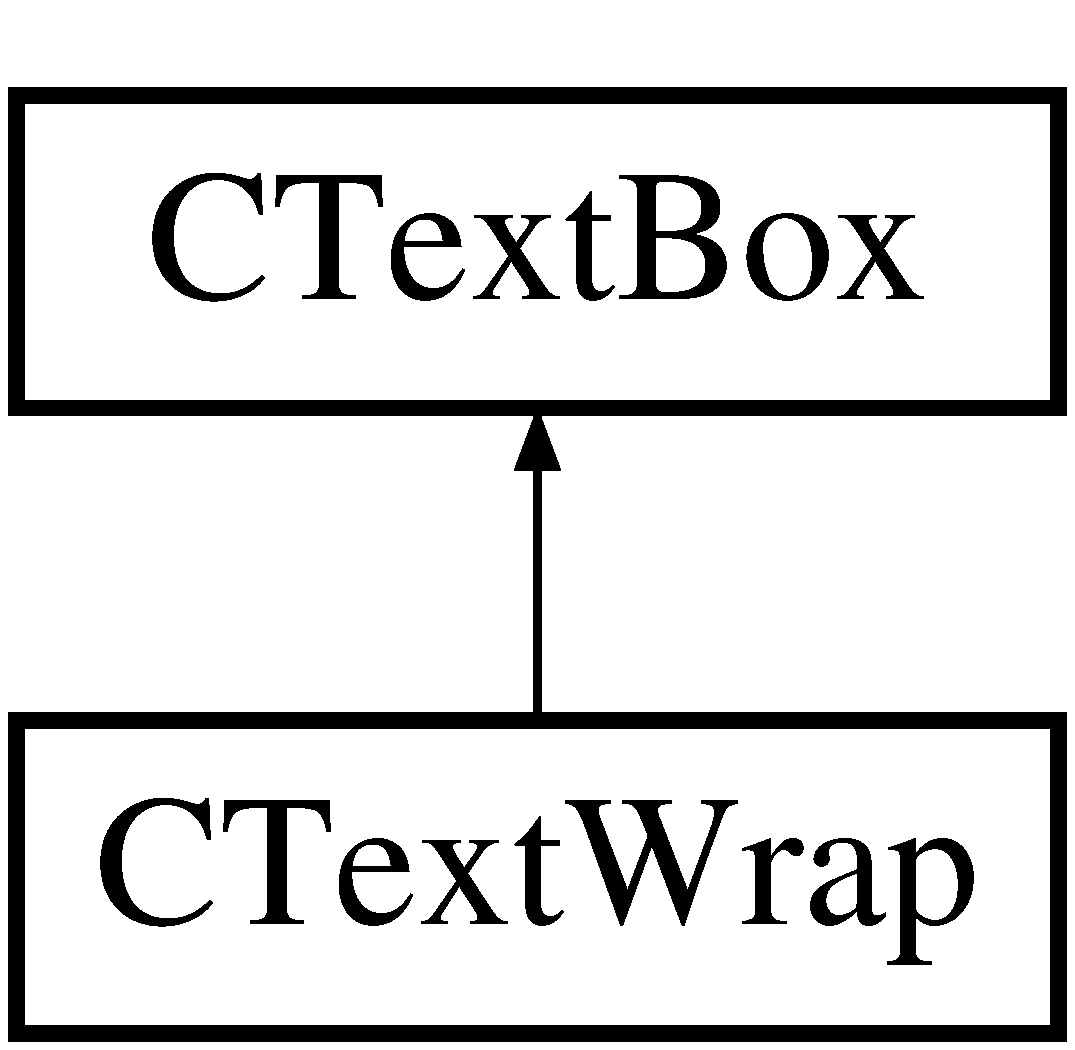
\includegraphics[height=2.000000cm]{class_c_text_box}
\end{center}
\end{figure}
\subsection*{Classes}
\begin{DoxyCompactItemize}
\item 
struct \hyperlink{struct_c_text_box_1_1ruby__tag}{ruby\+\_\+tag}
\end{DoxyCompactItemize}
\subsection*{Public Member Functions}
\begin{DoxyCompactItemize}
\item 
void {\bfseries Init} (int \+\_\+posx, int \+\_\+posy, int \+\_\+width, int \+\_\+height, int \+\_\+line, int \+\_\+words, int \+\_\+fontsize, int \+\_\+color1, int \+\_\+color2, int \+\_\+autoplayspeed, \hyperlink{class_c_field_log}{C\+Field\+Log} $\ast$\+\_\+log\+Window)\hypertarget{class_c_text_box_ad1e1baa450dce91e33d3d55de3db6f66}{}\label{class_c_text_box_ad1e1baa450dce91e33d3d55de3db6f66}

\item 
virtual void {\bfseries Term} (\hyperlink{class_c_cmd_list}{C\+Cmd\+List} $\ast$\+\_\+cmdlist)\hypertarget{class_c_text_box_a1cc1c4041f1c01dc807ae12fe5d67aef}{}\label{class_c_text_box_a1cc1c4041f1c01dc807ae12fe5d67aef}

\item 
bool {\bfseries Main} (\hyperlink{class_c_cmd_list}{C\+Cmd\+List} $\ast$\+\_\+cmdlist, \hyperlink{class_c_flag_set}{C\+Flag\+Set} $\ast$\+\_\+flagset)\hypertarget{class_c_text_box_a03fd29ccba104eb4728077ec505de351}{}\label{class_c_text_box_a03fd29ccba104eb4728077ec505de351}

\item 
virtual void {\bfseries Draw} (bool \+\_\+showingstop=false)\hypertarget{class_c_text_box_a37a13a78ccab5d554538a7289f654a3c}{}\label{class_c_text_box_a37a13a78ccab5d554538a7289f654a3c}

\item 
bool {\bfseries Add\+Stock} (char $\ast$String, int dir=D\+O\+WN, int count=-\/1)\hypertarget{class_c_text_box_a3f57fdc2e13a0f3e97a15df497bcee0d}{}\label{class_c_text_box_a3f57fdc2e13a0f3e97a15df497bcee0d}

\item 
bool {\bfseries Add\+Stock} (char $\ast$$\ast$String, int dir=D\+O\+WN, int count=-\/1)\hypertarget{class_c_text_box_a108213bf12542ecaf088e6fcbb3f8165}{}\label{class_c_text_box_a108213bf12542ecaf088e6fcbb3f8165}

\item 
void {\bfseries Next\+Page} (\hyperlink{class_c_cmd_list}{C\+Cmd\+List} $\ast$\+\_\+cmdlist, \hyperlink{class_c_flag_set}{C\+Flag\+Set} $\ast$\+\_\+flagset)\hypertarget{class_c_text_box_aa73ba00db6a70351678641c9b63afe3e}{}\label{class_c_text_box_aa73ba00db6a70351678641c9b63afe3e}

\item 
direction\+\_\+tag {\bfseries Get\+Original\+Dir} () const \hypertarget{class_c_text_box_a88c6bfe580409fd230e97eef4b459886}{}\label{class_c_text_box_a88c6bfe580409fd230e97eef4b459886}

\item 
void {\bfseries Set\+Visible} (bool \+\_\+visible)\hypertarget{class_c_text_box_a01bd248991cd8095c47e348eca428113}{}\label{class_c_text_box_a01bd248991cd8095c47e348eca428113}

\item 
void {\bfseries Set\+Return\+Visible} (bool \+\_\+visible)\hypertarget{class_c_text_box_ae1080ad7b6a0104a8cf0701072b3c321}{}\label{class_c_text_box_ae1080ad7b6a0104a8cf0701072b3c321}

\item 
void {\bfseries Set\+Auto\+Play} (bool \+\_\+autoplay, int \+\_\+autoplayspeed=N\+U\+LL)\hypertarget{class_c_text_box_ac8cab32e4d3c5b4e593b2ef23a727e67}{}\label{class_c_text_box_ac8cab32e4d3c5b4e593b2ef23a727e67}

\item 
void {\bfseries Log\+Talk\+Name} ()\hypertarget{class_c_text_box_a8c93524c2dab0e76bcdcbd417a77cbbb}{}\label{class_c_text_box_a8c93524c2dab0e76bcdcbd417a77cbbb}

\end{DoxyCompactItemize}
\subsection*{Public Attributes}
\begin{DoxyCompactItemize}
\item 
\hyperlink{class_c_talk_name}{C\+Talk\+Name} {\bfseries Talk\+Name}\hypertarget{class_c_text_box_a62c9ee81affb1b131ded9511c6c0d0aa}{}\label{class_c_text_box_a62c9ee81affb1b131ded9511c6c0d0aa}

\end{DoxyCompactItemize}
\subsection*{Protected Types}
\begin{DoxyCompactItemize}
\item 
enum \{ \\*
{\bfseries S\+T\+O\+C\+K\+\_\+\+L\+I\+N\+E\+\_\+\+N\+UM} = 1000, 
{\bfseries L\+I\+N\+E\+\_\+\+M\+AX} = 20, 
{\bfseries W\+O\+R\+D\+\_\+\+M\+AX} = 256, 
{\bfseries L\+I\+N\+E\+\_\+\+S\+P\+A\+CE} = 10, 
\\*
{\bfseries S\+H\+O\+W\+I\+N\+G\+\_\+\+S\+P\+E\+ED} = 80
 \}\hypertarget{class_c_text_box_a24f328ef4e8a4ff88cd202ca1505be59}{}\label{class_c_text_box_a24f328ef4e8a4ff88cd202ca1505be59}

\item 
enum \{ {\bfseries P\+A\+GE}
 \}\hypertarget{class_c_text_box_a242b47e9de734288cdd46fb1a93d2b39}{}\label{class_c_text_box_a242b47e9de734288cdd46fb1a93d2b39}

\end{DoxyCompactItemize}
\subsection*{Protected Member Functions}
\begin{DoxyCompactItemize}
\item 
void {\bfseries Stock\+Clear} ()\hypertarget{class_c_text_box_a85ef90b8276c375140f209720a43620c}{}\label{class_c_text_box_a85ef90b8276c375140f209720a43620c}

\item 
void {\bfseries Text\+Clear} ()\hypertarget{class_c_text_box_a4489f09f66d98d827023f931ea7e4d42}{}\label{class_c_text_box_a4489f09f66d98d827023f931ea7e4d42}

\item 
void {\bfseries Draw\+\_\+\+Animation} (bool \+\_\+showingstop)\hypertarget{class_c_text_box_aecc3d147864ce8f6db8da44beee94618}{}\label{class_c_text_box_aecc3d147864ce8f6db8da44beee94618}

\item 
void {\bfseries Draw\+\_\+\+Ruby} ()\hypertarget{class_c_text_box_aa666b4dec9d3fd299db68bd2079860e0}{}\label{class_c_text_box_aa666b4dec9d3fd299db68bd2079860e0}

\item 
bool {\bfseries Next\+Line} (\hyperlink{class_c_cmd_list}{C\+Cmd\+List} $\ast$\+\_\+cmdlist, \hyperlink{class_c_flag_set}{C\+Flag\+Set} $\ast$\+\_\+flagset)\hypertarget{class_c_text_box_a7b64cd62e3f9ae79df4b0712520f08a4}{}\label{class_c_text_box_a7b64cd62e3f9ae79df4b0712520f08a4}

\item 
bool {\bfseries Solve} (const char $\ast$string, \hyperlink{class_c_flag_set}{C\+Flag\+Set} $\ast$\+\_\+flagset)\hypertarget{class_c_text_box_a4b311191730cb9beaa9650ef9dc93774}{}\label{class_c_text_box_a4b311191730cb9beaa9650ef9dc93774}

\item 
void {\bfseries Arg\+Cut} (const char $\ast$\+\_\+string, char $\ast$$\ast$\&command, char $\ast$$\ast$\&arg, int \+\_\+argnum)\hypertarget{class_c_text_box_aed2ac0a94532d4ec17001bca21e8d22a}{}\label{class_c_text_box_aed2ac0a94532d4ec17001bca21e8d22a}

\item 
int {\bfseries Text\+Line\+Num} ()\hypertarget{class_c_text_box_aef9f285dc1b55c170f14b571f7b788de}{}\label{class_c_text_box_aef9f285dc1b55c170f14b571f7b788de}

\end{DoxyCompactItemize}
\subsection*{Protected Attributes}
\begin{DoxyCompactItemize}
\item 
char {\bfseries ch\+Stock} \mbox{[}S\+T\+O\+C\+K\+\_\+\+L\+I\+N\+E\+\_\+\+N\+UM\mbox{]}\mbox{[}W\+O\+R\+D\+\_\+\+M\+AX\mbox{]}\hypertarget{class_c_text_box_ab612e13e1e4952a2f48f0536f4f0c0e9}{}\label{class_c_text_box_ab612e13e1e4952a2f48f0536f4f0c0e9}

\item 
char {\bfseries ch\+Text} \mbox{[}L\+I\+N\+E\+\_\+\+M\+AX\mbox{]}\mbox{[}W\+O\+R\+D\+\_\+\+M\+AX\mbox{]}\hypertarget{class_c_text_box_ad809f7c7bf15d0982d9cbc694cfe1d30}{}\label{class_c_text_box_ad809f7c7bf15d0982d9cbc694cfe1d30}

\item 
bool {\bfseries Alive}\hypertarget{class_c_text_box_a33d176915249c79a01b7fe124c306b0e}{}\label{class_c_text_box_a33d176915249c79a01b7fe124c306b0e}

\item 
bool {\bfseries Visible}\hypertarget{class_c_text_box_ab688c74957be66a13267e3db5c2c9340}{}\label{class_c_text_box_ab688c74957be66a13267e3db5c2c9340}

\item 
bool {\bfseries Return\+Visible}\hypertarget{class_c_text_box_a6d6a8e49bfad0d38a3ddd6111d19ed6c}{}\label{class_c_text_box_a6d6a8e49bfad0d38a3ddd6111d19ed6c}

\item 
bool \hyperlink{class_c_text_box_a823c12940292090e4f6045c55aba4b64}{Auto\+Play}\hypertarget{class_c_text_box_a823c12940292090e4f6045c55aba4b64}{}\label{class_c_text_box_a823c12940292090e4f6045c55aba4b64}

\begin{DoxyCompactList}\small\item\em Auto\+Play関係////////////////////////////////////////. \end{DoxyCompactList}\item 
int {\bfseries Auto\+Play\+Speed}\hypertarget{class_c_text_box_a40fe446e69b168406497c8e487e1e843}{}\label{class_c_text_box_a40fe446e69b168406497c8e487e1e843}

\item 
int {\bfseries Default\+Auto\+Play\+Speed}\hypertarget{class_c_text_box_a121ce1e289cd23c5f176702150366316}{}\label{class_c_text_box_a121ce1e289cd23c5f176702150366316}

\item 
enum C\+Text\+Box\+:: \{ ... \}  {\bfseries Auto\+Play\+Mode}\hypertarget{class_c_text_box_ad30a874114c3e2ca93441e9fb374b61c}{}\label{class_c_text_box_ad30a874114c3e2ca93441e9fb374b61c}

\item 
char {\bfseries ch\+Old\+Text} \mbox{[}L\+I\+N\+E\+\_\+\+M\+AX\mbox{]}\mbox{[}W\+O\+R\+D\+\_\+\+M\+AX\mbox{]}\hypertarget{class_c_text_box_a0454ed50e5d79fefcdc1f91695f2de68}{}\label{class_c_text_box_a0454ed50e5d79fefcdc1f91695f2de68}

\item 
char {\bfseries ch\+Draw\+Text} \mbox{[}L\+I\+N\+E\+\_\+\+M\+AX\mbox{]}\mbox{[}W\+O\+R\+D\+\_\+\+M\+AX\mbox{]}\hypertarget{class_c_text_box_ab018e05077780da9e10d792d4a7ab611}{}\label{class_c_text_box_ab018e05077780da9e10d792d4a7ab611}

\item 
int {\bfseries PosX}\hypertarget{class_c_text_box_a8dcd0af6f70eb5aa8acb77e566031a81}{}\label{class_c_text_box_a8dcd0af6f70eb5aa8acb77e566031a81}

\item 
int {\bfseries PosY}\hypertarget{class_c_text_box_a6889565bd4cb7aa0d89d8883e5f0c320}{}\label{class_c_text_box_a6889565bd4cb7aa0d89d8883e5f0c320}

\item 
int {\bfseries Width}\hypertarget{class_c_text_box_a5efbf7d41c39492fe8db1522d27f426b}{}\label{class_c_text_box_a5efbf7d41c39492fe8db1522d27f426b}

\item 
int {\bfseries Height}\hypertarget{class_c_text_box_a93136077935aeb3f63fc65ced6474d1a}{}\label{class_c_text_box_a93136077935aeb3f63fc65ced6474d1a}

\item 
int {\bfseries Line\+Num}\hypertarget{class_c_text_box_a9556805b6b8b168811701237c1af1d35}{}\label{class_c_text_box_a9556805b6b8b168811701237c1af1d35}

\item 
int {\bfseries Word\+Num}\hypertarget{class_c_text_box_a46cf099d25cac4d9425ac0fea8a298ad}{}\label{class_c_text_box_a46cf099d25cac4d9425ac0fea8a298ad}

\item 
int {\bfseries Font\+Size}\hypertarget{class_c_text_box_afc2123363432553fb08d58dd889cc375}{}\label{class_c_text_box_afc2123363432553fb08d58dd889cc375}

\item 
int {\bfseries Ruby\+Font\+Size}\hypertarget{class_c_text_box_a733cdec9c6a620d9e2b4af1c5cceaa07}{}\label{class_c_text_box_a733cdec9c6a620d9e2b4af1c5cceaa07}

\item 
int {\bfseries Color1}\hypertarget{class_c_text_box_aa96bb9ce249e7d5a92bf8f8aaf817ee2}{}\label{class_c_text_box_aa96bb9ce249e7d5a92bf8f8aaf817ee2}

\item 
int {\bfseries Color2}\hypertarget{class_c_text_box_a60b7032551635be1e72e2aaf59cbb1ee}{}\label{class_c_text_box_a60b7032551635be1e72e2aaf59cbb1ee}

\item 
int {\bfseries Word\+Width}\hypertarget{class_c_text_box_ab6da7e5e151f60370f939009e85df447}{}\label{class_c_text_box_ab6da7e5e151f60370f939009e85df447}

\item 
int {\bfseries Stock\+Line}\hypertarget{class_c_text_box_ac4d8f0844007095eb275fa094a868f55}{}\label{class_c_text_box_ac4d8f0844007095eb275fa094a868f55}

\item 
int {\bfseries Now\+Stock}\hypertarget{class_c_text_box_ac450275fd80f5008673a43825d0a4b63}{}\label{class_c_text_box_ac450275fd80f5008673a43825d0a4b63}

\item 
int {\bfseries Now\+Target}\hypertarget{class_c_text_box_aa3490c7adb843824832cb6abb80f5865}{}\label{class_c_text_box_aa3490c7adb843824832cb6abb80f5865}

\item 
bool {\bfseries Page\+Change}\hypertarget{class_c_text_box_a5bf1d233eba330767cf909c8f1eb10c7}{}\label{class_c_text_box_a5bf1d233eba330767cf909c8f1eb10c7}

\item 
int {\bfseries New\+Text}\hypertarget{class_c_text_box_a12c5d1abfb1d863ecc5ca73c92c15d6e}{}\label{class_c_text_box_a12c5d1abfb1d863ecc5ca73c92c15d6e}

\item 
bool {\bfseries Showing}\hypertarget{class_c_text_box_a5a076cae4a0ec99410497778df327ecf}{}\label{class_c_text_box_a5a076cae4a0ec99410497778df327ecf}

\item 
int {\bfseries Showing\+Time}\hypertarget{class_c_text_box_ad0532d953cd1d5df792daba67972efb9}{}\label{class_c_text_box_ad0532d953cd1d5df792daba67972efb9}

\item 
int {\bfseries Obj\+Count}\hypertarget{class_c_text_box_abefee88e85519ccf30fda395ecd0e0f1}{}\label{class_c_text_box_abefee88e85519ccf30fda395ecd0e0f1}

\item 
direction\+\_\+tag {\bfseries Original\+Dir}\hypertarget{class_c_text_box_ae9c445673b45a5e2c91508af34cbee8e}{}\label{class_c_text_box_ae9c445673b45a5e2c91508af34cbee8e}

\item 
std\+::vector$<$ \hyperlink{struct_c_text_box_1_1ruby__tag}{ruby\+\_\+tag} $>$ {\bfseries Ruby}\hypertarget{class_c_text_box_aafcb816b49ad87d0c9665ef50613ff4f}{}\label{class_c_text_box_aafcb816b49ad87d0c9665ef50613ff4f}

\item 
\hyperlink{class_c_field_log}{C\+Field\+Log} $\ast$ {\bfseries Field\+Log}\hypertarget{class_c_text_box_a3a9e3391e04d5cc18e7c7a3f393f3b51}{}\label{class_c_text_box_a3a9e3391e04d5cc18e7c7a3f393f3b51}

\end{DoxyCompactItemize}


The documentation for this class was generated from the following files\+:\begin{DoxyCompactItemize}
\item 
Classes/Text\+Box.\+h\item 
Classes/Text\+Box.\+cpp\end{DoxyCompactItemize}

\hypertarget{class_c_text_wrap}{}\section{C\+Text\+Wrap Class Reference}
\label{class_c_text_wrap}\index{C\+Text\+Wrap@{C\+Text\+Wrap}}
Inheritance diagram for C\+Text\+Wrap\+:\begin{figure}[H]
\begin{center}
\leavevmode
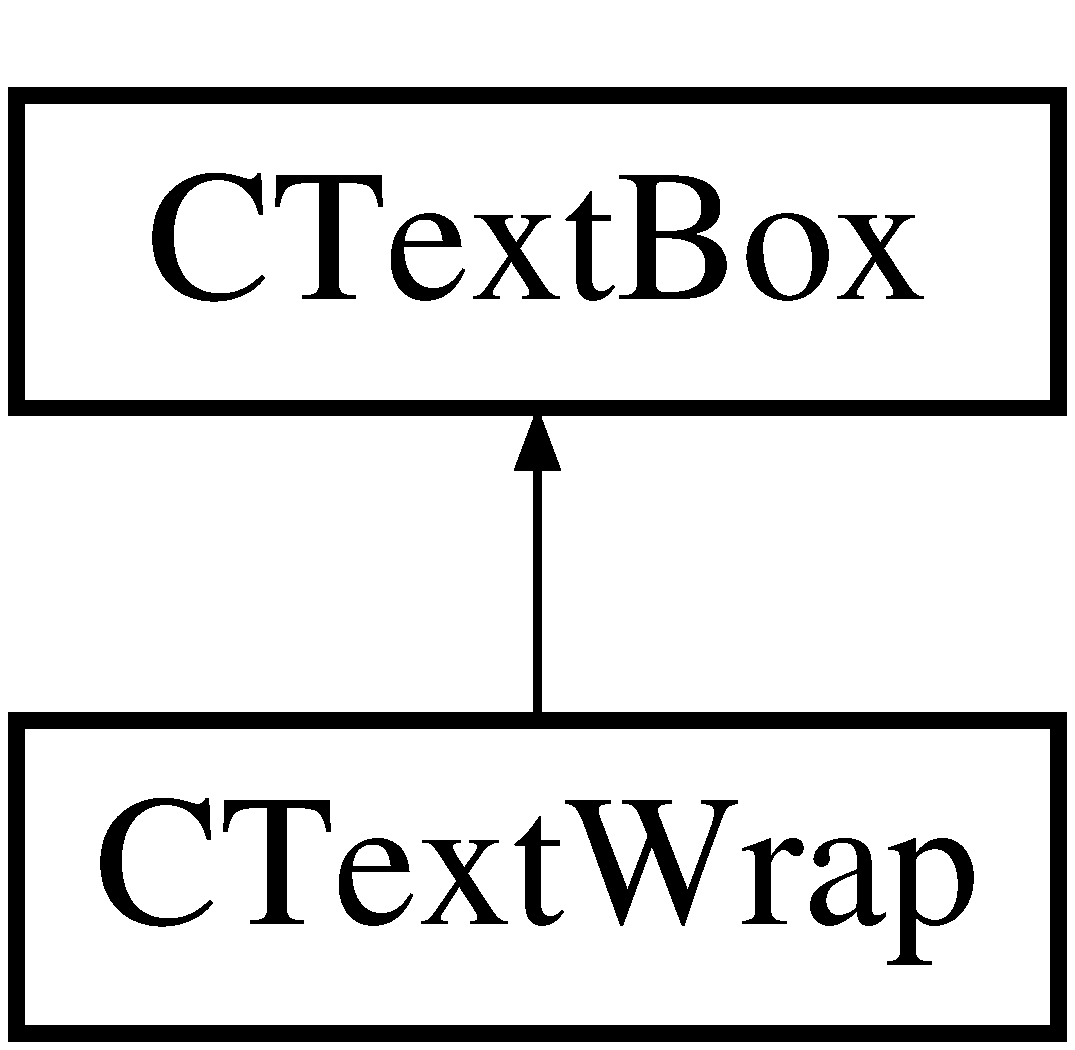
\includegraphics[height=2.000000cm]{class_c_text_wrap}
\end{center}
\end{figure}
\subsection*{Public Member Functions}
\begin{DoxyCompactItemize}
\item 
void {\bfseries Term} (\hyperlink{class_c_cmd_list}{C\+Cmd\+List} $\ast$\+\_\+cmdlist)\hypertarget{class_c_text_wrap_aa1fa97483e6a27ae37833d93de0775d8}{}\label{class_c_text_wrap_aa1fa97483e6a27ae37833d93de0775d8}

\item 
void {\bfseries Draw} (bool \+\_\+showingstop=false)\hypertarget{class_c_text_wrap_ac4347cc9888d7b72704be3d4d5da6c0a}{}\label{class_c_text_wrap_ac4347cc9888d7b72704be3d4d5da6c0a}

\end{DoxyCompactItemize}
\subsection*{Additional Inherited Members}


The documentation for this class was generated from the following files\+:\begin{DoxyCompactItemize}
\item 
Classes/Text\+Wrap.\+h\item 
Classes/Text\+Wrap.\+cpp\end{DoxyCompactItemize}

\hypertarget{class_c_trick_damage_effect}{}\section{C\+Trick\+Damage\+Effect Class Reference}
\label{class_c_trick_damage_effect}\index{C\+Trick\+Damage\+Effect@{C\+Trick\+Damage\+Effect}}
Inheritance diagram for C\+Trick\+Damage\+Effect\+:\begin{figure}[H]
\begin{center}
\leavevmode
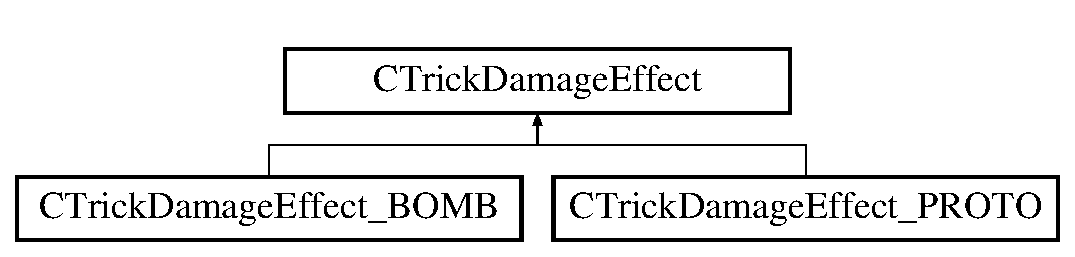
\includegraphics[height=2.000000cm]{class_c_trick_damage_effect}
\end{center}
\end{figure}
\subsection*{Public Member Functions}
\begin{DoxyCompactItemize}
\item 
{\bfseries C\+Trick\+Damage\+Effect} (std\+::string \+\_\+name)\hypertarget{class_c_trick_damage_effect_acec98051ffc3a877bd951361979e6512}{}\label{class_c_trick_damage_effect_acec98051ffc3a877bd951361979e6512}

\item 
virtual void {\bfseries Draw\+Damage\+Effect} (\hyperlink{class_c_battle}{C\+Battle} $\ast$\+\_\+battle, \hyperlink{class_c_b_img_bank}{C\+B\+Img\+Bank} $\ast$\+\_\+bimgbank, \hyperlink{class_c_rect}{C\+Rect} \+\_\+attackerR, \hyperlink{class_c_rect}{C\+Rect} \+\_\+targetR) const  =0\hypertarget{class_c_trick_damage_effect_ad13370446279773d91d842472dd9f8f9}{}\label{class_c_trick_damage_effect_ad13370446279773d91d842472dd9f8f9}

\item 
std\+::string {\bfseries Get\+Name} () const \hypertarget{class_c_trick_damage_effect_aabeea6bf435c8fc11645c1bb3761be1f}{}\label{class_c_trick_damage_effect_aabeea6bf435c8fc11645c1bb3761be1f}

\end{DoxyCompactItemize}
\subsection*{Protected Attributes}
\begin{DoxyCompactItemize}
\item 
std\+::string {\bfseries Name}\hypertarget{class_c_trick_damage_effect_a5e03077b434b9b00aeff2b0c64a4d065}{}\label{class_c_trick_damage_effect_a5e03077b434b9b00aeff2b0c64a4d065}

\end{DoxyCompactItemize}


The documentation for this class was generated from the following file\+:\begin{DoxyCompactItemize}
\item 
Classes/Trick\+Damage\+Effect.\+h\end{DoxyCompactItemize}

\hypertarget{class_c_trick_damage_effect___b_o_m_b}{}\section{C\+Trick\+Damage\+Effect\+\_\+\+B\+O\+MB Class Reference}
\label{class_c_trick_damage_effect___b_o_m_b}\index{C\+Trick\+Damage\+Effect\+\_\+\+B\+O\+MB@{C\+Trick\+Damage\+Effect\+\_\+\+B\+O\+MB}}
Inheritance diagram for C\+Trick\+Damage\+Effect\+\_\+\+B\+O\+MB\+:\begin{figure}[H]
\begin{center}
\leavevmode
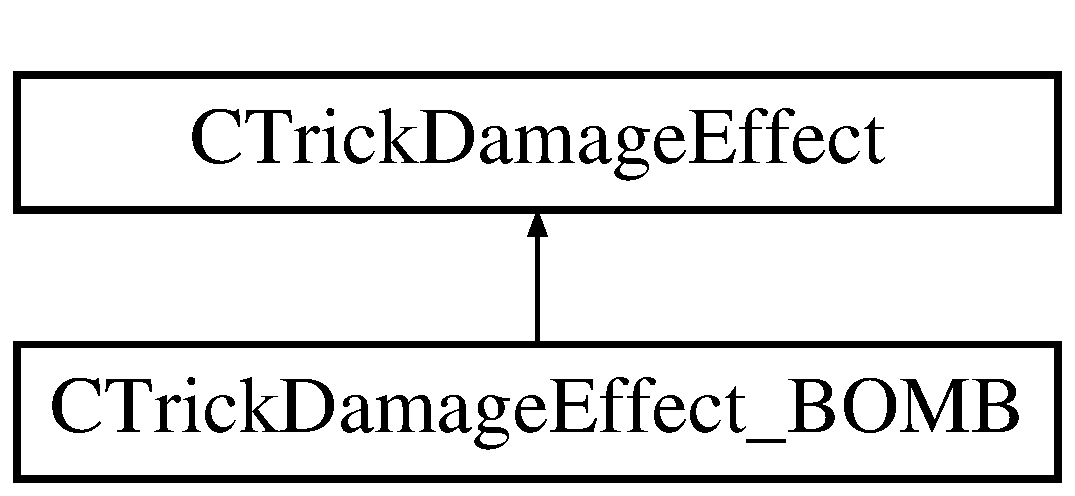
\includegraphics[height=2.000000cm]{class_c_trick_damage_effect___b_o_m_b}
\end{center}
\end{figure}
\subsection*{Public Member Functions}
\begin{DoxyCompactItemize}
\item 
{\bfseries C\+Trick\+Damage\+Effect\+\_\+\+B\+O\+MB} (std\+::string \+\_\+name, std\+::vector$<$ std\+::string $>$\+\_\+arg\+List)\hypertarget{class_c_trick_damage_effect___b_o_m_b_a66e2cc8b04b3f9dcbcdf3bd0ae4cc25d}{}\label{class_c_trick_damage_effect___b_o_m_b_a66e2cc8b04b3f9dcbcdf3bd0ae4cc25d}

\item 
void {\bfseries Draw\+Damage\+Effect} (\hyperlink{class_c_battle}{C\+Battle} $\ast$\+\_\+battle, \hyperlink{class_c_b_img_bank}{C\+B\+Img\+Bank} $\ast$\+\_\+bimgbank, \hyperlink{class_c_rect}{C\+Rect} \+\_\+attackerR, \hyperlink{class_c_rect}{C\+Rect} \+\_\+targetR) const \hypertarget{class_c_trick_damage_effect___b_o_m_b_a41bf6b8d8996188a5ee422482df85e39}{}\label{class_c_trick_damage_effect___b_o_m_b_a41bf6b8d8996188a5ee422482df85e39}

\end{DoxyCompactItemize}
\subsection*{Additional Inherited Members}


The documentation for this class was generated from the following files\+:\begin{DoxyCompactItemize}
\item 
Classes/Trick\+Damage\+Effect.\+h\item 
Classes/Trick\+Damage\+Effect.\+cpp\end{DoxyCompactItemize}

\hypertarget{class_c_trick_damage_effect___p_r_o_t_o}{}\section{C\+Trick\+Damage\+Effect\+\_\+\+P\+R\+O\+TO Class Reference}
\label{class_c_trick_damage_effect___p_r_o_t_o}\index{C\+Trick\+Damage\+Effect\+\_\+\+P\+R\+O\+TO@{C\+Trick\+Damage\+Effect\+\_\+\+P\+R\+O\+TO}}
Inheritance diagram for C\+Trick\+Damage\+Effect\+\_\+\+P\+R\+O\+TO\+:\begin{figure}[H]
\begin{center}
\leavevmode
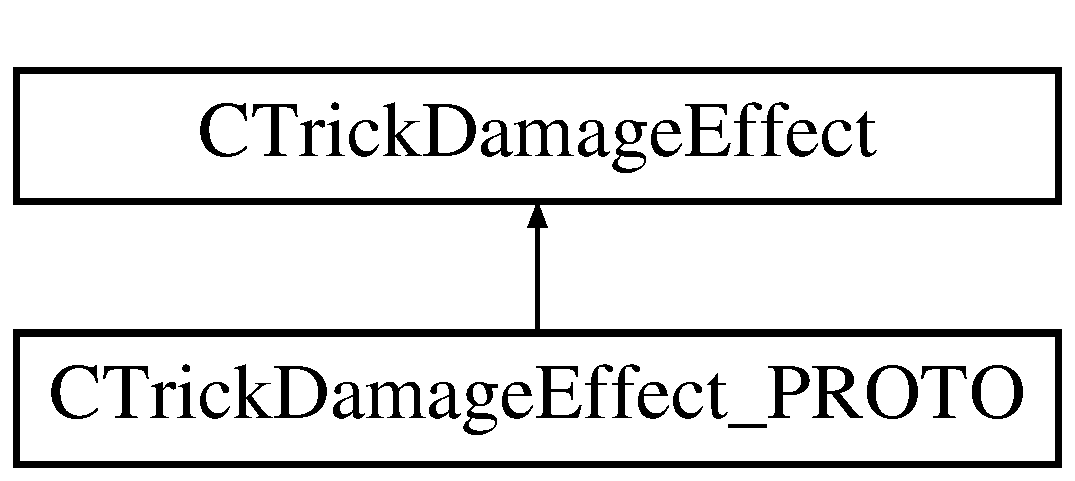
\includegraphics[height=2.000000cm]{class_c_trick_damage_effect___p_r_o_t_o}
\end{center}
\end{figure}
\subsection*{Public Member Functions}
\begin{DoxyCompactItemize}
\item 
{\bfseries C\+Trick\+Damage\+Effect\+\_\+\+P\+R\+O\+TO} (std\+::string \+\_\+name, std\+::vector$<$ std\+::string $>$\+\_\+arg\+List)\hypertarget{class_c_trick_damage_effect___p_r_o_t_o_a8ab1a6483da6ba6823f9c458c068dae2}{}\label{class_c_trick_damage_effect___p_r_o_t_o_a8ab1a6483da6ba6823f9c458c068dae2}

\item 
void {\bfseries Draw\+Damage\+Effect} (\hyperlink{class_c_battle}{C\+Battle} $\ast$\+\_\+battle, \hyperlink{class_c_b_img_bank}{C\+B\+Img\+Bank} $\ast$\+\_\+bimgbank, \hyperlink{class_c_rect}{C\+Rect} \+\_\+attackerR, \hyperlink{class_c_rect}{C\+Rect} \+\_\+targetR) const \hypertarget{class_c_trick_damage_effect___p_r_o_t_o_a658f84618db2d90386c0802672089137}{}\label{class_c_trick_damage_effect___p_r_o_t_o_a658f84618db2d90386c0802672089137}

\end{DoxyCompactItemize}
\subsection*{Additional Inherited Members}


The documentation for this class was generated from the following files\+:\begin{DoxyCompactItemize}
\item 
Classes/Trick\+Damage\+Effect.\+h\item 
Classes/Trick\+Damage\+Effect.\+cpp\end{DoxyCompactItemize}

\hypertarget{class_c_trick_manager}{}\section{C\+Trick\+Manager Class Reference}
\label{class_c_trick_manager}\index{C\+Trick\+Manager@{C\+Trick\+Manager}}
\subsection*{Public Member Functions}
\begin{DoxyCompactItemize}
\item 
void {\bfseries Add} (\hyperlink{structtrick__tag}{trick\+\_\+tag} \+\_\+trick, const char $\ast$\+\_\+key)\hypertarget{class_c_trick_manager_a4ff14d768273432dbb42c4107b9788f7}{}\label{class_c_trick_manager_a4ff14d768273432dbb42c4107b9788f7}

\item 
void {\bfseries Add} (char \+\_\+name\mbox{[}32\mbox{]}, int \+\_\+level, int \+\_\+cost, int \+\_\+time, target\+\_\+tag\+::type \+\_\+target\+Type, std\+::string \+\_\+damage\+Effect\+Name, std\+::vector$<$ \hyperlink{structside_effect__tag}{side\+Effect\+\_\+tag} $>$ side\+Effect\+List)\hypertarget{class_c_trick_manager_a977362fc3b7b6a5ac2d8cf790a516e9d}{}\label{class_c_trick_manager_a977362fc3b7b6a5ac2d8cf790a516e9d}

\item 
void {\bfseries Clear} ()\hypertarget{class_c_trick_manager_a3cdaa23673efbd07cd9192e1edbefb4c}{}\label{class_c_trick_manager_a3cdaa23673efbd07cd9192e1edbefb4c}

\item 
\hyperlink{structtrick__tag}{trick\+\_\+tag} const $\ast$ {\bfseries Get\+Trick} (const char \+\_\+name\mbox{[}32\mbox{]}, bool \+\_\+error\+Message=false)\hypertarget{class_c_trick_manager_a6df35ab36d8ccdf5915acfe58792cb88}{}\label{class_c_trick_manager_a6df35ab36d8ccdf5915acfe58792cb88}

\item 
void {\bfseries Create\+Damage\+Effect} (std\+::string \+\_\+type\+Name, std\+::string \+\_\+effect\+Name, std\+::vector$<$ std\+::string $>$\+\_\+arg\+List)\hypertarget{class_c_trick_manager_a1331fd57ddf7d938a1e3312686bf78e5}{}\label{class_c_trick_manager_a1331fd57ddf7d938a1e3312686bf78e5}

\item 
int {\bfseries Get\+Trick\+Damage\+Effect\+Index} (std\+::string \+\_\+name)\hypertarget{class_c_trick_manager_a855acdc647cb57daf01610de4827b6cf}{}\label{class_c_trick_manager_a855acdc647cb57daf01610de4827b6cf}

\item 
void {\bfseries Draw\+Effect} (int \+\_\+effect\+Index, \hyperlink{class_c_battle}{C\+Battle} $\ast$\+\_\+battle, \hyperlink{class_c_b_img_bank}{C\+B\+Img\+Bank} $\ast$\+\_\+bimgbank, \hyperlink{class_c_rect}{C\+Rect} \+\_\+attackerR, \hyperlink{class_c_rect}{C\+Rect} \+\_\+targetR)\hypertarget{class_c_trick_manager_ae1e882403baed30c569faa88886ad626}{}\label{class_c_trick_manager_ae1e882403baed30c569faa88886ad626}

\item 
void {\bfseries Debug\+Show\+Side\+Effect} (std\+::vector$<$ \hyperlink{structside_effect__tag}{side\+Effect\+\_\+tag} $>$ \+\_\+side\+Effect\+List)\hypertarget{class_c_trick_manager_a8c64cadcba83604210eb7a9c1b2d761d}{}\label{class_c_trick_manager_a8c64cadcba83604210eb7a9c1b2d761d}

\end{DoxyCompactItemize}
\subsection*{Static Public Member Functions}
\begin{DoxyCompactItemize}
\item 
static \hyperlink{class_c_trick_manager}{C\+Trick\+Manager} $\ast$ {\bfseries Get\+Instance} ()\hypertarget{class_c_trick_manager_a0de3b7589935108977cd708b68cc9196}{}\label{class_c_trick_manager_a0de3b7589935108977cd708b68cc9196}

\end{DoxyCompactItemize}


The documentation for this class was generated from the following files\+:\begin{DoxyCompactItemize}
\item 
Classes/Trick\+Manager.\+h\item 
Classes/Trick\+Manager.\+cpp\end{DoxyCompactItemize}

\hypertarget{class_c_vector}{}\section{C\+Vector Class Reference}
\label{class_c_vector}\index{C\+Vector@{C\+Vector}}


二次元座標用クラス////////////////////////////////////////  




{\ttfamily \#include $<$nunu\+Lib.\+h$>$}

\subsection*{Public Member Functions}
\begin{DoxyCompactItemize}
\item 
{\bfseries C\+Vector} (double \+\_\+x, double \+\_\+y)\hypertarget{class_c_vector_a451a6c62586656cfe33154149c105497}{}\label{class_c_vector_a451a6c62586656cfe33154149c105497}

\item 
void {\bfseries Set} (double \+\_\+x, double \+\_\+y)\hypertarget{class_c_vector_a2e2cc67a3107846821114920e756abab}{}\label{class_c_vector_a2e2cc67a3107846821114920e756abab}

\item 
void {\bfseries Set} (\hyperlink{class_c_vector}{C\+Vector} \+\_\+vec)\hypertarget{class_c_vector_a74b5df8d6cd2e914d416559c40c373f7}{}\label{class_c_vector_a74b5df8d6cd2e914d416559c40c373f7}

\item 
\hyperlink{class_c_vector}{C\+Vector} {\bfseries Add} (double \+\_\+x, double \+\_\+y)\hypertarget{class_c_vector_a932beef92cd5d375bd2542dff8a09c9d}{}\label{class_c_vector_a932beef92cd5d375bd2542dff8a09c9d}

\item 
\hyperlink{class_c_vector}{C\+Vector} {\bfseries Add} (\hyperlink{class_c_vector}{C\+Vector} \+\_\+vec)\hypertarget{class_c_vector_a05667e0f3cd5430b17477404532e37d4}{}\label{class_c_vector_a05667e0f3cd5430b17477404532e37d4}

\item 
\hyperlink{class_c_vector}{C\+Vector} {\bfseries operator+} (const \hyperlink{class_c_vector}{C\+Vector} \&obj)\hypertarget{class_c_vector_a6a08eefba0f23479f379c6501015988f}{}\label{class_c_vector_a6a08eefba0f23479f379c6501015988f}

\item 
\hyperlink{class_c_vector}{C\+Vector} {\bfseries operator+} (const double \+\_\+num)\hypertarget{class_c_vector_a9238a10280a584f3d6342d72f766d0fb}{}\label{class_c_vector_a9238a10280a584f3d6342d72f766d0fb}

\item 
\hyperlink{class_c_vector}{C\+Vector} \& {\bfseries operator+=} (const \hyperlink{class_c_vector}{C\+Vector} \&obj)\hypertarget{class_c_vector_a32a45e58ef2501f8609c8bddc31b42bb}{}\label{class_c_vector_a32a45e58ef2501f8609c8bddc31b42bb}

\item 
\hyperlink{class_c_vector}{C\+Vector} \& {\bfseries operator+=} (const double \+\_\+num)\hypertarget{class_c_vector_a6bb660e8b9e2cade677446a9881442bc}{}\label{class_c_vector_a6bb660e8b9e2cade677446a9881442bc}

\item 
\hyperlink{class_c_vector}{C\+Vector} {\bfseries operator-\/} (const \hyperlink{class_c_vector}{C\+Vector} \&obj)\hypertarget{class_c_vector_aeb8dd352b64ecbed41ebc098d36c9b33}{}\label{class_c_vector_aeb8dd352b64ecbed41ebc098d36c9b33}

\item 
\hyperlink{class_c_vector}{C\+Vector} {\bfseries operator-\/} (const double \+\_\+num)\hypertarget{class_c_vector_a79365afb400bbb6edfb68e9251ff7eb7}{}\label{class_c_vector_a79365afb400bbb6edfb68e9251ff7eb7}

\item 
\hyperlink{class_c_vector}{C\+Vector} \& {\bfseries operator-\/=} (const \hyperlink{class_c_vector}{C\+Vector} \&obj)\hypertarget{class_c_vector_abcd94112542fa9c8c2138545bb1fb869}{}\label{class_c_vector_abcd94112542fa9c8c2138545bb1fb869}

\item 
\hyperlink{class_c_vector}{C\+Vector} \& {\bfseries operator-\/=} (const double \+\_\+num)\hypertarget{class_c_vector_ac1fd0fa5b058c4abc0e4a708ce550627}{}\label{class_c_vector_ac1fd0fa5b058c4abc0e4a708ce550627}

\item 
\hyperlink{class_c_vector}{C\+Vector} {\bfseries operator$\ast$} (const \hyperlink{class_c_vector}{C\+Vector} \&obj)\hypertarget{class_c_vector_a29bd1257d790145597ba6a3f6f28b347}{}\label{class_c_vector_a29bd1257d790145597ba6a3f6f28b347}

\item 
\hyperlink{class_c_vector}{C\+Vector} {\bfseries operator$\ast$} (const double \+\_\+num)\hypertarget{class_c_vector_aff85de8cb73c04cb00cf02dfe4ca3605}{}\label{class_c_vector_aff85de8cb73c04cb00cf02dfe4ca3605}

\item 
\hyperlink{class_c_vector}{C\+Vector} \& {\bfseries operator$\ast$=} (const \hyperlink{class_c_vector}{C\+Vector} \&obj)\hypertarget{class_c_vector_acfe60a411a4d69a6b56b69dc83909a7d}{}\label{class_c_vector_acfe60a411a4d69a6b56b69dc83909a7d}

\item 
\hyperlink{class_c_vector}{C\+Vector} \& {\bfseries operator$\ast$=} (const double \+\_\+num)\hypertarget{class_c_vector_aecdf38377aa029969ebf53259bdd84c1}{}\label{class_c_vector_aecdf38377aa029969ebf53259bdd84c1}

\item 
double {\bfseries Get\+Length} ()\hypertarget{class_c_vector_a651ef9f5b622461f420996195b2a171d}{}\label{class_c_vector_a651ef9f5b622461f420996195b2a171d}

\end{DoxyCompactItemize}
\subsection*{Public Attributes}
\begin{DoxyCompactItemize}
\item 
double {\bfseries x}\hypertarget{class_c_vector_a937b4dfb43187450487dedb82c73c97c}{}\label{class_c_vector_a937b4dfb43187450487dedb82c73c97c}

\item 
double {\bfseries y}\hypertarget{class_c_vector_a4f7e8df6ec3e09a798ad785fd226e4a7}{}\label{class_c_vector_a4f7e8df6ec3e09a798ad785fd226e4a7}

\end{DoxyCompactItemize}


\subsection{Detailed Description}
二次元座標用クラス//////////////////////////////////////// 

The documentation for this class was generated from the following file\+:\begin{DoxyCompactItemize}
\item 
Classes/nunu\+Lib.\+h\end{DoxyCompactItemize}

\hypertarget{class_c_world_manager}{}\section{C\+World\+Manager Class Reference}
\label{class_c_world_manager}\index{C\+World\+Manager@{C\+World\+Manager}}
Inheritance diagram for C\+World\+Manager\+:\begin{figure}[H]
\begin{center}
\leavevmode
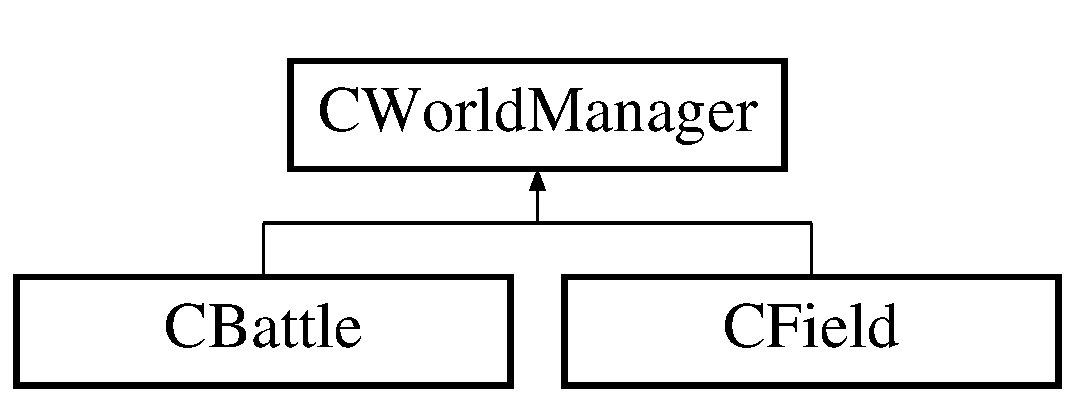
\includegraphics[height=2.000000cm]{class_c_world_manager}
\end{center}
\end{figure}
\subsection*{Public Member Functions}
\begin{DoxyCompactItemize}
\item 
virtual void {\bfseries Draw} (bool \+\_\+screenflip=false, bool \+\_\+textshowingstop=false, int dx=0, int dy=0, bool \+\_\+playeralsoshake=false)=0\hypertarget{class_c_world_manager_a3f437c19a8b23825c063edef74147008}{}\label{class_c_world_manager_a3f437c19a8b23825c063edef74147008}

\item 
void {\bfseries Fade\+Draw} (int \+\_\+time, int \+\_\+img, bool \+\_\+changeahead, bool \+\_\+color)\hypertarget{class_c_world_manager_adcd133e5c515b8e08af3afc8e4c63a81}{}\label{class_c_world_manager_adcd133e5c515b8e08af3afc8e4c63a81}

\item 
virtual void {\bfseries Change\+Text\+Mode} (bool \+\_\+box, const char $\ast$\+\_\+eventtext=N\+U\+LL)=0\hypertarget{class_c_world_manager_ac28db43e7e957665b586477a82120651}{}\label{class_c_world_manager_ac28db43e7e957665b586477a82120651}

\end{DoxyCompactItemize}
\subsection*{Protected Attributes}
\begin{DoxyCompactItemize}
\item 
int {\bfseries Img\+Back\+Ground}\hypertarget{class_c_world_manager_abde5850fe47cc2992bcd42a6e1a91b64}{}\label{class_c_world_manager_abde5850fe47cc2992bcd42a6e1a91b64}

\end{DoxyCompactItemize}


The documentation for this class was generated from the following files\+:\begin{DoxyCompactItemize}
\item 
Classes/World\+Manager.\+h\item 
Classes/World\+Manager.\+cpp\end{DoxyCompactItemize}

\hypertarget{structflag__tag}{}\section{flag\+\_\+tag Struct Reference}
\label{structflag__tag}\index{flag\+\_\+tag@{flag\+\_\+tag}}
\subsection*{Public Attributes}
\begin{DoxyCompactItemize}
\item 
char {\bfseries Key} \mbox{[}32\mbox{]}\hypertarget{structflag__tag_a1c25ae1024d23cc53467708833633e42}{}\label{structflag__tag_a1c25ae1024d23cc53467708833633e42}

\item 
int {\bfseries Num}\hypertarget{structflag__tag_a519bdb1ce1be06e65a18f9bc70da7f49}{}\label{structflag__tag_a519bdb1ce1be06e65a18f9bc70da7f49}

\end{DoxyCompactItemize}


The documentation for this struct was generated from the following file\+:\begin{DoxyCompactItemize}
\item 
Classes/Define.\+h\end{DoxyCompactItemize}

\hypertarget{class_hello_world}{}\section{Hello\+World Class Reference}
\label{class_hello_world}\index{Hello\+World@{Hello\+World}}
Inheritance diagram for Hello\+World\+:\begin{figure}[H]
\begin{center}
\leavevmode
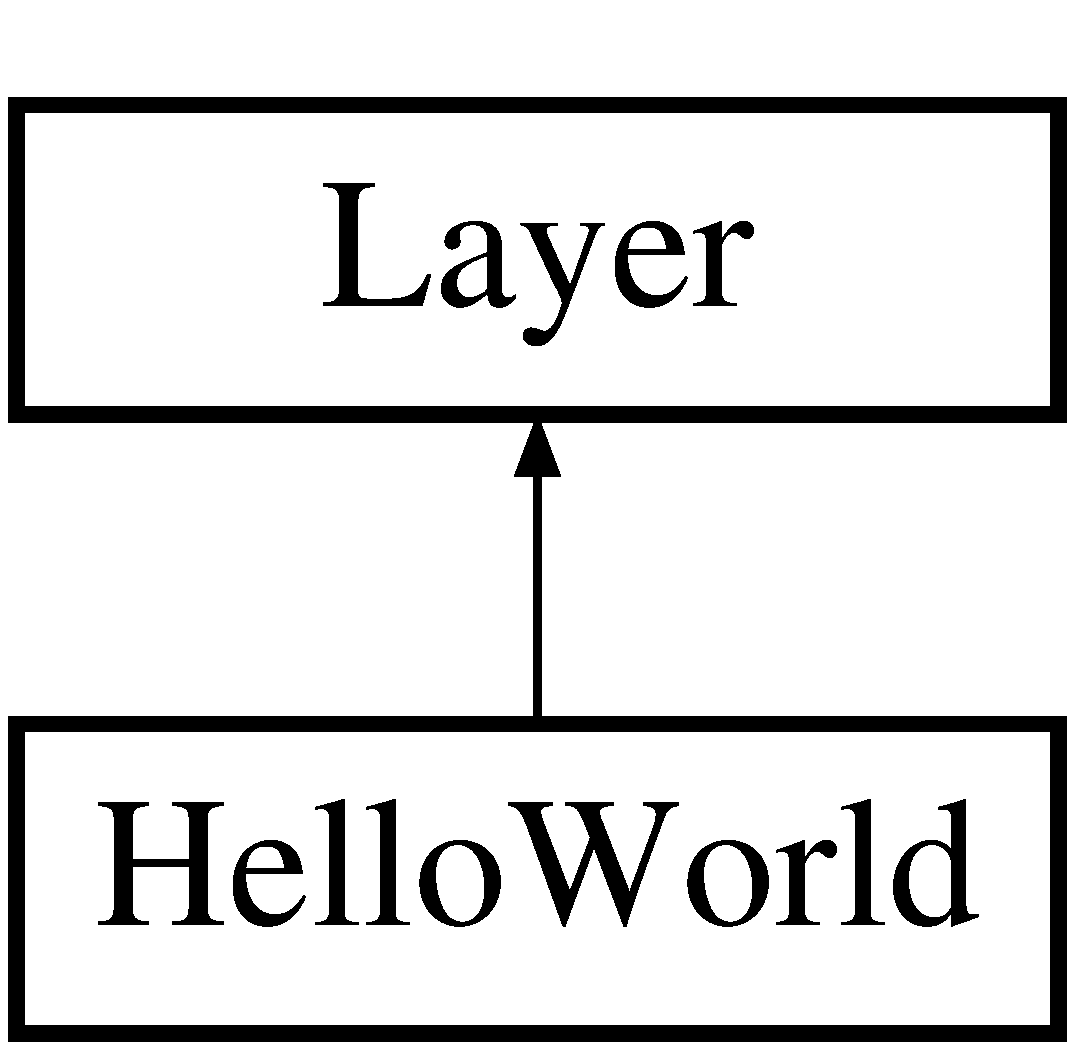
\includegraphics[height=2.000000cm]{class_hello_world}
\end{center}
\end{figure}
\subsection*{Public Member Functions}
\begin{DoxyCompactItemize}
\item 
virtual bool {\bfseries init} ()\hypertarget{class_hello_world_a65e2b1525051f3690e5a39ca56608a97}{}\label{class_hello_world_a65e2b1525051f3690e5a39ca56608a97}

\item 
void {\bfseries menu\+Close\+Callback} (cocos2d\+::\+Ref $\ast$p\+Sender)\hypertarget{class_hello_world_ac4ab2f5e922e659d4f137591c0f6a9b0}{}\label{class_hello_world_ac4ab2f5e922e659d4f137591c0f6a9b0}

\item 
{\bfseries C\+R\+E\+A\+T\+E\+\_\+\+F\+U\+NC} (\hyperlink{class_hello_world}{Hello\+World})\hypertarget{class_hello_world_a857ebfbc49f3a7f81772bee4991d186b}{}\label{class_hello_world_a857ebfbc49f3a7f81772bee4991d186b}

\end{DoxyCompactItemize}
\subsection*{Static Public Member Functions}
\begin{DoxyCompactItemize}
\item 
static cocos2d\+::\+Scene $\ast$ {\bfseries create\+Scene} ()\hypertarget{class_hello_world_a1b700f5f9de04271533d3fa099d7b014}{}\label{class_hello_world_a1b700f5f9de04271533d3fa099d7b014}

\end{DoxyCompactItemize}


The documentation for this class was generated from the following files\+:\begin{DoxyCompactItemize}
\item 
Classes/Hello\+World\+Scene.\+h\item 
Classes/Hello\+World\+Scene.\+cpp\end{DoxyCompactItemize}

\hypertarget{struct_c_enemy_species_manager_1_1encount__tag_1_1party__tag}{}\section{C\+Enemy\+Species\+Manager\+:\+:encount\+\_\+tag\+:\+:party\+\_\+tag Struct Reference}
\label{struct_c_enemy_species_manager_1_1encount__tag_1_1party__tag}\index{C\+Enemy\+Species\+Manager\+::encount\+\_\+tag\+::party\+\_\+tag@{C\+Enemy\+Species\+Manager\+::encount\+\_\+tag\+::party\+\_\+tag}}
\subsection*{Public Attributes}
\begin{DoxyCompactItemize}
\item 
int {\bfseries per}\hypertarget{struct_c_enemy_species_manager_1_1encount__tag_1_1party__tag_abd235dd819697b7932d093084228982e}{}\label{struct_c_enemy_species_manager_1_1encount__tag_1_1party__tag_abd235dd819697b7932d093084228982e}

\item 
std\+::vector$<$ \hyperlink{class_c_enemy_species}{C\+Enemy\+Species} $\ast$ $>$ {\bfseries party}\hypertarget{struct_c_enemy_species_manager_1_1encount__tag_1_1party__tag_a7b7fb8ccde65967a4627fc97e1e7a593}{}\label{struct_c_enemy_species_manager_1_1encount__tag_1_1party__tag_a7b7fb8ccde65967a4627fc97e1e7a593}

\end{DoxyCompactItemize}


The documentation for this struct was generated from the following file\+:\begin{DoxyCompactItemize}
\item 
Classes/Enemy\+Species\+Manager.\+h\end{DoxyCompactItemize}

\hypertarget{structplaydata__tag}{}\section{playdata\+\_\+tag Struct Reference}
\label{structplaydata__tag}\index{playdata\+\_\+tag@{playdata\+\_\+tag}}
\subsection*{Public Attributes}
\begin{DoxyCompactItemize}
\item 
bool {\bfseries Exist}\hypertarget{structplaydata__tag_a5a5fde508ceeaf7a5aa6589b565985c0}{}\label{structplaydata__tag_a5a5fde508ceeaf7a5aa6589b565985c0}

\item 
int {\bfseries Now\+Map}\hypertarget{structplaydata__tag_a5af9cd520612ed3e45810981ca2a5eb7}{}\label{structplaydata__tag_a5af9cd520612ed3e45810981ca2a5eb7}

\item 
unsigned int {\bfseries X}\hypertarget{structplaydata__tag_a3e96df391e27d23b8950916782d7bb0f}{}\label{structplaydata__tag_a3e96df391e27d23b8950916782d7bb0f}

\item 
unsigned int {\bfseries Y}\hypertarget{structplaydata__tag_aaecb1ccdf1d6fd8eabc476882fc8fc23}{}\label{structplaydata__tag_aaecb1ccdf1d6fd8eabc476882fc8fc23}

\item 
unsigned int {\bfseries OldX}\hypertarget{structplaydata__tag_a95c63de23c58a0f979e1348ddc6a3feb}{}\label{structplaydata__tag_a95c63de23c58a0f979e1348ddc6a3feb}

\item 
unsigned int {\bfseries OldY}\hypertarget{structplaydata__tag_afcce849212d7e645100856479276c907}{}\label{structplaydata__tag_afcce849212d7e645100856479276c907}

\item 
char {\bfseries Player\+Pic\+Key} \mbox{[}32\mbox{]}\hypertarget{structplaydata__tag_ae2f7dca12adefcf0736640651221aa4e}{}\label{structplaydata__tag_ae2f7dca12adefcf0736640651221aa4e}

\item 
enum direction\+\_\+tag {\bfseries Dir}\hypertarget{structplaydata__tag_a707b22684060dca47aeda1f4ad465bc6}{}\label{structplaydata__tag_a707b22684060dca47aeda1f4ad465bc6}

\item 
int {\bfseries Step}\hypertarget{structplaydata__tag_a6900f6671dde8a1f14e56753baaee52f}{}\label{structplaydata__tag_a6900f6671dde8a1f14e56753baaee52f}

\item 
int {\bfseries Dx}\hypertarget{structplaydata__tag_afbd0f88682d046acd1a896e064cc157b}{}\label{structplaydata__tag_afbd0f88682d046acd1a896e064cc157b}

\item 
int {\bfseries Dy}\hypertarget{structplaydata__tag_a0574ab388dad78bd9c40a2125717c6e1}{}\label{structplaydata__tag_a0574ab388dad78bd9c40a2125717c6e1}

\item 
bool {\bfseries Visible}\hypertarget{structplaydata__tag_a7172b1c4330eb858d646898116fc7d11}{}\label{structplaydata__tag_a7172b1c4330eb858d646898116fc7d11}

\item 
\hyperlink{class_c_flag_set}{C\+Flag\+Set} {\bfseries Flag\+Set}\hypertarget{structplaydata__tag_aec35284b6a85e346900aa7bf6781b4ac}{}\label{structplaydata__tag_aec35284b6a85e346900aa7bf6781b4ac}

\item 
std\+::vector$<$ \hyperlink{class_c_eve_obj}{C\+Eve\+Obj} $>$ {\bfseries Eve\+Obj}\hypertarget{structplaydata__tag_ab52fc1c0aa50892765d9fc04b690f0b7}{}\label{structplaydata__tag_ab52fc1c0aa50892765d9fc04b690f0b7}

\item 
char {\bfseries Data\+Name} \mbox{[}32\mbox{]}\hypertarget{structplaydata__tag_ae85951906fa3142ae9775b43e1ab1cb1}{}\label{structplaydata__tag_ae85951906fa3142ae9775b43e1ab1cb1}

\end{DoxyCompactItemize}


The documentation for this struct was generated from the following file\+:\begin{DoxyCompactItemize}
\item 
Classes/Define.\+h\end{DoxyCompactItemize}

\hypertarget{struct_c_text_box_1_1ruby__tag}{}\section{C\+Text\+Box\+:\+:ruby\+\_\+tag Struct Reference}
\label{struct_c_text_box_1_1ruby__tag}\index{C\+Text\+Box\+::ruby\+\_\+tag@{C\+Text\+Box\+::ruby\+\_\+tag}}
\subsection*{Public Attributes}
\begin{DoxyCompactItemize}
\item 
char {\bfseries Word} \mbox{[}32\mbox{]}\hypertarget{struct_c_text_box_1_1ruby__tag_a29e36b52fd55c8e1807c9d2b9a938772}{}\label{struct_c_text_box_1_1ruby__tag_a29e36b52fd55c8e1807c9d2b9a938772}

\item 
char {\bfseries Ruby} \mbox{[}32\mbox{]}\hypertarget{struct_c_text_box_1_1ruby__tag_a9ba237f4d6dccde17904b2310194364c}{}\label{struct_c_text_box_1_1ruby__tag_a9ba237f4d6dccde17904b2310194364c}

\item 
char {\bfseries ch\+Num} \mbox{[}3\mbox{]}\hypertarget{struct_c_text_box_1_1ruby__tag_aeeb75c45699d70f39ffd7b43531f84f3}{}\label{struct_c_text_box_1_1ruby__tag_aeeb75c45699d70f39ffd7b43531f84f3}

\end{DoxyCompactItemize}


The documentation for this struct was generated from the following file\+:\begin{DoxyCompactItemize}
\item 
Classes/Text\+Box.\+h\end{DoxyCompactItemize}

\hypertarget{structside_effect__tag}{}\section{side\+Effect\+\_\+tag Struct Reference}
\label{structside_effect__tag}\index{side\+Effect\+\_\+tag@{side\+Effect\+\_\+tag}}
\subsection*{Public Member Functions}
\begin{DoxyCompactItemize}
\item 
{\bfseries E\+N\+UM} (type\+\_\+tag, A\+TK, D\+EF, S\+PD, H\+E\+AL, M\+P\+H\+E\+AL, A\+T\+T\+E\+N\+T\+I\+ON, S\+E\+T\+\_\+\+T\+I\+M\+E\+G\+A\+U\+GE, H\+E\+A\+L\+\_\+\+A\+F\+T\+E\+R\+\_\+\+A\+T\+T\+A\+CK, H\+E\+A\+L\+\_\+\+A\+F\+T\+E\+R\+\_\+\+S\+E\+L\+E\+C\+T\+C\+O\+M\+M\+A\+ND)\hypertarget{structside_effect__tag_ab82e228f131bb664c7478d25e11c8b31}{}\label{structside_effect__tag_ab82e228f131bb664c7478d25e11c8b31}

\end{DoxyCompactItemize}
\subsection*{Public Attributes}
\begin{DoxyCompactItemize}
\item 
type\+\_\+tag\+::type {\bfseries Effect\+Type}\hypertarget{structside_effect__tag_af4647ccd1d4b3556cff1a6ffb886a15d}{}\label{structside_effect__tag_af4647ccd1d4b3556cff1a6ffb886a15d}

\item 
target\+\_\+tag\+::type {\bfseries Effect\+Target}\hypertarget{structside_effect__tag_a7b2b8eaa0df7c695295bcf235a8b7299}{}\label{structside_effect__tag_a7b2b8eaa0df7c695295bcf235a8b7299}

\item 
int {\bfseries Power}\hypertarget{structside_effect__tag_a6b30d47d6310a64e26017b1ecba11a39}{}\label{structside_effect__tag_a6b30d47d6310a64e26017b1ecba11a39}

\item 
int {\bfseries Incidence}\hypertarget{structside_effect__tag_a7f184e69f6f5638a8fdca52ddf7335de}{}\label{structside_effect__tag_a7f184e69f6f5638a8fdca52ddf7335de}

\item 
int {\bfseries Time}\hypertarget{structside_effect__tag_ad99ad9b24a1bac25882bcf7bf6fa648a}{}\label{structside_effect__tag_ad99ad9b24a1bac25882bcf7bf6fa648a}

\end{DoxyCompactItemize}


The documentation for this struct was generated from the following file\+:\begin{DoxyCompactItemize}
\item 
Classes/Define.\+h\end{DoxyCompactItemize}

\hypertarget{structstatus_changer__tag}{}\section{status\+Changer\+\_\+tag Struct Reference}
\label{structstatus_changer__tag}\index{status\+Changer\+\_\+tag@{status\+Changer\+\_\+tag}}
\subsection*{Public Attributes}
\begin{DoxyCompactItemize}
\item 
int {\bfseries Img}\hypertarget{structstatus_changer__tag_a6082189f596075c2c27c72a22f35dc12}{}\label{structstatus_changer__tag_a6082189f596075c2c27c72a22f35dc12}

\item 
double {\bfseries Time}\hypertarget{structstatus_changer__tag_a423795cf8f6e0298eba6badf5ab0a7b8}{}\label{structstatus_changer__tag_a423795cf8f6e0298eba6badf5ab0a7b8}

\item 
int {\bfseries Status\+Kind}\hypertarget{structstatus_changer__tag_a68bed5d94327f1f3a7638c80c7b76448}{}\label{structstatus_changer__tag_a68bed5d94327f1f3a7638c80c7b76448}

\item 
int {\bfseries Power}\hypertarget{structstatus_changer__tag_abd9ff21ed0f7a75fc9eafa149352447e}{}\label{structstatus_changer__tag_abd9ff21ed0f7a75fc9eafa149352447e}

\end{DoxyCompactItemize}


The documentation for this struct was generated from the following file\+:\begin{DoxyCompactItemize}
\item 
Classes/Define.\+h\end{DoxyCompactItemize}

\hypertarget{structtrick__tag}{}\section{trick\+\_\+tag Struct Reference}
\label{structtrick__tag}\index{trick\+\_\+tag@{trick\+\_\+tag}}
\subsection*{Public Attributes}
\begin{DoxyCompactItemize}
\item 
char {\bfseries Name} \mbox{[}32\mbox{]}\hypertarget{structtrick__tag_a19f10c215adf43633d12dd93e5a32b6e}{}\label{structtrick__tag_a19f10c215adf43633d12dd93e5a32b6e}

\item 
int {\bfseries Power}\hypertarget{structtrick__tag_a0fba9770964892006f897cd5c51f42b3}{}\label{structtrick__tag_a0fba9770964892006f897cd5c51f42b3}

\item 
int {\bfseries Cost}\hypertarget{structtrick__tag_a32e41cc02cb205223cd9b9f5cc0ee308}{}\label{structtrick__tag_a32e41cc02cb205223cd9b9f5cc0ee308}

\item 
int {\bfseries Time}\hypertarget{structtrick__tag_a05502ec2cc3492a6fbfd95f4fe1a4a63}{}\label{structtrick__tag_a05502ec2cc3492a6fbfd95f4fe1a4a63}

\item 
std\+::vector$<$ \hyperlink{structside_effect__tag}{side\+Effect\+\_\+tag} $>$ {\bfseries Side\+Effect}\hypertarget{structtrick__tag_a51a55706c976b33a7d1dcea66c31545f}{}\label{structtrick__tag_a51a55706c976b33a7d1dcea66c31545f}

\item 
int {\bfseries Damage\+Effect\+Index}\hypertarget{structtrick__tag_a7f90a4a3789d9368464a1a3628256666}{}\label{structtrick__tag_a7f90a4a3789d9368464a1a3628256666}

\item 
target\+\_\+tag\+::type {\bfseries Target}\hypertarget{structtrick__tag_aed4f67e34e35d771fde58c1448d4c39f}{}\label{structtrick__tag_aed4f67e34e35d771fde58c1448d4c39f}

\end{DoxyCompactItemize}


The documentation for this struct was generated from the following file\+:\begin{DoxyCompactItemize}
\item 
Classes/Define.\+h\end{DoxyCompactItemize}

%--- End generated contents ---

% Index
\backmatter
\newpage
\phantomsection
\clearemptydoublepage
\addcontentsline{toc}{chapter}{Index}
\printindex

\end{document}
